\documentclass[10pt]{extarticle}
\usepackage[letterpaper, bottom=1.4in]{geometry}
\usepackage{import}

\usepackage{enumerate}
\usepackage[table]{xcolor}
\usepackage{graphics}
\usepackage{graphicx}
\usepackage{mathrsfs}
\usepackage{multirow}
\usepackage{hhline}
\usepackage{pbox}
\usepackage{hyperref}
\usepackage{fancyhdr}
\usepackage{amsmath,amssymb,amsthm,esint}
\usepackage{longtable}
\usepackage{tikz}
\usepackage{float}
\usepackage{pgfplots}
\usepackage{caption}
\usepackage{subcaption}
\usepackage{empheq}
\usepackage{indentfirst}
\usepackage{algorithm}
\usepackage{algpseudocode}

\usepackage[many]{tcolorbox}
\usepackage[T1]{fontenc}
\usepackage[utf8]{inputenc}
\usepackage{lmodern}
\usepackage[english]{babel}
\newcommand{\wto}{\rightharpoonup}

\usepackage{makeidx}

\newtheorem{theorem}{Theorem}[section]
\newtheorem{acknowledgement}[theorem]{Acknowledgement}
%\newtheorem{algorithm}[theorem]{Algorithm}
\newtheorem{axiom}[theorem]{Axiom}
\newtheorem{case}[theorem]{Case}
\newtheorem{claim}[theorem]{Claim}
\newtheorem{conclusion}[theorem]{Conclusion}
\newtheorem{condition}[theorem]{Condition}
\newtheorem{conjecture}[theorem]{Conjecture}
\newtheorem{corollary}[theorem]{Corollary}
\newtheorem{criterion}[theorem]{Criterion}
\newtheorem{conditions}[theorem]{Conditions}
\newtheorem{definition}[theorem]{Definition}
\newtheorem{example}[theorem]{Example}
\newtheorem{exercise}{Exercise}
\newtheorem{lemma}[theorem]{Lemma}
\DeclareMathOperator*{\argmax}{arg\,max}
\DeclareMathOperator*{\argmin}{arg\,min}
\DeclarePairedDelimiter{\ceil}{\lceil}{\rceil}
\DeclarePairedDelimiter\floor{\lfloor}{\rfloor}


\newtheorem{proposition}[theorem]{Proposition}
%\newenvironment{proof}[1][Proof]{\noindent\textbf{#1.} }{\ \rule{0.5em}{0.5em}}
\newcommand{\e}{\varepsilon}
\newcommand{\relu}{\text{ReLU}}
\newcommand{\norm}[1]{\left\vert #1 \right\vert}
\newcommand{\Norm}[1]{\left\Vert #1 \right\Vert}
%\DeclareMathOperator*{\argmax}{arg\,max}
%\DeclareMathOperator*{\argmin}{arg\,min}
%\DeclarePairedDelimiter{\ceil}{\lceil}{\rceil}
%\DeclarePairedDelimiter\floor{\lfloor}{\rfloor}
\usepackage{todonotes}
\usepackage{amsmath}

%\usepackage{mathabx}


%%%%%%%%%%%%%%%% TIKZ stuff %%%%%%%%%%%%%%%%
    \pgfplotsset{compat=newest}
    \usetikzlibrary{shapes,arrows,matrix,positioning,intersections}
    \usetikzlibrary{calc}
%    \usetikzlibrary{decorations.pathreplacing}
    \usetikzlibrary{decorations} %fancier tikz abilities
    \pgfdeclarelayer{bg}
    \pgfsetlayers{bg,main}
		% Define block styles
    \tikzstyle{decision} = [diamond, draw, fill=blue!20, 
        text width=3cm, text badly centered, node distance=3cm, inner sep=0pt]
    \tikzstyle{block} = [rectangle, draw, fill=blue!20, 
        text width=3cm, text centered, rounded corners, minimum height=2em]
    \tikzstyle{line} = [draw, -latex']
    \tikzstyle{cloud} = [draw, ellipse,fill=red!20, node distance=3cm,
        minimum height=2em]

\usetikzlibrary{decorations.text,arrows.meta}
\usetikzlibrary{decorations.pathmorphing}
\usetikzlibrary{decorations.markings} %hopefully give arrows

\tikzset{
  % style to apply some styles to each segment of a path
  on each segment/.style={
    decorate,
    decoration={
      show path construction,
      moveto code={},
      lineto code={
        \path [#1]
        (\tikzinputsegmentfirst) -- (\tikzinputsegmentlast);
      },
      curveto code={
        \path [#1] (\tikzinputsegmentfirst)
        .. controls
        (\tikzinputsegmentsupporta) and (\tikzinputsegmentsupportb)
        ..
        (\tikzinputsegmentlast);
      },
      closepath code={
        \path [#1]
        (\tikzinputsegmentfirst) -- (\tikzinputsegmentlast);
      },
    },
  },
  % style to add an arrow in the middle of a path
  mid arrow/.style={postaction={decorate,decoration={
        markings,
        mark=at position .5 with {\arrow[#1]{stealth}}
      }}},
}

%%%%%%%%%%%%%%%% Table of Contents Stuff %%%%%%%%%%%%%%%%
\setcounter{secnumdepth}{3} % if set to -1 only chapter and sections will be numbered
\setcounter{tocdepth}{1}

%%%%%%%%%%%%%%%% Hyper Ref Stuff %%%%%%%%%%%%%%%%
		% set up reference style
\hypersetup{
    linktoc=all,		% build toc with internal links
    unicode=false,         	% non-Latin chars in Acrobat bookmarks
    pdftoolbar=true,       	% show Acrobats toolbar?
    pdfmenubar=true,       	% show Acrobats menu?
    pdffitwindow=false,    	% window fit to page when opened
    pdfstartview={FitH},   	% fits width of page to the window
    pdftitle={My title},   	% title
    pdfauthor={Author},    	% author
    pdfsubject={Subject},  	% subject of the document
    pdfcreator={Creator},  	% creator of the document
    pdfproducer={Producer},	% producer of the document
    pdfkeywords={keyword1} {key2} {key3}, % list of keywords
    pdfnewwindow=true,      	% links in new window
    colorlinks=true,       	% false: boxed links; true: colore links
    linkcolor=blue,          	% color of internal links (change box
				% color with linkbordercolor)
    citecolor=green,        	% color of links to bibliography
    filecolor=magenta,      	% color of file links
    urlcolor=cyan           	% color of external links
}

%%%%%%%%%%%%%%%% My Commands/Shorthand %%%%%%%%%%%%%%%%
% \newcommand{\qed}{\hfill\ensuremath{\Box}}

% \newcommand{\qedb}{\hfill \blacksquare}
% \newcommand{\LIM}{\text{LIM}}
% \newcommand{\wrt}{w.r.t}
% \newcommand{\rml}{\multicolumn{1}{c}{}}
% \newcommand{\tbf}[1]{\textbf{#1}}
% \newcommand{\ib}[1]{\item \textbf{#1}}
% \newcommand{\B}{\mathcal{B}}
% \newcommand{\R}{\mathbb{R}}

% \newcommand{\K}{\mathbb{K}}
% \newcommand{\F}{\mathbb{F}}
% \newcommand{\re}{\text{Re}}
% %\newcommand{\Z}{\mathbb{Z}}
% \newcommand{\TT}{\mathbb{T}}
% \newcommand{\T}{\mathcal{T}}
% %\newcommand{\S}{\mathcal{S}}
% \newcommand{\N}{\mathbb{N}}
% \newcommand{\M}{\mathcal{M}}
% \newcommand{\MO}{\mathcal{O}}
% \newcommand{\prob}{\text{Prob}}
% \newcommand{\var}{\text{Var}}
% \newcommand{\Q}{\mathbb{Q}}
% \newcommand{\C}{\mathbb{C}}
% \newcommand{\E}{\mathcal{E}}
% \newcommand{\fl}{\text{fl}}
% \newcommand{\sign}{\text{sign}}
\usepackage{bbm}
\newlength{\arrow}
\settowidth{\arrow}{\scriptsize argmax}
\newcommand*{\myrightarrow}[1]{\xrightarrow{\mathmakebox[\arrow]{#1}}}


% \newcommand*\circled[1]{\tikz[baseline=(char.base)]{
%             \node[shape=circle,draw,inner sep=2pt] (char) {#1};}}

% \newcommand{\nifty}{\textbf{NIFTY}}




\tcbset{breakable,
skin=bicolor,
colback=black!15!white,
colbacklower=white,
colframe=black!25!white,
coltitle=black,
fonttitle=\bfseries,
boxrule=1pt,
boxsep=3.0pt,
left=0.0pt,
right=0.0pt,
top=0.0pt,
bottom=0.0pt,
middle = 1.0pt,
arc = 0.0pt,
outer arc = 0.0pt,
frame style={top color=white,
bottom color=white,draw=black},
interior style={left color=black!0!white,right color=black!0!white},
segmentation style={right color=white,left color=white}
}

\DeclareMathOperator{\Tr}{Tr}


\author{Brian Bell : University of Arizona}
\date{\today}
\title{Neighborhoods of Adversarial Examples}

%%%%%%%%%%%%%%%% Title Stuff %%%%%%%%%%%%%%%%

% \IfFileExists{/dev/null}{\import{"\string~/Dropbox/UOFA/"}{headder}}{\import{"\string~/Google Drive/dropbox/Dropbox/UOFA/"}{headder}}




\makeindex
\usepackage[totoc]{idxlayout}%\makenoidxglossaries
%\makeglossaries
%\renewcommand{\baselinestretch}{1.5}
\setlength\parindent{24pt}
\usepackage{setspace}
\doublespacing

%%%%%%%%%%%%%%%% Color commands %%%%%%%%%%%%%%%%
\newcommand{\red}[1]{\textcolor{red}{#1}}
\newcommand{\blue}[1]{\textcolor{blue}{#1}}
\newcommand{\green}[1]{\textcolor{green}{#1}}

%%%%%%%%%%%%%%%% My Commands/Shorthand %%%%%%%%%%%%%%%%
%\newcommand{\qed}{\hfill\ensuremath{\Box}}
\newcommand{\qedb}{\hfill \blacksquare}
\newcommand{\wrt}{w.r.t}
\newcommand{\rml}{\multicolumn{1}{c}{}}
\newcommand{\tbf}[1]{\textbf{#1}}
\newcommand{\ib}[1]{\item \textbf{#1}}
\newcommand{\B}{\mathcal{B}}
\newcommand{\R}{\mathbb{R}}
\newcommand{\re}{\text{Re}}
%\newcommand{\Z}{\mathbb{Z}}
\newcommand{\TT}{\mathbb{T}}
\newcommand{\T}{\mathcal{T}}
%\newcommand{\S}{\mathcal{S}}
\newcommand{\N}{\mathbb{N}}
\newcommand{\X}{\mathcal{X}}
\newcommand{\M}{\mathcal{M}}
\newcommand{\MO}{\mathcal{O}}
\newcommand{\prob}{\text{Prob}}
\newcommand{\var}{\text{Var}}
\newcommand{\Q}{\mathbb{Q}}
\newcommand{\C}{\mathbb{C}}
\newcommand{\CC}{\mathcal{C}}
\newcommand{\fl}{\text{fl}}
\newcommand{\sign}{\text{sign}}

\newcommand{\ip}[1]{\left\langle #1 \right\rangle}
\def\tesst{https://chrome.google.com/webstore/detail/slack-bot-filter/blephhkggdennbfmdcjmlfimedknghfc}
\def\lvector#1{\underline{#1}}
\def\lmatrix#1{\underline{\underline{#1}}}
\def\ltensor#1{\underline{\underline{\underline{#1}}}}
\DeclareMathOperator\vol{\text{vol}}

\newcommand{\vectorproj}[2][]{\textit{proj}_{\vect{#1}}\vect{#2}}
\newcommand{\vect}{\mathbf}


\newcommand*\circled[1]{\tikz[baseline=(char.base)]{
            \node[shape=circle,draw,inner sep=2pt] (char) {#1};}}
\newcommand{\nifty}{\textbf{NIFTY}}



% Define block styles
\tikzstyle{decision} = [diamond, draw, fill=blue!20,
    text width=3cm, text badly centered, node distance=3cm, inner sep=0pt]
\tikzstyle{block} = [rectangle, draw, fill=blue!20,
    text width=3cm, text centered, rounded corners, minimum height=2em]
\tikzstyle{line} = [draw, -latex']
\tikzstyle{cloud} = [draw, ellipse,fill=red!20, node distance=3cm,
    minimum height=2em]

\newcommand\setrow[5]{
  \setcounter{col}{1}
  \foreach \n in {#1, #2, #3, #4, #5}{%, #6, #7, #8, #9} {
    \edef\x{\value{col} +.5}
    \edef\y{.5 + \value{row}}
    \node[anchor=center] at (\x, \y) {\n};
    \stepcounter{col}
  }
  \stepcounter{row}
}
\usepackage{mathpazo}
\newcounter{row}
\newcounter{col}

% \usepackage{enumerate}
% \newcommand{\e}{\varepsilon}
% \newcommand{\R}{\mathbb{R}}
 %\newcommand{\T}{\mathcal{T}}
% \newcommand{\N}{\mathbb{N}}
% \newcommand{\prob}{\text{Prob}}
% \newcommand{\Q}{\mathbb{Q}}
% \newcommand{\C}{\mathbb{C}}
% \newcounter{test}
 \def\layersep{2.0cm}


% %\documentclass{beamer}

% \mode<presentation>
% {
%   \usetheme{Boadilla}
%   % possiblities Singapore, Malmoe, Dresden
%   \setbeamercovered{transparent}
% }


% %\setbeamertemplate{navigation symbols}{}
% % removes the navigation symbols

% %color setting more or less matching U of A colors
% \setbeamercolor*{palette secondary}{use=structure,fg=white,bg=structure.fg!55!black}
% \setbeamercolor*{palette tertiary}{use=structure,fg=white,bg=red!50!black}

% \usepackage[english]{babel}
% \usepackage[latin1]{inputenc}
% \usepackage{times}
% \usepackage[T1]{fontenc}
% \usepackage{graphicx}
% \usepackage{amsfonts}
% \usepackage{transparent}
% \usepackage{tikz}
% \usetikzlibrary{arrows,positioning,backgrounds,fit}

%%%%%%%%%%%%%%%%%%%%%%%%%%%%%%%%%%%%%%%%%%%%%%%%%%%%%%%%%%%%%%%%
\usepackage[utf8]{inputenc} % allow utf-8 input
\usepackage[T1]{fontenc}    % use 8-bit T1 fonts
\usepackage{hyperref}       % hyperlinks
\usepackage{calc}
\usepackage{url}            % simple URL typesetting
\usepackage{booktabs}       % professional-quality tables
\usepackage{amsfonts}       % blackboard math symbols
\usepackage{nicefrac}       % compact symbols for 1/2, etc.
\usepackage{microtype}      % microtypography
\usepackage{xcolor}         % colors
\usepackage{subcaption}
\newcommand{\RR}{I\!\!R} %real numbers
\newcommand{\Nat}{I\!\!N} %natural numbers
\usepackage{textcase}
\usepackage{thmtools,thm-restate}
\usepackage{subcaption}

\newlength{\depthofsumsign}
\setlength{\depthofsumsign}{\depthof{$\sum$}}
\newlength{\totalheightofsumsign}
\newlength{\heightanddepthofargument}

\newcommand{\nsum}[1][1.4]{% only for \displaystyle
    \mathop{%
        \raisebox
            {-#1\depthofsumsign+1\depthofsumsign}
            {\scalebox
                {#1}
                {$\displaystyle\sum$}%
            }
    }
}
\newcommand{\resum}[1]{%
    \def\s{#1}
    \mathop{
        \mathpalette\resumaux{#1}
    }
}

\newcommand{\resumaux}[2]{% internally
    \sbox0{$#1#2$}
    \sbox1{$#1\sum$}
    \setlength{\heightanddepthofargument}{\wd0+\dp0}
    \setlength{\totalheightofsumsign}{\wd1+\dp1}
    \def\quot{\DivideLengths{\heightanddepthofargument}{\totalheightofsumsign}}
    \nsum[\quot]%
}

% http://tex.stackexchange.com/a/6424/16595
\makeatletter
\newcommand*{\DivideLengths}[2]{%
  \strip@pt\dimexpr\number\numexpr\number\dimexpr#1\relax*65536/\number\dimexpr#2\relax\relax sp\relax
}
\makeatother


\usepackage{bbm}
\usepackage{algorithm}
\usepackage{algpseudocode}
\usepackage{booktabs}
\usepackage{pgfplots}
\usepackage{tikz-3dplot}
\usepackage{dsfont}

\tdplotsetmaincoords{60}{115}
\pgfplotsset{compat=newest}

%\newtheorem{theorem}{Theorem}[section]

%\newenvironment{proof}[1][Proof]{\noindent\textbf{#1.} }{\ \rule{0.5em}{0.5em}}
%\DeclareMathOperator*{\argmax}{arg\,max}
%\DeclareMathOperator*{\argmin}{arg\,min}
%\DeclarePairedDelimiter{\ceil}{\lceil}{\rceil}
%\DeclarePairedDelimiter\floor{\lfloor}{\rfloor}
\usepackage{todonotes}
\usepackage{amsmath}
\usepackage{mathtools}
%%%%%%%%%%%%%%%%%%%%%%%%%%%%%%%%%%%%%%%%%%%%%%%%%%%%%%%%%%%%%%%%

\begin{document}
\titlepage
\maketitle
\tableofcontents


\section{Introduction}

Artificial Neural Networks and other optimization-based general
function approximation models are the core of modern
machine learning \cite{prakash2018}. These models have dominated competitions in image processing, optical character recognition, object detection, video classification, natural language processing, and many other fields \cite{SCHMIDHUBER201585}. All such modern models are
trained via gradient-based optimization, e.g. Stochastic Gradient Descent (SGD) with
gradients computed via back propagation. \cite{goodfellow2013multidigit}. Although the performance of these models is practically
miraculous within the training and testing context for which they are designed, they have a few intriguing properties. It was discovered in 2013 
\cite{Szegedy2013} that images can be generated
which apparently trick such models in a classification context in  difficult-to-control ways \cite{Khoury2018}. The intent of this
research is to investigate these \emph{adversarial examples} in a
mathematical context and use them to study pertinent 
properties of the learning models from which they arise.

\subsection{Artificial Neural Networks (ANNs)}

%\subsection{A Brief History of Neural Networks (NNs)}

The history of Neural Networks begins in the field of Theoretical Neuropsychology with a much-cited paper by McCulloch and Pitts in which they describe the mechanics of cognition in the context of computation \cite{mcculloch1943logical}. This initial framework for computational cognition did not include a notion for learning, but the following decade brought the concept of learning (as optimization) and many simple NNs (linear regression models applied to computational cognition). The perceptron, the most granular element of a neural network, was proposed in another much-cited paper by Rosenblatt in 1958 \cite{rosenblatt1958perceptron}, and multilevel (deep) networks were proposed by 1965 in a paper by Ivakhnenko and Lapa \cite{ivakhnenko1965cybernetic}. 

By the 1960s, these neural network models became disassociated from the cutting-edge of cognitive science, and interest had shifted to their application in modeling and industrial computation. The hardware limitations of the time served as a significant barrier to wider application and the concept of the "neural network" was sometimes treated as a solution looking for a problem. Compounding these limitations was a significant roadblock published by Minsky and Papert in 1969: A proof that basic perceptrons could not encode exclusive-or \cite{minsky1969perceptrons}. As a result, interest in developing neural network theory waned. The next necessary step in the development of modern neural network models was an advance that would allow them to be trained efficiently with computing power available. Learning methods required a gradient, and the technique necessary for computing gradients of large-scale multi-parameter models was apparently proposed in a 1970 in a Finnish masters thesis \cite{linnainmaa1970representation}. Techniques from control theory were applied to develop a means of propagating error backward through models which could be described as directed graphs. The idea was applied to neural networks by a Harvard student Paul Werbos\cite{werbos1974beyond} and refined in later publications. 

The final essential puzzle piece for neural network models was to take advantage of their layered structure, which would allow backpropagation computations at a given layer to be done in parallel. This key insight, indeed the core of much of modern computing, was a description of parallel and distributed processing in the context of cognition by Rumelhard and McClelland in 1986 \cite{mcclelland1986parallel} with an astonishing 22,453 citations (a number that grows nearly every day). With these pieces in place, the world was ready for someone to finally apply neural network models to a relevant problem. In 1989, Yann LeCun and a group at Bell Labs managed to do just that. LeCun  refined backpropagation into the form it is used today \cite{lecun1989backpropagation}, invented Convolutional Neural Networks \ref{cnn} \cite{lecun1995convolutional}, and by 1998, he had worked with his team to implement what has  become the industry standard for banks to recognize hand-written numbers on checks \cite{lecun1998gradient}. 

Starting in the 2000s, neural networks have blown up in scale and application, so it's harder to keep track of the discrete historical developments. Most of the progress in terms of performance and application has come from contests (e.g: \url{http://image-net.org/challenges/LSVRC/}) in which a bounty (or publicity) is offered and labs around the world compete to build a network which solves the competition's problem. Schimdhuber's group \cite{SCHMIDHUBER201585}, and a similar group at Google have dominated many of these competitions. The cutting-edge today is represented by networks like Inception v4 designed by Google for image classification  which contains approximately 43 million parameters  \cite{Szegedy2013}. Early versions of this network took 1-2 million dollars worth of compute-time to train. ANNs now appear in nearly every industry from devices which use ANNs to intelligently adapt their performance, to the sciences which rely on ANNs to eliminate tedious sorting and identification of data that previously had to be relegated to humans.

\subsection{Structure}
In this subsection we give a mathematical description of artificial neural networks. 

%TODO: change this definition to something very vague and general -- use wikipedia 
A \emph{neuron} is a nonlinear operator that takes input in $\R^n$ to $\R$, historically designed to emulate the activation characteristics of an organic neuron. A collection of neurons that are connected via a (usually directed) graph structure are known as an \emph{Artificial Neural Network (ANN)}. 
%\begin{definition}{Artificial Neural Networks (ANNs)} are functions $N:\R^n \to \R^m$ determined by weighted directed graphs whose nodes compose a weighted sum of the input along each incoming edge with the weights for those edges with a nonlinear activation function to generate an output. We can denote an ANN as a function in terms of an input vector $\vec x$ and its parameters $\vec w$: $N(\vec x, \vec w)$.  
%\end{definition}

The fundamental building blocks of most ANNs are artificial neurons which we will refer to as \emph{perceptrons}.

\begin{definition}{A \textbf{Perceptron} is  }
\label{perceptron}
a function $P_{\vec w}: \R^n \to \R$ which has \emph{weights} $\vec
w \in \R^n$ corresponding with each element of an input vector $\vec
x\in \R^n$ and a bias $b \in \R$:
\[P_{\vec w}(\vec x) = f(\left(\ip{\vec w,\vec x} + b\right)\]
\[P_{\vec w}(\vec x) = f\left(b + \sum_{i = 1}^n w_i x_i\right)\]
where $f: \R \to \R$ is continuous. The function $f$ is called the \textbf{activation function} for $P$. 
\end{definition}


The only nonlinearity in $P_w$ is contained in $f$. If $f$ is chosen to be linear, then $P$ will be a linear operator. Although this has the advantage of simplicity, linear operators do not perform well on nonlinear problems like classification. For this reason, activation functions are generally chosen to be nonlinear. Historically, heaviside functions were used for activation, later replaced with sigmoids \cite{malik1990preattentive} for their smoothness, switching structure, and convenient
compactification of the output from each perceptron.  It was recently discovered that a simpler nonlinear function, the \emph{Rectified Linear Unit (ReLU)} works as well or better in most neural-network-type applications \cite{glorot2011deep} and additionally training algorithms on ReLU activated networks converge faster \cite{nair_rectified_nodate}. 

\begin{definition}{The Rectified Linear Unit (ReLU) function is}
\label{relu}

  \[\relu(x) = \begin{cases} 0, & x \leq 0;\\
      x, & x > 0,\end{cases}\]
\end{definition}


The single nonlinearity of this activation function
at $x = 0$ is sufficient to guarantee existence of $\epsilon$ approximation of smooth functions by an ANN composed of sufficiently numerous perceptrons connected by ReLU \cite{petersen2018optimal}. In addition, ReLU is convex, which enables efficient numerical approximation of smooth functions in shallow networks  \cite{li2017convergence}.  


% \cite{prakash2018}
% \cite{Szegedy2013}
% \cite{goodfellow_explaining_2014}
% \cite{Bishop:2006:PRM:1162264}
% \cite{mohammad16}
% \cite{Khoury2018}
% \cite{inevitable2018}
% \cite{tsipras2018robustness}

% step 1 intro (2 slides) motivating picture and overview
% step 2 liu key point is that you really don't need to know much
% about the distribution for the depth sampling to approximate it well
% (2 slides define depth and show key theorem)
% step 3 natural algorithm (1 slide)
% step 4 (2 slides) better algorithm (2 slides + board work)
% step 5 (1 slide) computation time for different algorithms
% step 6 (1 slide) extension to n-dimensional simplices
% step 7 (1 slide) wrap up with final clean examples with bands. We
% want to do with clustering what they did with uncertainty. 

%%%%%%%%%%%%%%%%%%%%%%%%%%%%%%%%%%%%%%%%%(1)


%  \subsubsection{Definitions}
% The model is named for its proxy in the human brain and we call the 
% units of this model \emph{neurons} which function much like biological
% neurons. We define a neuron (node) in a neural network as an operation
% on an input vector $x \in \R^n$ with a set of weights $w(i,j,k)$ for
% each element of the input, a bias $b(i,j)$, and an activation filter
% $g_i: \R \to \R$ which will generate an output signal from the neuron
% (in general practice, the activation filter is consistent across the
% entire network or over groups of neurons, but it can vary for each
% neuron if desired). The activation filter will contain any
% non-linearity for the model.  
% \begin{tcolorbox}{Neuron (Node)}
% \[N_{i,j}(x) = g_i\left(b_{i,j} + \sum_{k = 1}^n w_{i,j,k} x_k\right)\]
% \end{tcolorbox}

% Output filters are generally designed to squeeze the raw output from a
% neuron into a convenient decision space: boolean or  sigmoidal output. \\
% \begin{tcolorbox}{Output Filter Examples}
% \[g_i(N_{i,j}(x)) = \begin{cases} 1 , & \text{ if } N_{i,j}(x) > \e\\
% 0 , & \text{ if } N_{i,j}(x) \leq \e\end{cases}\]
% or
% \[g_i(N_{i,j}(x)) = \frac{1}{1 + e^{N_{i,j}(x) - M_{i,j}}}\]
% (where $M_{i,j}$ is an expectation for $N_{i,j}$)
% \end{tcolorbox}


In general ANNs 
must not be cyclic and, for convenience, are often arranged into
independent layers. An early roadblock for neural networks was a proof by Minsky \cite{minsky1969perceptrons} that single layers of perceptrons could not encode exclusive-or. Depth, the number of layers in a neural network, is a key factor in its ability to approximate complicated functions including exclusive-or \cite{kak1993training}. For this reason, modern ANNs are usually composed of many layers (3-100). The most common instance of a neural network model is a fully connected \emph{feed forward (FF)} configuration. In this configuration data enters as an input layer which is fed into each of the nodes in the first layer of neurons. Output of the first layer is fed into each of the nodes in the second layer, and so on until the output of the final layer is fed into an output filter which generates the final result of the neural network. 




In this example of a FF network, an input vector in $\R^7$ is mapped to a
an output in $\R^3$ which is fed into a classifier. Each blue circle
represents a perceptron with the ReLU activation function. 

% \begin{figure}[H]
%   \centering
%   \caption{BoxPlot Uncertainty}
%     \includegraphics[width=12cm]{BoxPlot_Uncertainty.png}
% \end{figure}
% \centering \footnotesize{Images produced by Mirzargar et al \cite{Raj2017}}

\scalebox{.9}{
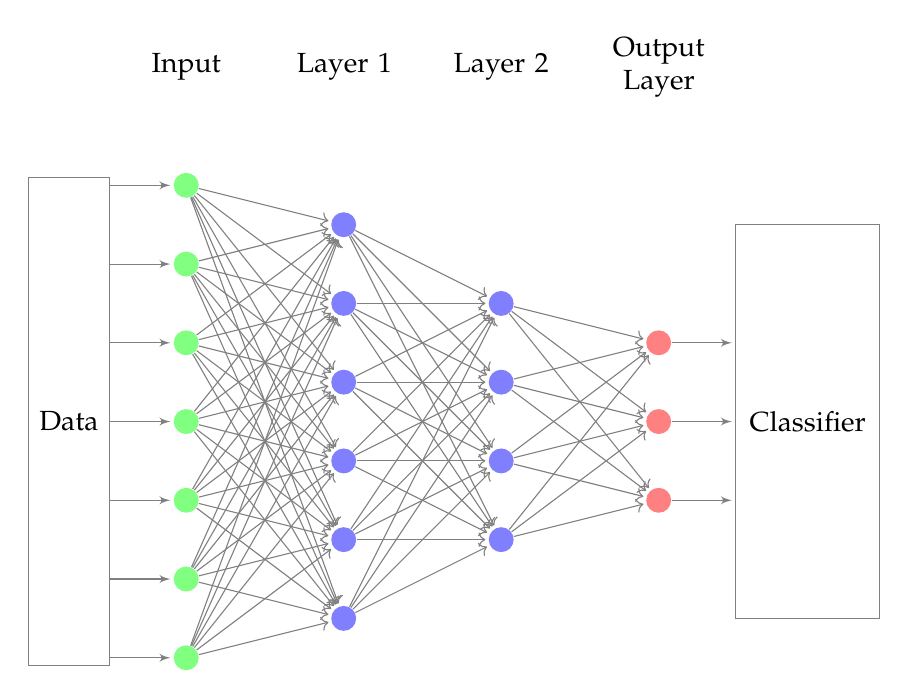
\begin{tikzpicture}[shorten >=1pt,->,draw=black!50, node distance=\layersep]
    \tikzstyle{every pin edge}=[<-,shorten <=1pt]
    \tikzstyle{neuron}=[circle,fill=black!25,minimum size=9pt,inner sep=0pt]
    \tikzstyle{input neuron}=[neuron, fill=green!50];
    \tikzstyle{output neuron}=[neuron, fill=red!50];
    \tikzstyle{hidden neuron}=[neuron, fill=blue!50];
    \tikzstyle{annot} = [text width=4em, text centered]

    % Draw the input layer nodes
    \foreach \name / \y in {1,...,7}
    % This is the same as writing \foreach \name / \y in {1/1,2/2,3/3,4/4}
        \node[input neuron] (I-\name) at (0,-\y) {};
%pin=left:Input \#\y
    % Draw the hidden layer nodes
    \foreach \name / \y in {1,...,6}
        \path[yshift=-0.5cm]
            node[hidden neuron] (H-\name) at (\layersep,-\y cm) {};

    \foreach \name / \y in {1,...,4}
        \path[yshift=-1.5cm,xshift=2.0cm]
            node[hidden neuron] (HH-\name) at (\layersep,-\y cm) {};

    \foreach \name / \y in {1,...,3}
        \path[yshift=-2cm,xshift=4.0cm]
            node[output neuron] (O-\name) at (\layersep,-\y cm) {};

    % Draw the output layer node
%   \foreach \name / \y in {1,...,3}
%        \path[yshift=-1.5cm,xshift=4.0cm]
%            \node[output neuron] (O-\name) at (\layersep,-\y cm) {};


    % Connect every node in the input layer with every node in the
    % hidden layer.
    \foreach \source in {1,...,7}
        \foreach \dest in {1,...,6}
            \path (I-\source) edge (H-\dest);

    \foreach \source in {1,...,6}
        \foreach \dest in {1,...,4}
            \path (H-\source) edge (HH-\dest);

    % Connect every node in the hidden layer with the output layer
    \foreach \source in {1,...,4}
        \foreach \dest in {1,...,3}
            \path (HH-\source) edge (O-\dest);

    % Annotate the layers
  \node [rectangle, draw, minimum height=6.2cm, text width=.8cm, text
  centered, left =.8cm of I-4] (mm) {Data};

    \foreach \source in {1,...,7}
        \path [line] (mm.east|-I-\source) -- (I-\source);

    \node[annot,above of=H-1, node distance=2cm] (hl) {Layer 1};
    \node[annot,left of=hl] {Input };
    \node[annot,right of=hl] (h3) {Layer 2} ;
    \node[annot,right of=h3] {Output Layer};
  \node [rectangle, draw, minimum height=5cm, text width=1.6cm, text
  centered, right =6.8cm of I-4] (mc) {Classifier};
    \foreach \source in {1,...,3}
        \path [line] (O-\source) -- (mc.west|-O-\source);


\end{tikzpicture}
}

%%%%%%%%%%%%%%%%%%%%%%%%%%%%%%%%%%%%%%%%%%%%%%%%%%%%%%%%%%%%%%%%

%%%%%%%%%%%%%%%%%%%%%%%%%%%%%%%%%%%%%%%%%%%(2)
% 2. define classifier

The output of this ANN is fed into a classifier. To complete this
example, we can define the most common classifier, Softmax:


\begin{definition}{Softmax (or the normalized exponential) is the function given by}
\[s : \R^n \to [0,1]^n\]
\[s_j(\vec x) = \frac{e^{x_j}}{\sum_{k = 1}^n e^{x_k}}\]
\end{definition}

\begin{definition}{We can define a classifier which picks the class corresponding with the largest output element from Softmax: }
\[\text{(Output Classification)  }   c_s(\vec x) = \text{argmax}_{i} s_i(\vec{x})\]
\end{definition}
% It is important that the classifier admit a directed error function
During training, the output $y \in \R^n$ from a network can thus be compressed using softmax into $[0,1]^n$ as a surrogate for probability for each possible class or directly into the classes which we can represent as the simplex for the vertices of $[0,1]^n$. 

\cite{Bishop:2006:PRM:1162264}

\subsubsection{Convolutional Neural Networks (CNNs)}\label{cnn}

Another common type of neural network which is a component in many modern applications including one in the experiments to follow are Convolutional Neural Networks (CNNs). CNNs are fundamentally composed of
perceptrons, but each layer is not fully connected to the
next. Instead, layers are arranged spatially and overlapping groups of perceptrons are independently connected to the nodes of the next layer, usually with a nonlinear filter that computes the maximum of all of the incoming nodes to a new node. This structure has been shown to be very effective on problems with spatial information \cite{lecun1995convolutional}. 

\subsection{Training ANNs}

Neural networks consist of a very large number of perceptrons with many parameters. Directly solving the system implied by these parameters and the empirical risk minimization problem defined below would be difficult, so we must use a
modular approach which takes advantage of the simple and regular structure of ANNs.

 A breakthrough came with the application of techniques derived from control theory to ANNs in the late 1980s \cite{rumelhart1986learning}, dubbed backpropagation. This technique was refined into its modern form in the thesis and continuing work of Yann LeCun \cite{lecun1988theoretical}. In this method, error is propagated backward taking advantage of the directed structure of the network to compute a gradient for each parameter defining it. Because modern ANNs are usually separated into discrete layers, gradients can be computed in parallel for all perceptrons at the same depth of the network
\cite{Bishop:2006:PRM:1162264}. Leveraging modern GPUs and parallel computing technologies, these gradients can be computed very quickly. There are a number of important considerations in training. We discuss a few in the following subsections. 

\subsubsection{Selection of the Training Set}

The first step in training an ANN is the selection of a training set. ANNs fundamentally are universal function approximators: Given a set of input data and corresponding output data, they approximate a mapping from one to the other. Performance is dependent on how well the phenomenon we hope to model is represented by the training data. The training data must consist of a set of inputs (e.g., images) and a set of outputs (e.g., labels) which contain sufficient examples to characterize the intended model. In a way, this is how we pose a question to the neural network. One must always ask whether the question we wish to pose is well-expressed by the training data we have available. 

The most important attributes of a training dataset are the number of
samples it contains and its density near where the model will be making predictions. According to conventional wisdom, training a neural network with $K$ parameters
will be very challenging if there are fewer than $K$ training samples
available. The modular structure of ANNs can be combined with regularization of the weights to overcome these limitations \cite{liu2015very}. 
In general, we will denote a training set by $(X,Y)$ where $X$ is an indexed set of inputs and $Y$ is a corresponding indexed set of labels. 

\subsubsection{Selecting a Loss Function}

Once we have selected a set of training data (both inputs and outputs), we must decide how we will evaluate the match between the ANNs output and the defined outputs from the training dataset -- we will quantify the deviation of the ANN compared with the given correspondence as a Loss. In general \emph{loss functions} are nonzero functions which compare an output $y$ against a ground-truth $\hat y$. Generally they have the property that an ideal outcome would have a loss of 0. 

One commonly used loss function for classification is known as Cross-Entropy Loss:
\begin{definition}{The Cross-Entropy Loss comparing two possible outputs is}
$L(y,\hat y) = -\sum_i y_i \log \hat y_i$.
\end{definition}
Other commonly used loss functions include $L^1$ loss (also referred to as Mean Absolute Error (MAE)), $L^2$ loss (often referred to as Mean-Squared-Error (MSE)), and Hinge Loss (also known as SVM loss). 

To set up the optimization, the loss for each training example must be aggregated. Generally, ANN training is conducted via Empirical Risk Minimization where Empirical Risk is defined for a given loss function $L$ as follows:
\begin{definition}{Given a loss function $L$, the Empirical Risk over a training dataset $(X,Y)$ of size $N$ is }
\[R_{\text{emp}}(P_{\vec w}(x) = \dfrac{1}{N} \sum_{(x,y) \in (X,Y)} L(P_{\vec w}(x)), y).\]
\end{definition}
We seek parameters $\vec w$ which will minimize $R_{\text{emp}}(P_{w}(x))$. This will be done with gradient-based optimization. 

\subsubsection{Computation of Gradient via Backpropagation}

Since it is relevant to the optimization being performed, we will briefly discuss the computation of gradients via backpropagation. For this discussion, we will introduce a small subset of a neural network in detail. In general, terms will be indexed as follows:
\[ x^{\text{[layer]}}_{\text{[node in layer], [node in previous layer]}}\]
When the second subscript is omitted, the subscript will only index the node in the current layer to which this element belongs. 

\scalebox{.9}{
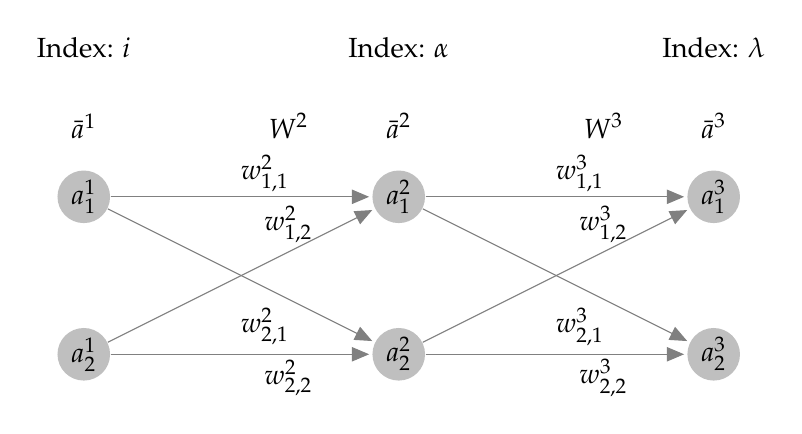
\begin{tikzpicture}[shorten >=1pt,->,draw=black!50, node distance=\layersep]

\node[circle, minimum size=19pt, fill=black!25, inner sep=0pt] (n11) at (0,2) {$a^1_1$};
\node[circle, minimum size=19pt, fill=black!25, inner sep=0pt] (n12) at (0,0) {$a^1_2$};
\node[circle, minimum size=19pt, fill=black!25, inner sep=0pt] (n21) at (4,2) {$a^2_1$};
\node[circle, minimum size=19pt, fill=black!25, inner sep=0pt] (n22) at (4,0) {$a^2_2$};
\node[circle, minimum size=19pt, fill=black!25, inner sep=0pt] (n31) at (8,2) {$a^3_1$};
\node[circle, minimum size=19pt, fill=black!25, inner sep=0pt] (n32) at (8,0) {$a^3_2$};

\node (av1) at (0,2.9) {$\Bar{a}^1$};
\node (av2) at (4,2.9) {$\Bar{a}^2$};
\node (av3) at (8,2.9) {$\Bar{a}^3$};

\node (ai1) at (0,3.9) {Index: $i$};
\node (ai2) at (4,3.9) {Index: $\alpha$};
\node (ai3) at (8,3.9) {Index: $\lambda$};

\node (w2) at (2.6,2.9) {$W^2$};
\node (w3) at (6.6,2.9) {$W^3$};


\draw[- triangle 45] (n11)  -- node[rotate=0,shift={(0.3,0.3)}] {$w^2_{1,1}$} (n21);
\draw[- triangle 45] (n11)  -- node[rotate=0,shift={(0.6,0.65)}] {$w^2_{1,2}$} (n22);
\draw[- triangle 45] (n12)  -- node[rotate=0,shift={(0.3,-0.65)}] {$w^2_{2,1}$} (n21);
\draw[- triangle 45] (n12)  -- node[rotate=0,shift={(0.6,-0.3)}] {$w^2_{2,2}$} (n22);

\draw[- triangle 45] (n21)  -- node[rotate=0,shift={(0.3,0.3)}]  {$w^3_{1,1}$} (n31);
\draw[- triangle 45] (n21)  -- node[rotate=0,shift={(0.6,0.65)}] {$w^3_{1,2}$} (n32);
\draw[- triangle 45] (n22)  -- node[rotate=0,shift={(0.3,-0.65)}]  {$w^3_{2,1}$} (n31);
\draw[- triangle 45] (n22)  -- node[rotate=0,shift={(0.6,-0.3)}]  {$w^3_{2,2}$} (n32);
\end{tikzpicture}
}

In this diagram, the $W^l$ are matrices composed of the weights indexed as above. Given an activation function for layer $n$ $A^n$ and its element-wise application to a vector $\bar A^n$, we can now write the output $\bar a_n$ for any layer of an arbitrary ANN in two ways \cite{Krause20}. Recursively, we can define
\begin{equation}
    a^n_\lambda = A^n(\sum_\alpha w^n_{\alpha, \lambda} a^{n-1}_\alpha)
\end{equation}
We can also write the matrix form of this recursion for every node in the layer:
\begin{equation}
\bar a^n = \bar A^n (W^n(\bar a^{n-1} ) )
\end{equation}
The matrix form makes it easier to write out a closed form for the output of the neural network. 
\begin{equation}
\bar a^n = \bar A^n (W^n(\bar A^{n-1}( W^{n-1} ( \cdots ( \bar A^{2} ( W^{2} \bar a^1) ) \cdots ) ) ) )
\end{equation}

Now, given a loss function $L = \sum_{i} \ell_i(a^n_i)$ where each $\ell_i$ is a loss function on the $i^{\text{th}}$ element of the output, we wish to compute the derivatives $\dfrac{\partial L}{\partial_{w^l_{i,j}}}$ for every $l, i,$ and $j$ which compose the gradient $\nabla L$. Using the diagram above, we can compute this directly for each weight using chain rule:
\begin{align*}
    \dfrac{\partial L}{\partial w^3_{\lambda,\alpha}} &= \dfrac{\partial L}{\partial a^3_{\lambda}} \dfrac{\partial a^3_{\lambda}}{\partial w^3_{\lambda,\alpha}} = \sum_{\lambda=1}^n \ell'_\lambda( a^3_\lambda) A'^3 (\sum_{\alpha=1}^n w^3_{\alpha, \lambda} a_\alpha^2) a^2_\alpha\\    
    %\dfrac{\partial L}{\partial w^2_{\alpha,i} } &= \sum_{\lambda} \dfrac{\partial L}{\partial a^3_{\lambda}} \dfrac{\partial a^3_{\lambda} }{\partial w^3_{\lambda,\alpha}} \dfrac{\partial a^2_\alpha }{ w^2_{\alpha,i}}\\
\end{align*}
Many of the terms of this gradient (e.g. the activations $a^n_i$ and the sums $\sum_{i} w^n_{i,j} a_i$) are computed during forward propagation when using the network to generate output. 
We will store such values during the forward pass and use a backward pass to fill in the rest of the gradient. Furthermore, notice that $\ell'_\lambda$ and $A'^n$ are well understood functions 
whose derivatives can be computed analytically almost everywhere. We can see that all of the partials will be of the form 
$\dfrac{\partial L}{\partial w^l_{n, i}} = \delta^l_n a^l_i$ where $\delta^l_n$  will contain terms which are either pre-computed or can be computed analytically. Conveniently, we can define this error signal recursively: 
\[
\delta^l_n = A'^l (a^l_{n}) \sum_{i = 1}^n w^{l+1}_{i, n} \delta^{l+1}_i
\]
In matrix form, we have
\[\bar \delta^l = \bar A'^l(W^l \bar a^l) \odot ((W^{l+1})^T \bar \delta^{l+1}\]
Where $\odot$ signifies element-wise multiplication. 

Then we can compute the gradient with respect to each layer's matrix $W^l$ as an outer product: 
\[\nabla_{W^l} L = \bar \delta^l \bar a^{(l-1)T}\]
Since this recursion for layer $n$ only requires information from layer $n+1$, this allows us to propagate the error signals that we compute backwards through the network. 


\subsubsection{Optimization of Weights}

Given a set of training input data and a method for computing gradients, our ultimate goal is to iteratively run our training-data through the network, updating weights gradually according to the gradients computed by backpropagation. In general, we start with some
default arrangement of the weights and choose a step
size $\eta$ for gradient descent. Then for each weight, in each iteration
of the learning algorithm, we apply a correction so that 
\[w'_{i',j',k'} = w_{i',j',k'}-\eta \frac{\partial E(Y,\hat Y)}{\partial
    w_{i',j',k'}}\]
    In this case, the step size (learning rate) $\eta$ is fixed throughout training.
    Numerical computation of the gradient requires first evaluating the network forward by computing the output for a given input. The value of every node in the network is saved and these values are used to weight the error as it is propagated backward through the network. Once the gradient is computed, the weights are adjusted according to the step defined above. This process is repeated until convergence is attained to within a tolerance. It should be
clear from the number of terms in this calculation that the initial
guess and step size can have significant effect on the eventual trained weights.
Due to lack of a guarantee for general convexity, poor guesses for such a large number of parameters can lead
to gradients blowing up or down   \cite{Bishop:2006:PRM:1162264}. 
. Due to nonlinearity and the plenitude of local minima in the loss function, classic gradient descent usually does not perform well during ANN training. \\ 
By far the most common technique for training the weights of neural networks adds noise in the form of random re-orderings of the training data to the general optimization process and is known as stochastic gradient descent. 
%\begin{tcolorbox}{}
\begin{definition}{Stochastic Gradient Descent (SGD)}

Given an ANN $N: \R^n \to C$, an initial set of weights for this network $\vec w_0$ (usually a small random perturbation from 0), a set of training data $X$ with labels $Y$, and a learning rate $\eta$, the algorithm is as follows: 

\begin{algorithm}
\caption*{Batch Stochastic Gradient Descent}\label{sgd}
\begin{algorithmic}[H]
\State $w = w_0$
\While{$E(\hat Y, P_w(X))$ (cumulative loss) is still improving} \Comment{ (the stopping condition may require that the weight change by less than $\e$ for some number of iterations or could be a fixed number of steps)}
\State Randomly shuffle $(X,Y)$
\State Draw a small batch $(\hat X, \hat Y) \subset (X, Y)$
\State $w \leftarrow w - \eta \left(\sum_{(x,y) \in (\hat X, \hat Y)}  \nabla L(P_w(\hat x), \hat y)\right)$
\EndWhile
\end{algorithmic}
\end{algorithm}
\end{definition}
%\end{tcolorbox}
Stochastic gradient descent achieves a smoothing effect on the gradient optimization by only sampling a subset of the training data for each iteration. Miraculously, this smoothing effect not only often achieves faster convergence, the result also generalizes better than solutions using deterministic gradient methods 
\cite{HardtRS15}. It is for this reason that SGD has been adopted as the de facto standard among ANN training applications.

\subsection{Adversarial Attacks }
%%%%%%%%%%%%%%%%%%%%%%%%%%%%%%%%%%%%%%%%%%%%%%%%%%%%%%%%%%%%%%(2)

In general \emph{Adversarial Attacks} against models
are small perturbations from natural data which significantly perturb
model output. 
Szegedy et al. \cite{Szegedy2013} realized that the same computational tools
used to train ANNs could be used to generate attacks that would
confuse them. Their approach was to define a loss function
relating the output of the ANN for a given initial image to a target adversarial 
output plus the $L^2$-norm of the input and use backpropagation to
compute gradients -- not on the weights of the neural network, but on
just the input layer to the network. The solution to this optimization
problem, efficiently approximated by a gradient-based optimizer, would
be a slightly perturbed natural input with a highly perturbed
output. Their experimental results are striking:\\

\begin{figure}[H]
    \centering
\includegraphics[width=7.3cm]{szegedy/negative1.png}\includegraphics[width=7.3cm]{szegedy/negative2.png}
    \caption{Natural Images are in columns 1 and 4, Adversarial images are in columns 3 and 6, and the difference between them (magnified by a factor of 10) is in columns 2 and 5. All images in columns 3 and 6 are classified by AlexNet as "Ostrich" \cite{Szegedy2013}}
    \label{fig:my_label}
\end{figure}

\subsubsection{Data Sets}

The Dataset used above is known as ImageNet -- a large set of labeled images varying in size originally compiled for the ImageNet Large Scale Visual Recognition Challenge (ILSVRC). This dataset and its many subsets has become a standard for image classification and feature identification experiments. In the experiments that follow, ImageNet will be featured alongside the Modified National Institute of Standards and Technology (MNIST) dataset which is a database of hand written digits often used to develop image processing and character recognition systems. This dataset is much lower resolution than ImageNet and is therefore experiments run much more quickly on it and require less complex input/output.  

\subsubsection{L-BFGS minimizing distortion}\label{lbfgs}

Szegedy et al. took advantage of the tools they had on hand for training neural networks to set up a box-constrained optimization problem whose approximated solution generates these targeted misclassifications. 


Let $f : \R^m \to \{1,...,k\}$ be a classifier and assume $f$ has an associated continuous loss function denoted by loss$_f : \R^m \times \{1,...,k\} \to \R^+$ and $l$ a target adversarial . \\
\textbf{ Minimize} $\Norm{r}_2$ subject to:
\begin{enumerate}[1.]
\item $f(x + r) = l$
\item $x + r \in [0,1]^m$
\end{enumerate}

The solution is approximated with L-BFGS (see Appendix \ref{appa}) as implemented in Pytorch or Keras. This technique yields examples that are close to their original counterparts in the $L^2$ sense.  \\

%Find the minimum $c > 0$ for which the minimizer $r$ of the following satisfies $f(x+r) = l$\\

%minimize $c|r| + $loss$_f(x+r,l)$ subject to $x + r \in [0,1]^m$.

\paragraph{L-BFGS: Mnist}
The following examples are prepared by implementing the above technique via pytorch on images from the Mnist dataset with FC200-200-10, a neural network with 2 hidden layers with 200 nodes each:
\begin{figure}[H]
\label{lbfgsa}
\includegraphics[trim=200 185 100 200, clip, width=7cm]{2019-04-10-adverse/mnist_examples/FC200-200-10-2448-O8-A0-attack_summary.png}\includegraphics[trim=200 185 100 200, clip,width=7cm]{2019-04-10-adverse/mnist_examples/FC200-200-10-2448-O8-A1-attack_summary.png}
\includegraphics[trim=200 185 100 200, clip,width=7cm]{2019-04-10-adverse/mnist_examples/FC200-200-10-2448-O8-A2-attack_summary.png}\includegraphics[trim=200 185 100 200, clip,width=7cm]{2019-04-10-adverse/mnist_examples/FC200-200-10-2448-O8-A3-attack_summary.png}
\includegraphics[trim=200 185 100 200, clip,width=7cm]{2019-04-10-adverse/mnist_examples/FC200-200-10-2448-O8-A4-attack_summary.png}\includegraphics[trim=200 185 100 200, clip,width=7cm]{2019-04-10-adverse/mnist_examples/FC200-200-10-2448-O8-A5-attack_summary.png}
\caption{Original images on the left, Perturbation is in the middle, Adversarial Image (total of Original with Perturbation) is on the right. Column 1 shows an original 8 being perturbed to adversarial classes 0, 2, and 4. Column 2 shows adversarial classes 1, 3, and 5}
\end{figure}
Borrowing a metric from Szegedy et al to compare the magnitude of these distortions, we will define
\begin{definition}{Distortion is the $L^2$ norm of the difference between an original image and a perturbed image, divided by the square root of the number of pixels in the image: }
\[\sqrt{\dfrac{\sum_i \hat (x_i - x_i)^2}{n}}\]
\end{definition}
Distortion is $L^2$ magnitude normalized by the square-root of the number of dimensions so that values can be compared for modeling problems with differing numbers of dimensions. 

The 900 examples generated for the network above had an average distortion of 0.089 with the following distribution of distortions, given in figure 3.

\begin{figure}[H]
\label{lbfgsh}
\includegraphics[trim=200 80 100 100, clip, width=16cm]{2019-04-10-adverse/mnist_examples/FC200-200-10-distortion_hist.png}
\caption{A histogram of the distortion measured for each of 900 adversarial examples generated using L-BFGS against the FC-200-200-10 network on Mnist. Mean distortion is 0.089.}
\end{figure}

\paragraph{L-BFGS: ImageNet}
\label{lbfgs-s}
We also tried to replicate \cite{Szegedy2013}'s results on ImageNet. Attacking VGG16, a well known model from the ILSVRC-2014 competition \cite{simonyan2014very}, on ImageNet images with the same technique generates the examples in figure 4: 

\begin{figure}[H]
\label{lbfgsis}
\includegraphics[trim=200 185 100 200, clip, width=8cm]{2019-04-10-adverse/imnet_examples/vgg16-ILSVRC2012_val_00039098-O722-A965-attack_summary.png}\includegraphics[trim=200 185 100 200, clip, width=8cm]{2019-04-10-adverse/imnet_examples/vgg16-ILSVRC2012_val_00027142-O52-A347-attack_summary.png}
\includegraphics[trim=200 185 100 200, clip, width=8cm]{2019-04-10-adverse/imnet_examples/vgg16-ILSVRC2012_val_00029901-O425-A468-attack_summary.png}\includegraphics[trim=200 185 100 200, clip, width=8cm]{2019-04-10-adverse/imnet_examples/ILSVRC2012_val_00001375-Otensor([42])-A694-attack_summary.png}
% \includegraphics[width=7cm]{2019-04-10-adverse/imnet_examples/vgg16-ILSVRC2012_val_00035978-O803-A353-attack_summary.png}
% \includegraphics[width=7cm]{2019-04-10-adverse/imnet_examples/ILSVRC2012_val_00000886-Otensor([940])-A684-attack_summary.png}
\caption{Original images on the left, Perturbation (magnified by a factor of 100) by is in the middle, Adversarial Image (total of Original with Perturbation) is on the right. }
\end{figure}

%The average distortion was 0.01 distributed as seen in figure \ref{lbfgsi}. 

\begin{figure}[H]
\label{lbfgsi}
\includegraphics[trim=200 80 100 100, clip,width=14cm]{2019-04-10-adverse/imnet_examples/distortion_hist.png}
\caption{A histogram of the distortion measured for each of 112 adversarial examples generated using L-BFGS against the VGG16 network on ImageNet images with mean distortion 0.0107}
\end{figure}

\paragraph{Fast Gradient Sign Method (FGSM)} 

  We also implemented a single step attack process uses the gradient of the loss function $L$ with respect to the image to find the adversarial perturbation \cite{goodfellow_explaining_2014}. for given $\e$, the modified image $\hat x$ is computed as
\begin{equation}
\hat{x} = x + \epsilon \text{sign} (\nabla L (P_w(x),x))
\end{equation}

This method is simpler and much faster to compute than the L-BFGS technique described above, but produces adversarial examples less reliably and with generally larger distortion. Performance was similar but inferior to the Iterative Gradient Sign Method summarized below.  
%\[\hat x = x + \e \sign(\Delta \ell(F(x'_m),x'_m))\]

\paragraph{Iterative Gradient Sign Method (IGSM)}
\label{igsm-s}
In \cite{kurakin_adversarial_2016}
  an iterative application of FGSM was proposed. After each
  iteration, the image is clipped to a $\e L_\infty$ neighborhood of the original. Let $x'_0 = x$, then after $m$ iterations, the adversarial image obtained is:
\begin{equation}
x_{m+1}' = \text{Clip}_{x,\epsilon} \Bigl\{x_m' + \alpha \times \text{sign}(\nabla \ell (F(x'_m),x'_m))  \Bigr\} 
\label{igsm}
\end{equation}
This method is faster than L-BFGS and more reliable than FGSM but still produces examples with greater distortion than L-BFGS. 
%  \[x'_{m + 1} = \text{Clip}_{x,\e} \{ x'_m + \alpha \times
%  \sign(\Delta \ell(F(x'_m),x'_m))\] 
\begin{figure}[H]
  \centering
\includegraphics[trim=200 110 1200 102, clip,width=4cm]{2019-04-10-adverse/ILSVRC2012_val_00002900summary_plot.png}\includegraphics[trim=900 110 500 102, clip,width=4cm]{2019-04-10-adverse/ILSVRC2012_val_00002900summary_plot.png}
%\includegraphics[width=12cm]{2019-04-10-adverse/ILSVRC2012_val_00048234summary_plot.png}
\caption{adversarial example generated against VGG16 (ImageNet) with IGSM. Original Image on the left, adversarial image and added noise (ratio of variance adversarial noise/original image: 0.0000999) on the right. }
\label{fgsmhip}
\end{figure}

%The attacks contained in figure ~\ref{fgsmhip} were generated with IGSM against VGG16


\subsubsection{Other Attacks}
The following attack techniques are also prevalent in the literature but have not been replicated in these experiments. 

\paragraph{Jacobian-based Saliency Map Attack (JSMA)} Another attack noted by  \cite{papernot_limitations_2015}
  estimates the \emph{saliency map}, a rating for each of the input features (e.g. each pixel) on how influential it is for causing the model to predict a particular class with respect to the model output \cite{wiyatno2018saliency}. This attack modifies the pixels that are most salient. This is a targeted attack, and saliency is designed to find the pixel which increases the classifier's output for the target class while tending to decrease the output for other classes.

\paragraph{Deep Fool (DFool)} A technique proposed by \cite{moosavi-dezfooli_deepfool:_2015}
  to generate an un-targeted iterative attack. 
This method approximates the classifier as a linear decision boundary and then finds the smallest perturbation needed to cross that boundary.
This attack minimizes $L_2$ norm with respect to  to the original image.

\paragraph{Carlini \& Wagner (C\&W)} In \cite{carlini_towards_2016}
  an adversarial attack is proposed which updates the loss function such that it jointly minimizes $L_p$ and a custom differentiable loss function based on un-normalized outputs of the classifier (\textit{logits}). 
Let $Z_k$ denote the logits of a model for a given class $k$, and $\kappa$ a margin parameter. Then C\&W tries to minimize:
\begin{equation}
|| x - \hat{x} ||_p + c* max\left(Z_k(\hat{x}_y) - max\{Z_k(\hat{x}) : k \neq y\},-\kappa\right)
\end{equation}

\part{Persistence}

\section{Introduction}


Deep Neural Networks (DNNs) and their variants are core to the success of modern machine learning \cite{prakash2018}, and have dominated competitions in image processing, optical character recognition, object detection, video classification, natural language processing, and many other fields ~\cite{SCHMIDHUBER201585}. Yet such classifiers are notoriously susceptible to manipulation via adversarial examples \cite{Szegedy2013}. Adversarial examples occur when natural data are close enough to the decision boundary that they can be imperceptibly perturbed to another class. Adversarial examples are not just a peculiarity, but seem to occur for most, if not all, DNN classifiers. For example, ~\cite{shafahi2018are} used isoperimetric inequalities on high dimensional spheres and hypercubes to conclude that there is a reasonably high probability that a correctly classified data point has a nearby adversarial example. ~\cite{ilyas2019adversarial} showed that adversarial examples can arise from features that are good for classification but not robust to perturbation.

%There are now a wide variety of attacks which produce adversarial examples and defenses which try to detect them. \todo{[DG]: not sure this is necessary. [K]: This paragraph is incomplete. Do you think there shouldn't be such a paragraph at all? [DG]: Not sure it is needed. If so, it maybe should probably come right at the beginning before the shafahi/are adversarial examples inevitable.}

There have been many attempts to identify adversarial examples using properties of the decision boundary. ~\cite{Fawzi2018empirical} found that decision boundaries tend to have highly curved regions, and these regions tend to favor negative curvature, indicating that regions that define classes are highly nonconvex. These were found for a variety of DNNs and classification tasks. 
%They also suggest exploiting this curvature discrepancy to identify when a data point is a natural image and when it is adversarial. 
A related idea is that adversarial examples often arise within cones, outside of which images are classified in the original class, as observed by ~\cite{roth19aodds}. Many theoretical models of adversarial examples, for instance the dimple model developed by ~\cite{shamir2021}, have high curvature and/or sharp corners as an essential piece of why adversarial examples can exists very close to natural examples.



{\bf Contributions.} We propose two concepts, $(\gamma,\sigma)$-stability and $\gamma$-persistence.  Both are defined with reference to a classifier and a given point (which can be either a natural or adversarial image, for example). The proposed notion of stability is more nuanced than simply measuring distance to the decision boundary, and is also capable of elucidating information about the curvature of the nearby decision boundary.  Persistence is a statistic that measures how far away from a point one can go via Gaussian sampling and still consistently find points with the same classification. One advantage of this statistic is that it is easily estimated by sending a Monte Carlo sampling about the point through the classifier.


% Deep Neural Networks (DNNs) and other optimization-based
% function approximation models are the core of modern
% machine learning \cite{prakash2018}. These models have   {\color{red}All such modern models are
% trained via gradient-based optimization, e.g. Stochastic Gradient Descent (SGD) with
% gradients computed via back propagation ~\cite{goodfellow2013multidigit}.} \todo{[K]: I suggest taking out this red sentence.} Although the performance of these models is practically
% miraculous within the training and testing context for which they are designed, they remain very susceptible to attacks. It was discovered by
% ~\cite{Szegedy2013} that images can be generated
% which apparently trick such models in a classification context in  difficult-to-control ways ~\cite{Khoury2018}. The intent of this
% research is to investigate these \emph{adversarial examples} in a
% mathematical context and use them to study pertinent 
% properties of the learning models from which they arise.\todo{[K]: Make last sentence stronger/more punchy. [DG]: This whole paragraph needs significant work and should read a little more like the abstract, maybe.}

%\section{Prior Work (update title)}
%\subsection{On Adaptive Attacks to Adversarial Example Defenses}
%wTramer et al present methodology and approach necessary to perform adaptive attacks against defended neural networks \cite{tramer2020adaptive}. 

% notes: page 4 claims their methods are "consistent" so that higher loss values result in strictly stronger attacks -- higher? isn't the idea to minimize loss values? In what context is higher better?
%  
%94

% ~\cite{Khoury2018} suggest that a classifier is robust if the class of each point in the data manifold is contained in a sufficiently large ball that is entirely contained in the same class. The larger the ball, the more robust the classifier. ~\cite{gilmer2018adversarial} use the average distance to the nearest error\todo{[K]: Error? is it accurate to say "erroniously classified point"? [DG]: What they mean in this paper is the distance to the nearest class that is different} to capture robustness, and then show an example where an accurate classifier results in a small distance to the nearest error. 

% ~\cite{shafahi2018are} use isoperimetric inequalities on high dimensional spheres and hypercubes to conclude that there is a reasonable probability that a correctly classified data point has a nearby adversarial example.

% ~\cite{Fawzi2018empirical} found that decision boundaries tend to have highly curved regions, and these regions tend to favor negative curvature, indicating that regions that define classes are highly nonconvex. These were found for a variety of DNNs and classification tasks. They also suggest exploiting this curvature discrepency to identify when a data point is a natural image and when it is adversarial. Our methods try to exploit similar structure, but is done in a different way by doing Gaussian sampling about a point instead of approximating curvatures of decision boundaries. Since the results in \cite{Fawzi2018empirical} are based on computing an approximation of a curvature function, they depend on an assumption of being close to the decision boundary. Our method does not need that assumption since the Gaussian sampling is not related to functions but instead based on measures. Curvatures have a close connection to tube formulas \cite{morvan}, which is related to the uniform measure on balls. These measures may not be well-behaved in high dimensions, which is one of the main reasons we choose to instead consider Gaussian measures, which factorize nicely in high dimensions.
% \todo{[DG]: These need to be expanded and placed here or elsewhere, but are extremely important.}

% \section{Background}\todo{[DG]: probably remove this whole section}
% %%%%%%%%%%%%%%%%%%%%%%%%%%%%%%%%%%%%%%%%%%%%%%%%%%%%%%%%%%%%%%(2)

% We primarily consider adversarial examples for classifiers.  To wit, let $X$ be a set of possible data and let $L$ be a set of labels. We will consider classifier as a map $\CC: X \to L$. In general $X$ may be much larger than the actual space from which our data are drawn. If the data actually come from a submanifold of $X$, we call this the \emph{data submanifold}. The data submanifold may not be a strict submanifold, and we often do not know the shape or even dimension of it.

% %Data is drawn from a distribution $\mu$ on $X$ that is usually not known. The overarching goal of classification is to produce a classifier such that $\CC$ is as good as possible on the support of $\mu$. 
% %We define $X_N \subseteq X$ to be the support of $\mu$ and call it the set of \emph{natural data}. 
% %Usually our classification problem is the following: given a set of i.i.d. samples $\Sigma \sim \mu$
% %, where we consider $\Sigma \subseteq X_N$, 
% %and a classifier $\CC_\Sigma$ on $\Sigma$, find a classifier $\CC$ on $X$ such that $\CC$ lies in some class of ``good functions'' in such a way that it is relatively good at interpolating and/or extrapolating $\CC_\Sigma$. In particular, we hope that $\CC$ is as accurate as possible on the support of $\mu$, which we call the ``natural data.'' \todo{[K]: To a ML audience, it seems to me a bit overkill to describe the idea of statistical learning. Also, this isn't how they would likely describe it, so it could put people off. DG: Agreed, we can probably eliminate this.}
% The classifier $\CC$ partitions $X$ into classes, each of which is defined as $\CC^{-1}(\ell)$ for some $\ell \in L$. Points on the boundaries of these classes do not have a clear choice of label, and the points in $X$ on the boundaries of the classes make up the \emph{decision boundary} for $\CC$.

% %To build up to a definition for stability, we develop definitions and terms to refer to adversarial examples without relying on subjective characteristics like human vision. 
% %Let $X$ denote a set of possible data and $L$ denote a set of labels that distinguish the different classes. 
% We are now ready to define adversarial examples.%We now define adversarial examples.

% \begin{definition} \label{def:advers}
% Let $d$ be a metric on $X$, let $x\in X$ have label $\ell\in L$, and let $\CC:X\to L$ be a classifier.  We say that $x$ admits an \emph{$(\e,d)$--adversarial example} to $\CC$ if there exists $\hat x \in X$ such that $d(x,\hat x) < \e$ and $\CC(\hat x) \neq \ell$.
% %Consider a point $x \in X$ with corresponding class $\ell \in C$ and a classifier $\CC: X \to C$. We say that $x$ admits an \emph{$(\e,d)-$adversarial example} on $\CC$ if there exists a point $\hat x$ such that $d(x,\hat x) < \e$ and $\CC(\hat x) \neq c$. 
% \end{definition}
% One typically considers Definition \ref{def:advers} in the context of small $\e$. 
% %Often consideration is made of when such a misclassification is a result of an intentionally act by an adversary. 
% There are various methods of producing adversarial examples which are discussed later. In some cases, the adversarial label is explicitly targeted:
% \begin{definition}
% Let $d$ be a metric on $X$, let $x\in X$ have label $\ell\in L$, and let $\CC:X\to L$ be a classifier.  Let $\varepsilon>0$ and $\ell_t\neq \ell$ be fixed but arbitrary. We say that $x$ admits an \emph{$(\varepsilon,d,\ell_t)$--targeted adversarial example} to $\mathcal{C}$ if there exists $\hat{x}\in X$ such that $d(x,\hat{x})<\varepsilon$ and $\CC(\hat{x})=\ell_t$.
% %Consider a point $x \in X$ with corresponding class $\ell \in C$ and a classifier $\CC: X \to C$. We say that $x$ admits an \emph{$(\e,d,\ell_t)-$targeted adversarial example} on $\CC$ if there exists a point $\hat x$ such that $d(x,\hat x) < \e$ and $\CC(\hat x) = \ell_t$. 
% \end{definition}

% These definitions rely on a metric $d$, emphasizing the reliance on the choice of distance to understand notions of closeness. From here on, we will assume that $(X,d)$ is a Euclidean vector space with $d$ being the Euclidean metric. This will allow for the use of standard Gaussian distributions as well.\todo{[K]: The part about Gaussians here is unclear. [DG]: What I mean here is that one needs a distance metric to define Gaussian distributions. Maybe it is not relevant here?}


% Note that there is no restriction on whether adversarial examples come from the set of natural examples, and typically we will assume that they do not so that we can draw a contrast. 
% %We define adversarial examples, sometimes called adversarial attacks, against classifiers
% %to be small perturbations from natural data that significantly change the classifier output. See Definition \ref{def:advers} for a formal definition.
% %Szegedy et al. 
% ~\cite{Szegedy2013} realized that the same computational tools
% used to train DNN classifiers could be used to generate attacks that would
% confuse them. Their approach was to define a loss function
% relating the output of the DNN for a given initial image to a target adversarial 
% output plus the $L^2$-norm of the input and use backpropagation to 
% compute gradients -- not on the weights of the neural network, but on
% just the input layer to the network. The solution to this optimization
% problem, efficiently approximated by a gradient-based optimizer, would
% be a slightly perturbed natural input with a highly perturbed
% output. There has since been significant work describing methods of producing and identifying
% adversarial examples. In the next sections, we describe some of the most relevant
% to our work here.

% %Their experimental results are striking:\\

% %\begin{figure}[t]
% %    \centering
% %\includegraphics[width=7.3cm]{szegedy/negative1.png}\includegraphics[width=7.3cm]{szegedy/negative2.png}
% %    \caption{Natural Images are in columns 1 and 4, Adversarial images are in columns 3 and 6, and the difference between them (magnified by a factor of 10) is in columns 2 and 5. All images in columns 3 and 6 are classified by AlexNet as "Ostrich" \cite{Szegedy2013}}
% %    \label{fig:my_label}
% %\end{figure}



% %The Dataset used above is known as ImageNet -- a large set of labeled images varying in size originally compiled for the ImageNet Large Scale Visual Recognition Challenge (ILSVRC). This dataset and its many subsets has become a standard for image classification and feature identification experiments. In the experiments that follow, ImageNet will be featured alongside the Modified National Institute of Standards and Technology (MNIST) dataset which is a database of hand written digits often used to develop image processing and character recognition systems. This dataset is much lower resolution than ImageNet and is therefore experiments run much more quickly on it and require less complex input/output.  

\section{Motivation and related work}
Our work is intended to shed light on the existence and prevalence of adversarial examples to DNN classifiers. It is closely related to other attempts to characterize robustness to adversarial perturbations, and here we give a detailed comparison.


%In the Sections \ref{sec:stab} and \ref{sec:experiments}, we will investigate stability of both natural data and adversarial examples in an attempt to understand how these different sets lie in the domain of the classifier. Understanding these geometries is a challenge for several reasons. For one, the data lies in a high dimensional space and thus the decision boundaries between classes are complicated submanifolds. Distances in high dimensional spaces are difficult to work with and do not always yield useful information. In particular, uniform distributions on balls in high dimensions often result in surprising results ~\cite{aggsurprising}. Instead, we consider high dimensional Gaussian distributions, using the variance as an alternative to distance. ~\cite{roth19aodds} and ~\cite{hosseini2019odds} take a similar approach, considering Gaussian noise perturbations of $\varepsilon$ times a vector with normal distribution $N(0,I)$. We describe their work below but note that they do not take advantage of using the variance to probe distributions which are more or less concentrated near their means.


%DG: moved to introduction Adversarial examples occur when natural data are close enough to the decision boundary that they can be imperceptibly perturbed to another class. Adversarial examples are not just a peculiarity, but seem to occur for most if not all DNN classifiers. ~\cite{shafahi2018are} use isoperimetric inequalities on high dimensional spheres and hypercubes to conclude that there is a reasonably high probability that a correctly classified data point has a nearby adversarial example. ~\cite{ilyas2019adversarial} show that adversarial examples can arise from features that are good for classification but not robust to perturbation.

%{\bf Properties of the decision boundary.}
%data manifold, curvature of the decision boundary

{\bf Distance-based robustness.}
%Since we expect adversarial examples to exist, an important question is whether we can define a classifier to be robust to perturbations that might shift a natural example to an adversarial example. 
A typical approach to robustness of a classifier is to consider distances from the data manifold to the decision boundary.  ~\cite{Khoury2018} define a classifier to be robust if the class of each point in the data manifold is contained in a sufficiently large ball that is entirely contained in the same class. The larger the balls, the more robust the classifier. It is then shown that if training sets are sufficiently dense in relation to the reach of the decision axis, the classifier will be robust in the sense that it classifies nearby points correctly. In practice, we do not know that the data is so well-positioned, and it is quite possible, especially in high dimensions, that the reach is extremely small, as evidenced by results on the prevalence of adversarial examples, e.g., \cite{shafahi2018are}.

~\cite{tsipras2018robustness} investigated robustness in terms of how small perturbations affect the the average loss of a classifier. They define standard accuracy of a classifier in terms of how often it classifies correctly, and robust accuracy in terms of how often an adversarially perturbed example classifies correctly. It was shown that sometimes accuracy of a classifier can result in poor robust accuracy. ~\cite{gilmer2018adversarial} use the expected distance to the nearest different class (when drawing a data point from the data distribution) to capture robustness, and then show that an accurate classifier can result in a small distance to the nearest different class in high dimensions when the data is drawn from concentric spheres. 

{\bf Adversarial detection via sampling.}
While adversarial examples often occur, they still may be rare in the sense that most perturbations do not produce adversarial examples. ~\cite{yu2019new} used the observation that adversarial examples are both rare and close to the decision boundary to detect adversarial examples. They take a potential data point and look to see if nearby data points are classified differently than the original data point after only a few iterations of a gradient descent algorithm. If this is true, the data point is likely natural and if not, it is likely adversarial. We will draw on a similar idea by considering nearby points drawn from Gaussian distributions of varying standard deviations in order to better quantify this observation of rarity. In general, the results of ~\cite{yu2019new} indicate that considering samples of nearby points, which approximate the computation of integrals, is likely to be more successful than methods that consider only distance to the decision boundary.

%The goal would be to either develop a classifier robust to adversarial examples or to identify adversarial examples as opposed to natural data.

%DG: Moved to introduction. There have been many attempts to identify adversarial examples using properties of the decision boundary. ~\cite{Fawzi2018empirical} found that decision boundaries tend to have highly curved regions, and these regions tend to favor negative curvature, indicating that regions that define classes are highly nonconvex. These were found for a variety of DNNs and classification tasks. They also suggest exploiting this curvature discrepancy to identify when a data point is a natural image and when it is adversarial. It is also suggested that adversairal examples often arise within a cone, outside of which images are classified in the original class, as observed by ~\cite{roth19aodds} and as part of the dimple model theorized by ~\cite{shamir2021}.



~\cite{roth19aodds} proposed a statistical method to identify adversarial examples from natural data. Their main idea was to consider how the last layer in the neural network (the logit layer) would behave on small perturbations of a natural example. %, i.e., on $x+\varepsilon n$ where $x$ is a natural example, $\varepsilon>0$ is small, and $n \sim N(0,I)$.  
This is then compared to the behavior of a potential adversarial example. If it differs by a predetermined threshold, the example is flagged as adversarial. Successfully flagging adversarial examples in this way works best when adversarial examples tend to perturb toward the original class from which the adversarial example was perturbed. However, this is not always the case.
It was shown by ~\cite{hosseini2019odds} that it is possible to produce adversarial examples, for instance using a logit mimicry attack, that instead of perturbing an adversarial example toward the true class, actually perturb to some other background class. In fact, we will see in Section \ref{sec:mnist} that the emergence of a background class, which was observed as well by ~\cite{roth19aodds}, is quite common. 

%DG: Mostly moved to introduction. ~\cite{roth19aodds} propose a statistical method to identify adversarial examples from natural data. Their main idea is to consider how the last layer in the neural network (the logit layer) would behave on a natural example with a small Gaussian perturbation, i.e., on $x+\varepsilon n$ where $x$ is a natural example, $\varepsilon>0$ is small, and $n \sim N(0,I)$.  This is then compared to the behavior of a potential adversarial example. If it differs by a predetermined threshold, the example is flagged as adversarial. Successfully flagging adversarial examples in this way is predicated on the hypothesis that adversarial examples tend to perturb toward the true class that they have been perturbed from. It is shown by ~\cite{hosseini2019odds} that it is possible to produce adversarial examples, for instance using a logit mimicry attack, that instead of perturbing an adversarial example toward the true class, actually perturb to some other background class. 
%In fact, we will see in Section \ref{sec:mnist} that the emergence of a background class, which was observed as well by ~\cite{roth19aodds}, is quite common. 

%This behavior will be observed in the case of classifiers of the MNIST digits dataset.

Whereas ~\cite{roth19aodds} consider adding various types of noise to a given point and ~\cite{hosseini2019odds} consider small Gaussian perturbations of $x$ sampled from $N(x,\varepsilon^2 I)$ for small $\varepsilon$, %\todo{[K]: Should we go ahead and just be clear here and say $N(x,\varepsilon^2 I)$?} %noise perturbations of $\varepsilon$ times a vector with normal distribution $N(0,I)$ with a small selection of choices for $\varepsilon.$
we specifically focus on %Our choice to consider varying standard deviations is quite similar to considering varying choices of $\varepsilon$ in the latter, but our focus is on 
tuning the standard deviation parameter to determine a statistic describing how a given data point is placed within its class. The $\gamma$-persistence then gives a measurement similar to distance to the boundary but that is drawn from sampling instead of distance. The sampling allows for a better description of the local geometry of the class and decision boundary, as we will see in Section \ref{sec:stab}. Our statistic is based on the fraction of a Gaussian sampling of the neighborhood of a point which receives the same classification; this is different from that of ~\cite{roth19aodds}, which is the expected difference of the output of the logit layer of the original data point and the output of the logit layer for perturbed data points.  Additionally, while their statistics are defined pairwise with reference to pre-chosen original and candidate classes, ours is not.


%The focus of this particular paper is choosing that length apprWe instead consider perturbations of the form $N(0,\sigma^2 I)$ and vary $\sigma$. Each of these methods will perturbations with the same average length if $\varepsilon=\sigma$, but the latter will provide a greater spread of values for the length of the perturbations.

%The main reason\todo{[DG]: Yes, this needs to be moved. [K]: Yeah, but they are using Gaussians too, so I don't understand this comment about uniform distributions..} is that high dimensional Gaussian distributions are generally better behaved than uniform distributions on balls in high dimensions ~\cite{aggsurprising}. In addition, instead of just testing for various choices of the parameter, we find the parameter value for which the expectation of having a different result is above a certain threshold.

% ~\cite{yu2019new} observed that adversarial examples are a problem both because many are close to the decision boundary and they are rare. They use these almost contradictory observations to detect adversarial examples by taking a potential datapoint and looking to see if there are contra-classfied points (i.e., points classified different than the original datapoint) nearby that can be reached by only a few iterations of a gradient descent algorithm. If this is true, the datapoint is likely natural and if not, it is likely adversarial. The algorithm uses cutoff points based on previous understanding of the data. 



%Each of these works is predicated on understanding stability of natural and adversarial examples under Gaussian perturbations of the data. In this study, we look more closely at how such perturbations change classification. In the sequel, we will give a definition that is agnostic of choice of classifier, though we focus on different types of Neural Network based classifiers.

{\bf Summary.}
 In Sections \ref{sec:stab} and \ref{sec:experiments}, we will investigate stability of both natural data and adversarial examples by considering sampling from Gaussian distributions centered at a data point with varying standard deviations. Using the standard deviation as a parameter, we are able to derive a statistic for each point that captures how entrenched it is in its class in a way that is less restrictive than the robustness described by ~\cite{Khoury2018}, takes into account the rareness of adversarial examples described by ~\cite{yu2019new}, builds on the idea of sampling described by ~\cite{roth19aodds} and ~\cite{hosseini2019odds}, and represent curvatures in a sense related to ~\cite{Fawzi2018empirical}. 
 %The main contribution is the development of a precise notion of stability, called $(\gamma, \sigma)$-stability, and a statistic, called $\gamma$-persistence, that represent each of these notions in a quantitative, clear way. The methods use sampling of Gaussians, which is generally quite easy compared to other measures in high dimensions.  \todo{[DG]: we maybe want to add the reference \cite{creschi2019} to discuss using dimension reduction/t-SNE to capture manifold property of data and \cite{Lee2018ASU} with a method to detect out of manifold data for adversarial attacks} 


\section{Stability and Persistence} \label{sec:stab}
In this section we define a notion of stability of classification of a point under a given classification model. In the following, $X$ represents the ambient space the data is drawn from (typically $\RR^n$) even if the data lives on a submanifold of $X$, and $L$ is a set of labels (often $\{1,\dots,\ell\}$).  Note that points $x\in X$ can be natural or adversarial points.%The following definition complements the definition for adversarial examples by providing a criteria for the local stability of the classifier about a point, which could be an actual test point or an adversarial example: 

\begin{definition}
Let $\CC:X\to L$ be a classifier, $x \in X$, $\gamma\in(0,1)$, and $\sigma>0$. We say $x$ is \emph{$(\gamma,\sigma)$-stable} with respect to $\CC$ if $\mathbb{P}[\CC(x')=\CC(x)] \geq \gamma$ for $x' \sim \rho = N(x, \sigma^2 I)$; i.e. $x'$ is drawn from a Gaussian with variance $\sigma^2$ and mean $x$.
\end{definition}

In the common setting when $X=\RR^n$, we have
\[\mathbb{P}[\CC(x')=\CC(x)] = \int_{\RR^n} \mathbbm{1}_{\CC^{-1}(\CC(x))} (x') d\rho (x') = \rho(\CC^{-1}\CC(x)).\]
Note here that $\CC^{-1}$ denotes preimage. %In the case of images drawn from $\RR^n$, we can write this integral precisely as
One could substitute various probability measures $\rho$ above with mean $x$ and variance $\sigma^2$ to obtain different measures of stability corresponding to different ways of sampling the neighborhood of a point.  Another natural choice would be sampling the uniform measure on balls of changing radius. Based on the concentration of measure for both of these families of measures (see Appendix \ref{sec:concentration}), we do not anticipate significant qualitative differences in these two approaches. We propose Gaussian sampling because it is also a product measure, which makes it easier to sample and simplifies some other calculations below.

For the Gaussian measure, the probability above may be written more concretely as
\begin{equation}\label{EQN:Gaussian}
\frac{1}{\left(\sqrt{2\pi}\sigma\right)^{n}} \int_{\RR^n} \mathbbm{1}_{\CC^{-1}(\CC(x))} (x')e^{-\frac{\norm{x - x'}^2}{2\sigma^2}} dx'.
\end{equation}
In this work, we will conduct experiments in which we estimate this stability for fixed $(\gamma,\sigma)$ pairs via a Monte Carlo sampling, in which case the integral \eqref{EQN:Gaussian} is approximated by taking $N$ i.i.d. samples $x_k \sim \rho$ and computing
\[
    \frac{\norm{x_k : \CC(x_k) = \CC(x)}}{N}.
\]
Note that this quantity converges to the integral \eqref{EQN:Gaussian} as $N\to\infty$ by the Law of Large Numbers.

The ability to adjust the quantity $\gamma$ is important because it is much weaker than a notion of stability that requires a ball that stays away from the decision boundary as in \cite{Khoury2018}. By choosing $\gamma$ closer to $1$, we can require the samples to be more within the same class, and by adjusting $\gamma$ to be smaller we can allow more overlap.

We also propose a related statistic, \emph{persistence}, by fixing a particular $\gamma$ and adjusting $\sigma$. For any $x\in X$ not on the decision boundary, for any choice of $0<\gamma<1$ there exists a $\sigma_\gamma$ small enough such that if $\sigma < \sigma_\gamma$ then $x$ is $(\gamma,\sigma)$-stable. We can now take the largest such $\sigma_\gamma$ to define persistence.

%In our experiments, $\gamma$ is fixed and $\sigma$ is adjusted to determine the largest $\sigma$ for which an image is $(\gamma,\sigma)$-stable.  We define this to be persistence as follows.


\begin{definition}
    Let $\CC:X\to L$ be a classifier, $x \in X$, and $\gamma\in(0,1)$. Let $\sigma_\gamma^*$ be the maximum $\sigma_\gamma$ such that $x$ is $(\gamma, \sigma)$-stable with respect to $\CC$ for all $\sigma<\sigma_\gamma$. We say that $x$ has \emph{$\gamma$-persistence} $\sigma_\gamma^*$.
\end{definition}

The $\gamma$-persistence quantity $\sigma_\gamma^*$ measures the stability of the neighborhood of a given $x$ with respect to the output classification. Small persistence indicates that the classifier is unstable in a small neighborhood of $x$, whereas large persistence indicates stability of the classifier in a small neighborhood of $x$. In the later experiments, we have generally taken $\gamma = 0.7$. This choice is arbitrary and chosen to fit the problems considered here. In our experiments, we did not see significant change in results with small changes in the choice of $\gamma$.

In order to better understand the notion of $\gamma$-persistence, consider a decision boundary that is the boundary of a conical wedge domain $W^n_k \subset \RR^n$, where $0<k\leq n$, defined by 
\[
    W^n_k = \{(x_1, \ldots, x_n) \in \RR^n : x_1 \geq 0, \ldots, x_k \geq 0\}.
\]
One can consider this as a Cartesian product of a half space and a positive orthant (see Figure \ref{fig:orthants} for the three possibilities if $n=3$). The boundary of $W^n_k$ consists of parts of hyperplanes (in fact, $W^m_\ell$ for $m\leq n$ and $\ell \leq k$). It is clear that for larger $k$, there is more curvature (this can be made precise using the notion of curvature measures via tube formulas as in \cite{morvan}). We now explore $\gamma$-persistence for data points inside wedge domains, which will serve as a local model for adversarial examples within their adversarial classes.
%For example, in three dimensions, we can consider decision boundaries shaped like a plane, two planes intersecting orthogonally and meeting along a line, or three planes intersecting orthogonally and all meeting at a point. For a point that is equidistant to the planes, we can compute the persistence exactly as follows.

%Recall the formula (\ref{EQN:Gaussian}).
\begin{proposition} \label{prop:orthants}
    If the point $x \in W^n_k$ such that $W^n_k$ describes the class of $x$ and $x$ is a distance $d$ from each sheet of the boundary of $W^n_k$, then the integral (\ref{EQN:Gaussian}) is equal to
\[
    \left( \frac{1}{2}\left(  1+\operatorname{erf}\left(  \frac{d}{\sqrt
    {2}\sigma}\right)  \right) \right)^k,
\]
    where $\operatorname{erf}(z)=\frac{2}{\sqrt{\pi}}\int_0^z e^{-y^2}dy$ is the error function.
    It follows that the $\gamma$-persistence of $x$ is
\[
    \sigma_\gamma^* = \frac{d}{\sqrt{2}\operatorname{erf}^{-1} \left( 2 \gamma^{1/k} -1\right)}.
\]
\end{proposition}

\begin{proof}
First, consider a decision boundary consisting of a hyperplane in $\RR^n$
and suppose that the point $x$ is a distance $d$ from that decision boundary. If we rotate the situation so that the plane is orthogonal to the $x_{n}$-axis, we can compute the integral \eqref{EQN:Gaussian} exactly:
\begin{align*}
\frac{1}{\left(\sqrt{2\pi}\sigma\right)^{n}}& \int_{-\infty}^{\infty} \cdots \left( \int_{-\infty}^{\infty}\left( \int_{-\infty}^{x_n+d} e^{-\frac{\left(  x'_n-x_n\right)  ^{2}}{2\sigma^2}
}dx'_n \right)e^{-\frac{\left(  x'_{n-1}-x_{n-1}\right)  ^{2}}{2\sigma^2}} dx'_{n-1}\right) \cdots e^{-\frac{\left(  x'_{1}-x_{1}\right)  ^{2}}{2\sigma^2}} dx'_{1}
\\
%&=\sqrt{2\sigma}\int_{-\infty}^{d/\sqrt{2\sigma}}e^{-y^{2}}dy\\
&=\frac{1}{2}\left(  1+\operatorname{erf}\left(  \frac{d}{\sqrt
{2}\sigma}\right)  \right).
\end{align*}
Since the Gaussian factorizes, a similar calculation shows that for the point $x$ of distance $d$ away from the sheets of $W_k^n$, the integral \eqref{EQN:Gaussian} is the $k$-th power of the expression above. The fact that this is equal to $\mathbb{P}[\CC(x')=\CC(x)]$ for $x' \sim \rho = N(x, \sigma^2 I)$ completes the proof.
%a point $x$ that is $d$ distance away from $k$ planes that make up a convex cone, the integral is the $k$-th power of the expression above.
% \[
%     \left( \frac{1}{2}\left(  1+\operatorname{erf}\left(  \frac{d}{\sqrt
% {2}\sigma}\right)  \right) \right)^k.
% \]
\end{proof}


Note that these results are independent of the ambient dimension ($n$) and only depend on the number of hyperplanes ($k$) making up the cone piece. This fact is related to a similar observation about the Gaussian isoperimetric inequality (e.g., \cite{ledoux1996isoperimetry}).

\begin{figure}[ht]
    \centering
    \begin{tikzpicture}[tdplot_main_coords, scale = 2]
 
 % Create a point (P)
 \coordinate (P) at ({1/sqrt(3)},{1/sqrt(3)},{1/sqrt(3)});
 
 
 %\draw[dashed, gray] (0,0,0) -- (-1,0,0);
 %\draw[dashed, gray] (0,0,0) -- (0,-1,0);
 
 % Axes in 3 d coordinate system
 %\draw[-stealth] (-1,0,0) -- (1.80,0,0);
 %\draw[-stealth] (0,-1,0) -- (0,1.30,0);
 %\draw[-stealth] (0,0,0) -- (0,0,1.30);
 \draw plot [mark=*,mark size=.3](P) ;
 % Line from the origin to (P)
 %\draw[thick, -stealth] (0,0,0) -- (P);
 
 \filldraw[
 draw=red,%
 fill=red!20,%
 ]          (0,0,0)
 -- (1,0,0)
 -- (1,0,1)
 -- (0,0,1)
 -- cycle;
 
%  \filldraw[
% draw=red,%
% fill=red!20,%
% ]          (0,0,0)
% -- (-1,0,0)
% -- (-1,0,1)
% -- (0,0,1)
% -- cycle; 
 

% Projection of the point XZ plane
%\draw[thin, dashed] (P) --++ (0,0,{-1/sqrt(3)});
\draw[thin, dashed] (P) --++ (0,{-1/sqrt(3)},0);
%\draw[thin, dashed] (P) --++ ({-1/sqrt(3)},0,0);
 

\end{tikzpicture}
\hspace{5em}
\begin{tikzpicture}[tdplot_main_coords, scale = 2]

% Create a point (P)
\coordinate (P) at ({1/sqrt(3)},{1/sqrt(3)},{1/sqrt(3)});


% \draw[dashed, gray] (0,0,0) -- (-1,0,0);
% \draw[dashed, gray] (0,0,0) -- (0,-1,0);
% % Axes in 3 d coordinate system
% \draw[-stealth] (-1,0,0) -- (1.80,0,0);
% \draw[-stealth] (0,-1,0) -- (0,1.30,0);
% \draw[-stealth] (0,0,0) -- (0,0,1.30);
% Line from the origin to (P)
%\draw[thick, -stealth] (0,0,0) -- (P);

\filldraw[
draw=red,%
fill=red!20,%
]          (0,0,0)
-- (1,0,0)
-- (1,0,1)
-- (0,0,1)
-- cycle;

\filldraw[
draw=red,%
fill=red!20,%
]          (0,0,0)
-- (0,1,0)
-- (0,1,1)
-- (0,0,1)
-- cycle; 





% Projection of the point on XZ and YZ planes
%\draw[thin, dashed] (P) --++ (0,0,{-1/sqrt(3)});
\draw[thin, dashed] (P) --++
(0,{-1/sqrt(3)},0);
\draw[thin, dashed] (P) --++
({-1/sqrt(3)},0,0);

\draw plot [mark=*,mark size=.3](P) ;

\end{tikzpicture} 
\hspace{5em}
\begin{tikzpicture}[tdplot_main_coords, scale = 2]

% Create a point (P)
\coordinate (P) at ({1/sqrt(3)},{1/sqrt(3)},{1/sqrt(3)});

 
% \draw[dashed, gray] (0,0,0) -- (-1,0,0);
% \draw[dashed, gray] (0,0,0) -- (0,-1,0);
 
 % Axes in 3 d coordinate system
% \draw[-stealth] (-1,0,0) -- (1.80,0,0);
% \draw[-stealth] (0,-1,0) -- (0,1.30,0);
% \draw[-stealth] (0,0,0) -- (0,0,1.30);
 \draw plot [mark=*,mark size=.3](P) ;
 % Line from the origin to (P)
 %\draw[thick, -stealth] (0,0,0) -- (P);
 
 \filldraw[
draw=red,%
fill=red!20,%
]          (0,0,1)
-- (0,1,1)
-- (1,1,1)
-- (1,0,1)
-- cycle; 
 
 \filldraw[
 draw=red,%
 fill=red!20,%
 ]          (0,0,0)
 -- (1,0,0)
 -- (1,0,1)
 -- (0,0,1)
 -- cycle;
 
 \filldraw[
 draw=red,%
 fill=red!20,%
 ]          (0,0,0)
 -- (0,1,0)
 -- (0,1,1)
 -- (0,0,1)
 -- cycle; 



  \draw plot [mark=*,mark size=.3](P) ;

 % Projection of the point on XZ,YZ, XY planes
 \draw[thin, dashed] (P) --++ (0,0,{1/sqrt(3)});
 \draw[thin, dashed] (P) --++
 (0,{-1/sqrt(3)},0);
 \draw[thin, dashed] (P) --++
 ({-1/sqrt(3)},0,0);

 \filldraw[
draw=red,%
fill=red!20,%
opacity=.5]          (0,0,1)
-- (0,1,1)
-- (1,1,1)
-- (1,0,1)
-- cycle; 

\draw[red] (0,1,1) --(1,1,1);
\draw[red] (1,0,1) --(1,1,1);

 
 \end{tikzpicture}
 
    \caption{Views of different decision boundaries from Proposition \ref{prop:orthants} in the case $n=3$ and $k=1$ (left), $k=2$ (center), and $k=3$ (right). The point $x$ of Proposition \ref{prop:orthants} is shown in black, and dashed lines indicate the shortest distances to the boundary.}
    \label{fig:orthants}
\end{figure}

Observe from Proposition \ref{prop:orthants} that if the distance $d$ to the decision boundary is fixed, then the more planes that make up the decision boundary, the smaller the persistence will be.  For illustration, Figure \ref{FIG:Persistence} shows the $0.7$-persistence for the point $x$ in Proposition \ref{prop:orthants} as a function of the number of planes $k$ with $d=1$. Observe that when $k=1$, the $0.7$-persistence is approximately $1.91$ despite the distance from the decision boundary being equal to $1$; this is due to the fact that one must sample from a Gaussian with larger variance to have 30\% of the samples be on the other side of a single plane decision boundary.  Additionally, as $k$, and hence curvature of the boundary, increases, the persistence value becomes less than the distance to the nearest decision boundary, which remains $1$. This illustrates that persistence carries more information regarding the landscape of the decision boundary about $x$ than merely the distance to the boundary.  Note also that if the initial point is outside the cone, then the persistence will be significantly larger. This demonstrates how, even if we consider points equally close to the decision boundary, the persistence can distinguish between being in a location that is inside a cone and outside a cone, as well as how sharp the boundary of those cones may be. The existence of such cones or curved decision boundaries is both seen experimentally ~\cite{Fawzi2018empirical,roth19aodds} and theorized ~\cite{shamir2021}. It is expected that adversarial examples lie inside the cone, as modeled by the wedge domains, and the natural examples lie outside the cone or wedge domain.

%It follows that if we fix the distance $d$ to the decision boundary, the more planes making up the decision boundary, the smaller the persistence will be. For instance, in the case of $d=1$ and a single hyperplane decision boundary, the $0.7$-persistence is approximately $1.91$, whereas a two hyperplane decision boundary has $0.7$-persistence of approximately $1.02$ and a three hyperplane decision boundary has $0.7$-persistence of approximately $0.82$. Note that if the initial point is outside the cone, then the persistence will be significantly larger. This demonstrates how, even if we consider points equally close to the decision boundary, the persistence can distinguish between being in a location that is inside a cone and outside a cone, as well as how sharp the boundary of those cones may be. The existence of such cones or curved decision boundaries is both seen experimentally ~\cite{Fawzi2018empirical,roth19aodds} and theorized ~\cite{shamir2021}.

\begin{figure}[h!]
\centering
\includegraphics[width=.4\textwidth]{Persistence.png}
\caption{Plot of $0.7$-persistence vs. $k$ for a point $x$ that is distance 1 from all sheets of the conic domain $W_k^n$, as in Proposition \ref{prop:orthants}.}\label{FIG:Persistence}
\end{figure}


In our experiments, we numerically estimate $\gamma$-persistence via a bisection algorithm that we term the Bracketing Algorithm (Appendix \ref{sec:bracketing}).  Briefly, the algorithm first chooses search space bounds $\sigma_{\min}$ and $\sigma_{\max}$ such that $x$ is  $(\gamma,\sigma_{\min})$-stable but is not $(\gamma,\sigma_{\max})$-stable with respect to $\CC$, and then proceeds to evaluate stability by bisection until an approximation of $\sigma_\gamma^*$ is obtained.


%This is accomplished by a bracketing procedure: we first expand the search space bounds $\sigma_{\min}$ and $\sigma_{\max}$ so that the average number of samples at these bounds are below (respectively above) $\gamma$.  This search space is then sequentially bisected to identify a $\sigma$ corresponding with $\gamma$ (the full algorithm is presented in the Appendix).

%We can compute approximate the $\gamma$-persistence using a bisection algorithm we call the Bracketing Algorithm. The Bracketing Algorithm is given as Algorithm \ref{bracketing} in Appendix \ref{sec:bracketing}.  

%\renewcommand{\baselinestretch}{1.0}

%\renewcommand{\baselinestretch}{1.5}

\section{Experiments} \label{sec:experiments}

%???Did we try Carlini-Wagner method? -- B2 not yet, working on it for Imnet

% B2 -- here's what we have ready to go

In this section we investigate the stability and persistence behavior of natural and adversarial examples for MNIST ~\cite{MNIST} and ImageNet ~\cite{ILSVRC15} using a variety of different classifiers. For each set of image samples generated for a particular dataset, model, and attack protocol, we study $(\gamma,\sigma)$-stability and $\gamma$-persistence of both natural and adversarial images, and also compute persistence along trajectories from natural to adversarial images. In general, we use $\gamma = 0.7$, and note that the observed behavior does not change significantly for small changes in $\gamma$. While most of the adversarial attacks considered here have a clear target class, the measurement of persistence does not require considering a particular candidate class. These experiments were performed using PyTorch on an HPC configured with 28 CPUs, 192gb of memory, and 1 nvidia p100 GPU per node. Total compute time needed to generate the results presented was approximately 300 Teraflop/s-days. 




% Adversarial examples are generated using Iterative Gradient Sign Method (IGSM) ~\cite{kurakin_adversarial_2016}, which is an iterative version of the Fast Gradient Sign Method (FGSM) \cite{goodfellow_explaining_2014}, as well as the more primitive Limited-memory Broyden-Fletcher-Goldfarb-Shanno (L-BFGS) optimization algorithm ~\cite{liu1989limited}. 

% The neighborhoods around datapoints and adversarial examples are sampled using Gaussians with varying standard deviation $\sigma$, and Algorithm \ref{bracketing} is used to approximate $\gamma$-persistence corresponding to $\gamma=0.7$. The resultant $0.7$-persistence $\sigma_{.7}^*$ statistically identifies examples as being $(0.7,\sigma_{.7}^*)$-stable, meaning that 70\% of the samples drawn from a Gaussian with standard deviation $\sigma$ are classified the same as the original class by the model. 

% The first test of the ideas behind $(\gamma, \sigma)$-stability is to consider what happens to Gaussian samples as the standard deviation is increased from zero. To this end, for each choice of $\sigma$ ??Where?? we took 1000 samples around the original image or adversarial image and plotted the count of how many were classified with each label. These results are seen in Figures ???? %Algorithm \ref{bracketing} is used to approximate $\gamma$-persistence corresponding to $\gamma=0.7$. The resultant $0.7$-persistence $\sigma$ statistically identifies examples as being $(0.7,\sigma)$-stable, meaning that 70\% of the samples drawn from a Gaussian with standard deviation $\sigma$ are classified the same as the original class by the model. 
% In order to understand the impact of model complexity on $(\gamma, \sigma)$-stability of adversarial examples, we considered the framework of ~\cite{Szegedy2013}, looking at a variety of networks of differing complexities, including both fully-connected and convolutional neural networks.


\subsection{MNIST Experiments}

%The MNIST dataset consists of 28 by 28 pixels, so it can naturally be considered as a data set on a 784 dimensional vector space. The size of this data makes it ideal for initial testing. 
Since MNIST is relatively small compared to ImageNet, we trained several classifiers with various architectures and complexities and implemented the adversarial attacks directly. Adversarial examples were generated against each of these models using Iterative Gradient Sign Method (IGSM ~\cite{kurakin_adversarial_2016}) and Limited-memory Broyden-Fletcher-Goldfarb-Shanno (L-BFGS ~\cite{liu1989limited}).


 

\subsubsection{Investigation of $(\gamma, \sigma)$-stability on MNIST}\label{sec:mnist}

We begin with a fully connected ReLU network with layers of size 784, 100, 20, and 10 and small regularization $\lambda = 10^{-7}$ which is trained on the standard MNIST training set. We then start with a randomly selected MNIST test image $x_1$ from the \texttt{1}'s class and generate adversarial examples $x_0,x_2,\dots,x_9$ using IGSM for each target class other than \texttt{1}. The neighborhoods around each $x_i$ are examined by generating 1000 i.i.d. samples from $N(x_i,\sigma^2I)$ for each of 100 equally spaced standard deviations $\sigma\in(0,1.6)$. Figure \ref{fgsmo} shows the results of the Gaussian perturbations of a natural example $x_1$ of the class labeled \texttt{1} and the results of Gaussian perturbations of the adversarial example $x_0$ targeted at the class labeled \texttt{0}. We provide other examples of $x_2,\ldots,x_9$ in the supplementary materials. Note that the original image is very stable under perturbation, while the adversarial image is not. 

% \begin{figure}[ht]
% \includegraphics[trim=200 80 100 100, clip, width = .9\textwidth]
% %[trim=200 80 100 100, clip,width=15cm]
% {2019-04-10-adverse/Image918-O1Anone_varx40.png}
% \caption{Frequency of each class in Gaussian samples with increasing variance around an adversarial image of a $1$ targeted at $0$ generated using IGSM. The adversarial class is shown as a red curve. The natural image class is shown in black. The bottom shows example sample images.}
% \label{fgsmo}
% \end{figure}


% \begin{figure}[ht]
% \includegraphics[trim=200 80 100 100,clip, width = .9\textwidth]
% %[trim=200 80 100 100, clip,width=15cm]
% {2019-04-10-adverse/Image918-O1A0_varx40.png}
% \caption{Frequency of each class in Gaussian samples with increasing variance around an adversarial image of a $1$ targeted at $0$ generated using IGSM. The adversarial class is shown as a red curve. The natural image class is shown in black. The bottom shows example sample images. }
% \label{fgsma}
% \end{figure}

\begin{figure}[ht]
\includegraphics[width = .49\textwidth]
%[trim=200 80 100 100, clip,width=15cm]
{finalpics/MNIST1.png} \includegraphics[width = .49\textwidth]
%[trim=200 80 100 100, clip,width=15cm]
{finalpics/MNIST10.png}
\caption{Frequency of each class in Gaussian samples with increasing variance around a natural image of class \texttt{1} (left) and around an adversarial attack of that image targeted at \texttt{0} generated using IGSM (right). The adversarial class (\texttt{0}) is shown as a red curve. The natural image class (\texttt{1}) is shown in black. Bottoms show example sample images at different standard deviations for natural (left) and adversarial (right) examples.}\label{fgsmo}
\end{figure}



\subsubsection{Persistence of adversarial examples for MNIST}

% For adversarial examples, we are particularly interested in comparing the classification counts around each example relative to the distortion ($\|x\|_2/\sqrt{n}$) introduced to generate the example. We then compute $0.7$-persistence for a variety of models and samples and summarize these results.

To study persistence of adversarial examples on MNIST, we take the same network architecture as in the previous subsection and randomly select 200 MNIST images. For each image, we used IGSM to generate 9 adversarial examples (one for each target class) yielding a total of 1800 adversarial examples. In addition, we randomly sampled 1800 natural MNIST images. For each of the 3600 images, we computed $0.7$-persistence; the results are shown in Figure \ref{fig:IGSMpersistenceMNIST}. One sees that $0.7$-persistence of adversarial examples tends to be significantly smaller than that of natural examples for this classifier, indicating that they are generally less stable than natural images. We will see subsequently that this behavior is typical.

%and generate adversarial examples using IGSM for each of 200 randomly selected MNIST images to each possible target other than the original class (9 total targets) for a total of 1800 adversarial examples. 
 %The images were processed using a bisection algorithm (Algorithm \ref{bracketing} in the supplementary materials) to compute $0.7$-persistence. The results are aggregated in Figure \ref{fig:IGSMpersistenceMNIST}.
\begin{figure}[h!]
\centering
\includegraphics[trim=200 80 100 100, clip,width=.5\textwidth]{2019-04-10-adverse/original_hist.png}
\caption{Histogram of $0.7$-persistence of IGSM-based adversarial examples (red) and natural examples (blue) on MNIST. %The histogram shows that $0.7$-persistence for adversarial examples tends to be smaller than $0.7$-persistence for natural examples.
}
%\label{fgsmh}
\label{fig:IGSMpersistenceMNIST}
\end{figure}
% TODO : expand figure 13 with a wide sample of adversarial versus natural examples from imagenet. 
%In this experiment, the adversarial examples (red) tended to have a lower $0.7$- persistence than natural images (blue), indicating that they were much less stable than the natural images. %DG: I HAVE REMOVED: We can define a linear classifier on these $\gamma$-persistence values which will identify adversarial attacks with 98\% accuracy. 

%\subsection{Effects of network complexity on persistence}
%{Neighborhood sampling of L-BFGS adversarial examples for MNIST}

Next, we investigate the relationship of network complexity and $(\gamma,\sigma)$-stability by revisiting the now classic work of ~\cite{Szegedy2013} on adversarial examples. 
%In these experiments, we used L-BFGS technique from \cite{Szegedy2013} to prepare adversarial examples. The same network architectures and examples were subjected to $0.7$-persistence analysis to determine the correspondence of stability with network accuracy and average distortion. In this case we will loosely define complexity as the effective number of parameters of a network and distortion is the $\ell^2$ norm divided by square root of the dimension $n$. 
%[??DG??: We need to define complexity and add it to the table]
%\subsubsection{Re-examining Szegedy Results with sampling}
%
Table \ref{table1} recreates and adds on to part of \cite[Table 1]{Szegedy2013} in which networks of differing complexity are trained and attacked using L-BFGS. The table contains new columns showing the average $0.7$-persistence for both natural and adversarial examples for each network, as well as the average distortion for the adversarial examples. The distortion is the $\ell^2$-norm divided by square root of the dimension $n$. The first networks listed are of the form FC10-k, and are fully connected single layer ReLU networks that map each input vector $x \in \RR^{784}$ to an output vector $y \in \RR^{10}$ with a regularization added to the objective function of the form $\lambda\Norm{w}_2/N$, where $\lambda = 10^{-k}$ and $N$ is the number of parameters in the weight vector $w$ defining the network. The higher values of $\lambda$ indicate more regularization.  
%added as regularization to the objective function during training. FC10-2 is the same except with $\lambda = 10^{-2}$ and FC10-0 has $\lambda=1$ (a very large coefficient for regularization). 
FC100-100-10 and FC200-200-10 are networks with 2 hidden layers (with 100 and 200 nodes, respectively) with regularization added for each layer of perceptrons with the $\lambda$ for each layer equal to $10^{-5}, 10^{-5}$, and  $10^{-6}$. Training for these networks was conducted with a fixed number of epochs (typically 21). For the bottom half of Table \ref{table1}, we also considered networks with four convolutional layers plus a max-pooling layer connected by ReLU to a fully connected hidden layer with increasing numbers of channels denoted as as ``C-Ch,'' where C reflects that this is a CNN and Ch denotes the number of channels. A more detailed description of these networks can be found in Appendix \ref{appendix:CNNs}.

\begin{table}[ht]
\centering
\caption{Recreation of ~\cite[Table 1]{Szegedy2013} for the MNIST dataset.  For each network, we show Testing Accuracy (in \%), Average Distortion ($\|x\|_2/\sqrt{n}$) of adversarial examples, and new columns show average $0.7$-persistence values for natural (Nat) and adversarial (Adv) images. 300 natural and 300 adversarial examples generated with L-BFGS were used for each aggregation.}
\label{table1}
\begin{tabular}{lllll}
\toprule
Network & Test Acc & Avg Dist & Persist (Nat) & Persist (Adv) \\
\midrule
FC10-4 & 92.09 & 0.123 & 0.93 & 1.68\\
FC10-2 & 90.77 & 0.178 & 1.37 & 4.25\\
FC10-0 & 86.89 & 0.278 & 1.92 & 12.22\\
FC100-100-10 & 97.31 & 0.086 & 0.65 & 0.56 \\
FC200-200-10 & 97.61 & 0.087 & 0.73 & 0.56 \\
\midrule
C-2 & 95.94 & 0.09 & 3.33 & 0.027 \\
C-4 & 97.36 & 0.12 & 0.35 & 0.027 \\
C-8 & 98.50 & 0.11 & 0.43  & 0.0517 \\
C-16 & 98.90 & 0.11 & 0.53 & 0.0994 \\
C-32 & 98.96 & 0.11 & 0.78 & 0.0836 \\
C-64 & 99.00 & 0.10 & 0.81 & 0.0865 \\
C-128 & 99.17 & 0.11 & 0.77 & 0.0883 \\
C-256 & 99.09 & 0.11  & 0.83 & 0.0900 \\
C-512 & 99.22 & 0.10 & 0.793 & 0.0929 \\
%C-128-2000 & 99.07 & 0.11 & 89.27 & 0.731 & 0.136 \\
%C-128-4000 & 99.13 & 0.098 & 89.71 & 1.024 & 0.424 \\
%C-128-4500 & 99.32 & 0.096 & 90.59 & NA & 0.103 \\
%C-128-4700 & 97.48 & 0.079 & 87.16 & NA & NA \\
%C-128-4708 & 95.69 & 0.077 & 80.90 & 0.15 & 0.0307 \\
%C-128-4712 & 93.04 & 0.135 & 57.11 & 0.14 & 0.0296 \\
%C-128-4714 & 78.87 & 0.211 & 41.61 & 0.059 & 0.012 \\
%C-128-4715 & 65.99 & 0.831 & 23.61 & NA & 0.0092 \\ \hline
\bottomrule
\end{tabular}
\end{table}

The main observation from Table \ref{table1} is that for higher complexity networks,
adversarial examples tend to have smaller persistence than natural examples. Histograms reflecting these observations can be found in the supplemental material. %This can be seen as well in Figure \ref{fig:FC200-200-10}, which shows the $0.7$-persistence for natural and adversarial examples for the network FC200-200-10. 
Another notable takeaway is that for models with fewer effective parameters, the attack distortion necessary to generate a successful attack is so great that the resulting image is often more stable than a natural image under that model, as seen particularly in the FC10 networks. Once there are sufficiently many parameters available in the neural network, we found that both the average distortion of the adversarial examples and the average $0.7$-persistence of the adversarial examples tended to be smaller. This observation is consistent with the idea that networks with more parameters are more likely to exhibit decision boundaries with more curvature.

% \begin{figure}[h!]
% \centering
% \includegraphics[trim=200 80 100 100, clip,width=7cm]{2019-04-10-adverse/gamma_sigma/FC200-200-10-distortion_hist.png}\includegraphics[trim=200 80 100 100, clip,width=7cm]{2019-04-10-adverse/gamma_sigma/FC200-200-10-gamma1_hist.png}

% \caption{Average distortion for adversarial examples (left) and $0.7$-persistence (right) for FC200-200-10 in Table \ref{table1}}
% \label{fig:FC200-200-10}
% \end{figure}

%B^2 -- we're not using state of the art classifiers... used pre-trained classifiers in order to capture state-of-the-art methods. In particular, we

\subsection{Results on ImageNet}

% For ImageNet, various pretrained networks (vgg16, alexnet, resnet18, densenet161, and squeezenet) were downloaded using torchvision and were attacked with a variety of attack methods %(PGD, FGSM, APGD, CW, ??) 
% using the torchattacks package \cite{kim2021torchattacks}. In all of our tests, we begin with a subset of validation images from the given dataset and generate a collection of adversarial attacks based on those images for each combination of model and attack protocol. 

For ImageNet ~\cite{Imagenet-old}, we used pre-trained ImageNet classification models, including alexnet \cite{alexnet} and vgg16 \cite{simonyan2014very}.
%, resnet18, squeezenet, and densenet161 \cite{}
We then generated attacks based on the ILSVRC 2015 ~\cite{ILSVRC15} validation images for each of these networks using a variety of modern attack protocols, including Fast Gradient Sign Method (FGSM ~\cite{goodfellow_explaining_2014}), Momentum Iterative FGSM (MIFGSM ~\cite{dongMIFGSM}), Basic Iterative Method (BIM ~\cite{kurakin_adversarial_2016}), Projected Gradient Descent (PGD ~\cite{madry_towards_2017}), Randomized FGSM (R+FGSM ~\cite{tramer2018ensemble}), and Carlini-Wagner (CW ~\cite{carliniwagner}). These were all generated using the TorchAttacks \cite{kim2021torchattacks} toolset.
%We first directly examine neighborhood classification counts as with MNIST and observe a similar dichotomy between original and attacked images. 

\subsubsection{Investigation of $(\gamma, \sigma)$-stability on ImageNet}

In this section, we show the results of Gaussian neighborhood sampling in ImageNet. Figures \ref{fig:imagenet_adv} and \ref{fig:persistent_interpimage} arise from vgg16 and adversarial examples created with BIM; results for other networks and attack strategies are similar, with additional figures in the supplementary material. Figure \ref{fig:imagenet_adv} (left) begins with an image $x$ with label \texttt{goldfinch}. For each equally spaced $\sigma\in(0,2)$, 100 i.i.d. samples were drawn from the Gaussian distribution $N(x,\sigma^2I)$, and the counts of the vgg16 classification for each label are shown. In Figure \ref{fig:imagenet_adv} (right), we see the same plot, but for an adversarial example targeted at the class \texttt{indigo\_bunting}, which is another type of bird, using the BIM attack protocol. %There are similar results with other attack protocols, as described in the supplementary materials.

The key observation in Figure \ref{fig:imagenet_adv} is that the frequency of the class of the adversarial example (\texttt{indigo\_bunting}, shown in red) falls off much quicker than the class for the natural example (\texttt{goldfinch}, shown in black). In this particular example, the original class appears again after the adversarial class becomes less prevalent, but only for a short period of $\sigma$, after which other classes begin to dominate. In some examples the original class does not dominate at all after the decline of the adversarial class. The adversarial class almost never dominates for a long period of $\sigma$. 


% \begin{figure}[ht]
% \centering
% \includegraphics[width = .9\textwidth]
% %[trim=200 80 100 100, clip,width=15cm]
% {./finalpics/ILSVRC2012_val_00001274-vgg16-sampling.png}
% %\caption{Frequency of each class in Gaussian samples with increasing variance around an adversarial image of a $1$ targeted at $0$ generated using IGSM. The adversarial class is shown as a red curve. The natural image class is shown in black. The bottom shows example sample images.}
% \label{fig:imagenet_natural}
% \caption{Frequency of each class in Gaussian samples with increasing variance around a goldfinch image. Bottom shows example sample images. }
% \end{figure}
%
% \begin{figure}[p]
% \centering
% \includegraphics[width = .9\textwidth]
% {./finalpics/IMNET-class-11-vgg16-RFGSM-48-attack_data-023.png}
% \end{figure}

\begin{figure}[ht]
\centering
\includegraphics[width = .49\textwidth]
%[trim=200 80 100 100, clip,width=15cm]
{./finalpics/ILSVRC2012_val_00001274-vgg16-sampling.png}
\includegraphics[width = .49\textwidth]
{./finalpics/IMNET-class-11-vgg16-BIM-48-attack_data-023.png}
%\input{samplot_test.pgf}
\caption{Frequency of each class in Gaussian samples with increasing variance around a \texttt{goldfinch} image (left) and an adversarial example of that image targeted at the \texttt{indigo\_bunting} class and calculated using the BIM attack (right). Bottoms show example sample images at different standard deviations for natural (left) and adversarial (right) examples.}
\label{fig:imagenet_adv}
\end{figure}


\subsubsection{Persistence of adversarial examples on ImageNet}


Figure \ref{fig:persistent_interpimage} shows a plot of the $0.7$-persistence along the straight-line path between a natural example and adversarial example as parametrized between $0$ and $1$. It can be seen that the dropoff of persistence occurs precisely around the decision boundary. This indicates some sort of curvature favoring the class of the natural example, since otherwise the persistence would be roughly the same as the decision boundary is crossed.

\begin{figure}[ht]
\centering
\includegraphics[width = \textwidth]
{finalpics/persistence_interpolation-IMNET-class-11-vgg16-BIM-48-attack_data-001.png}
\caption{The $0.7$-persistence of images along the straight line path from an image in class \texttt{goldfinch} (11) to an adversarial image generated with BIM in the class \texttt{indigo\_bunting} (14) on a vgg16 classifier. The classification of each image on the straight line is listed as a number so that it is possible to see the transition from one class to another. The vertical axis is $0.7$-persistence and the horizontal axis is progress towards the adversarial image.}\label{fig:persistent_interpimage}
\end{figure}

An aggregation of persistence for many randomly selected images from the \texttt{goldfinch} class in the validation set for Imagenet are presented in Table \ref{TAB:PersistenceAlexVGG}. For each image of a \texttt{goldfinch} and for each network of alexnet and vgg16, attacks were prepared to a variety of 28 randomly selected targets using a BIM, MIFGSM, PGD, FGSM, R+FGSM, and CW attack strategies. The successful attacks were aggregated and their $0.7$-persistences were computed using the Bracketing Algorithm along with the $0.7$-persistences of the original images from which each attack was generated. Each attack strategy had a slightly different mixture of which source image and attack target combinations resulted in successful attacks. The overall rates for each are listed, as well as particular results on the most successful attack strategies in our experiments, BIM, MIFGSM, and PGD. The results indicate that adversarial images generated for these networks (alexnet and vgg16) using these attacks were less persistent, and hence less stable, than natural images for the same models. 

\begin{table}[ht]
\centering
\caption{The $0.7$-persistence values for natural (Nat) and adversarial (Adv) images along with average distortion for adversarial images of alexnet and vgg16 for attacks generated with BIM, MIFGSM, and PGD on images from class \texttt{goldfinch} targeted toward other classes from the ILSVRC 2015 classification labels.}
\label{TAB:PersistenceAlexVGG}
\begin{tabular}{llll}
\toprule
Network/Method & Avg Dist & Persist (Nat) & Persist (Adv) \\
\midrule
alexnet (total) & 0.0194 & 0.0155 & 0.0049 \\ 
\:\: BIM        & 0.0188 & 0.0162 & 0.0050 \\ 
\:\: MIFGSM     & 0.0240 & 0.0159 & 0.0053 \\ 
\:\: PGD        & 0.0188 & 0.0162 & 0.0050 \\ 
\midrule
vgg16   (total) & 0.0154 & 0.0146 & 0.0011 \\ 
\:\: BIM        & 0.0181 & 0.0145 & 0.0012 \\ 
\:\: MIFGSM     & 0.0238 & 0.0149 & 0.0018 \\ 
\:\: PGD        & 0.0181 & 0.0145 & 0.0012 \\ 
\bottomrule
\end{tabular}
\end{table}

% % figure showing natural image
% \begin{figure}[p]
% \centering
% \includegraphics[width = \textwidth]
% %[trim=200 80 100 10,width = .95\textwidth]
% %trim=200 80 100 100, clip,width=15cm]
% {sampling_histograms/samplot_test.png}
% %{2019-04-10-adverse/Image918-O1Anone_varx40.png}
% %\input{samplot_test.pgf}
% \caption{Frequency of each class in Gaussian samples with increasing variance around a natural image of a number $1$. The original image class is shown as a black curve. Bottom shows example sample images. }
% \label{fgsmo}
% \end{figure}

% figure showing adversarial image

\section{Conclusion}

%In general, our intuition that adversarial examples are less stable than than natural examples is supported by the results in Table \ref{table1}. 


%The more complex neural networks tended to support less stable adversarial examples, but ones that are closer to the natural examples. 


In order to better understand the observed tendency for points near natural data to be classified similarly and points near
adversarial examples to be classified differently, we defined a notion of $(\gamma,\sigma)$-stability which is easily estimated by Monte Carlo sampling. For any data point $x$, we then define the $\gamma$-persistence to to be the smallest $\sigma_\gamma$ such that the probability of similarly classified data is at least $\gamma$ when sampling from Gaussian distributions with mean $x$ and standard deviation less than $\sigma_\gamma$. The persistence value can be quickly estimated by a Bracketing Algorithm. These two measures were considered with regard to both the MNIST and ImageNet datasets and with respect to a variety of classifiers and adversarial attacks. We found that adversarial examples were much less stable than natural examples in that the $0.7$-persistence for natural data was usually significantly larger than the $0.7$-persistence for adversarial examples. We also saw that the dropoff of the persistence tends to happen precisely near the decision boundary. Each of these observations is strong evidence toward the hypothesis that adversarial examples arise inside cones or high curvature regions in the adversarial class, whereas natural images lie outside such regions.

We also found that often the most likely class for perturbations of an adversarial examples is a class other than the class of the original natural example used to generate the adversarial example; instead, some other background class is favored. In addition, we found that some adversarial examples may be more stable than others, and a more detailed probing using the concept of $(\gamma,\sigma)$-stability and the $\gamma$-persistence statistic may be able to help with a more nuanced understanding of the geometry and curvature of the decision boundary. Although not pursued here, the observations and statistics used in this paper could potentially be used to develop methods to detect adversarial examples as in \cite{crecchi2019,frosst2018,hosseini2019odds,Lee2018ASU,qin2020,roth19aodds} and others. As with other methods of detection, this may be susceptible to adaptive attacks as discussed by ~\cite{tramer2020adaptive}. 



%%%%%%%%%%%%%%%%%%%%%%%%%%%%%%%%%%%%%%%%
% end of what is "written"
%%%%%%%%%%%%%%%%%%%%%%%%%%%%%%%%%%%%%%%%

% We first revisit attacks and metrics from ~\cite{Szegedy2013} so that we can compare our stability metric with the properties observed in that original paper. ~\cite{tramer2020adaptive} present methodology and approach necessary to perform adaptive attacks against defended neural networks. These methods provide a framework for our work, which picks a subset of these networks to study in more depth.
% We then further explore the effect of DNN complexity by training, attacking, and analyzing a collection of CNNs of increasing complexity and a collection of CNNs with diminishingly narrower auto-encoders. 

% % B2 -- here's what's coming down the pipeline: 
% Using pre-trained Imagenet classification models (vgg16, alexnet, resnet18, squeezenet, densenet, and inception v3), we generate attacks based on imagenet  ILSVRC 2015 validation images for each of each of these networks \cite{??}. We then generate stability statistics for the original images and adversarial images. 

% % B2 -- here are some things on my todo list but as yet unprioritized
% % option 1 : implement more attacks
% We used the method of ~\cite{carliniwagner} and other typical attacks to generate attacks against each of the MNIST networks mentioned above and also the pretrained Imagenet networks. We generated stability analysis for these attacks as well. 

% % option 2 : generate adaptive attacks against our stability metric when used as a detector
% Working from the Adaptive Adversarial attack framework described by ~\cite{madry_towards_2017}, we wrote a detector based on the stability analysis, attacked this new augmented network (both MNIST and Imagenet). We present the accuracy of our detector model on adversarial images and our rate of detection. In addition, we have performed stability analysis on the resulting attack images and present that as well. 

% % Option 3 : analyze stability of images along the optimization trajectory used to generate the adversarial images 
% [DG: This is not completed, right?] We analyzed stability of images at all steps along the optimization used to generate adversarial attacks to gain insight about how that optimization path corresponds with the decision boundary -- both distortion and persistence are presented along this optimization (plot x-axis is distortion -- plot y-axis is persistence, trajectory is plotted using arrows and dots to show the order of the optimization steps.) (Example images are shown along this path in the adjacent plot)




% We look first at finding adversarial examples of fully connected DNN classifier for MNIST. We then consider adversarial examples of fully connected DNN classifiers for ImageNet. Finally, we explore the influence of the complexity of the DNN by considering both fully connected and convolutional DNNs on MNIST of varying levels of complexity.


% In the following experiments, adversarial examples are generated using Iterative Gradient Sign Method (IGSM) ~\cite{kurakin_adversarial_2016}, which is an iterative version of the Fast Gradient Sign Method (FGSM) \cite{goodfellow_explaining_2014}, as well as the more primitive Limited-memory Broyden-Fletcher-Goldfarb-Shanno (L-BFGS)
% optimization algorithm ~\cite{liu1989limited}. 
% DG: Say more

% \begin{figure}[p]
% %\includegraphics[width=7cm]{2019-04-10-adverse/Image918-O1A1_varx40.png}
% \includegraphics[trim=200 80 100 100, clip,width=7cm]{2019-04-10-adverse/Image918-O1A2_varx40.png}\includegraphics[trim=200 80 100 100, clip,width=7cm]{2019-04-10-adverse/Image918-O1A3_varx40.png}
% \includegraphics[trim=200 80 100 100, clip,width=7cm]{2019-04-10-adverse/Image918-O1A4_varx40.png}\includegraphics[trim=200 80 100 100, clip,width=7cm]{2019-04-10-adverse/Image918-O1A5_varx40.png}
% \caption{Frequency of each class in {\it natural} samples with increasing variance around adversarial examples to a $1$ targeted to $2$ (top left), $3$ (top right), $4$ (bottom left), and $5$ (bottom right). The adversarial examples were generated using IGSM. Original Class is shown as a black curve, adversarial in red, all others are blue. 
% Bottom shows example sample images. }
% \label{fgsme}
% \end{figure}

% \begin{figure}[p]
% \includegraphics[trim=200 80 100 100, clip,width=7cm]{2019-04-10-adverse/Image918-O1A6_varx40.png}\includegraphics[trim=200 80 100 100, clip,width=7cm]{2019-04-10-adverse/Image918-O1A7_varx40.png}
% \includegraphics[trim=200 80 100 100, clip,width=7cm]{2019-04-10-adverse/Image918-O1A8_varx40.png}\includegraphics[trim=200 80 100 100, clip,width=7cm]{2019-04-10-adverse/Image918-O1A9_varx40.png}
% \caption{Frequency of each class in {\it natural} samples with increasing variance around adversarial examples to a $1$ targeted to $6$ (top left), $7$ (top right), $8$ (bottom left), and $9$ (bottom right). The adversarial examples were generated using IGSM. The original class is shown as a black curve, adversarial in red, all others are blue. Bottom shows example sample images. }
% \label{fgsmh}
% \end{figure}


% The neighborhoods around datapoints and adversarial examples are sampled using Gaussians with varying standard deviation $\sigma$, and Algorithm \ref{bracketing} is used to approximate $\gamma$-persistence corresponding to $\gamma=0.7$. The resultant $0.7$-persistence $\sigma$ statistically identifies examples as being $(0.7,\sigma)$-stable, meaning that 70\% of the samples drawn from a Gaussian with standard deviation $\sigma$ are classified the same as the original class by the model. 

% We will consider adversarial examples in the context of two widely used datasets, MNIST digits \cite{MNIST} and ImageNet \cite{Imagenet}.

% % \subsubsection{Gamma-Sigma Stability of FGSM attacks on MNIST}

% % In these initial experiments, the neighborhood around normal and adversarial examples are analyzed via sampling. An image $x$ with classification $\ell$ is selected, adversarial noise $x_a$ is prepared 

% % \begin{figure}[t]
% %   \centering
% % \includegraphics[width=11cm]{2019-04-10-adverse/O6A9_varx40.png}
% % \includegraphics[width=11cm]{2019-04-10-adverse/O6A9_varx40_examp.png}
% %   \caption{Top image shows how a regular image, an adversarial image,
% %     and plain noise get classified with added noise indicated on the
% %     $x$-axis. Second image shows in order the Original, IID Gaussian
% %     noise added,  adversarial noise added, and IID Gausian plus
% %     adversarial noise added. }
% % \end{figure}

% % This sampling approach was Each
% % adversarial image in this dataset was bracketted using the sampling
% % technique described above. Within Class 0 of ImageNet (tench/tinca (A
% % type of fish)), 487 samples were processed and of these, 482 met a 5\%
% % threshold, i.e. were less than 95\% of the bracketed additive noise
% % sample distances. This indicates that in exchange for 5\%
% % classification accuracy, we were able to correctly filter out 99.17\%
% % of the adversarial examples. \\




% \subsubsection{$(\gamma, \sigma)$-stability for adversarial examples on ImageNet}
% [??DG?? This section needs picture similar to the previous section] Similar to the above analysis for MNIST, an image $x$ was selected with original class "Rose-Hip," and then an perturbation $x_a$ was found using IGSM so that the sum $x + x_a$ is an adversarial example with class "Baseball." Then 50 Gaussian samples were generated for each of 1000 evenly spaced standard deviation $\sigma$ values. These samples were added to $x$ and $x+x_a$. Figure  \ref{fig:IGSMpersistenceImageNet} shows classifications are colored via a heatmap.

% \begin{figure}[p]
% \includegraphics[width=14cm]{2019-04-10-adverse/50r1000x_cmap_rand.png}
% \caption{??DG: This is not readable. Heatmaps indicating frequency in each class??? when Gaussian samples are added with given $\sigma$ values. Top starts with a pure black image,
% middle starts with $x$ (the original image), and
% bottom starts with $x + x_a$ (the adversarial image).}
% \label{fig:IGSMpersistenceImageNet}
% \end{figure}

% The $0.7$-persistence of 50 natural examples (DG: of rose hip?) are shown in Figure \ref{fig:IGSMpersistenceImageNet}. In addition, the $0.7$-persistence of the adversarial example is denoted with a red dot. 
% \begin{figure}[p]
% \includegraphics[trim=200 80 100 100, clip,width=12cm]{2019-04-10-adverse/429-hist.png}
% \caption{Histogram of $0.7$-persistence of ImageNet examples with class "Baseball." ??DG?? Let's replace red dot with something more noticable like an x. Red dot on the left indicates the same $\sigma$ measurement for an adversarial perturbation of a "Rose-Hip" with new class "Baseball" \ref{fgsmhip}} 
% \label{imnetfgsmsamp}
% \end{figure}

% Much like the above case for MNIST, IGSM examples generated on ImageNet were much less $(\gamma,\sigma)$-stable than natural images. DG: Explain:?? 98\% of adversarial images could be distinguished by their $(\gamma,\sigma)$-stability. It should be noted that due to computational intensity of processing ImageNet samples, this dataset is significantly smaller than that used for the MNIST experiments. 

% \subsection{Effects of network complexity on persistence}
% %{Neighborhood sampling of L-BFGS adversarial examples for MNIST}

% As a further study into the relationship of network complexity with $(\gamma,\sigma)$-stability, we revisit the now classic work of \cite{Szegedy2013} on adversarial examples. In these experiments, we used L-BFGS technique from \cite{Szegedy2013} to prepare adversarial examples. The same networks and examples were be subjected to $0.7$-persistence analysis to determine any correspondence of stability with network accuracy and average distortion. 
% [??DG??: We need to define complexity and add it to the table]

% We also consider complexity of this type on convolutional DNNs, consisting of a composition of convolutional layers, followed by a truncation step that drops most of the results from the last convolutional layer, resulting in a low width layer, which is followed by some fully connected layers. 
%In our experiments, 
%a typical network is denoted ``C-Ch-$k$,'' where C reflects that this is a convolutional DNN, Ch denotes the number of channels and $k$ denotes the width of the smallest level, for instance, ``C-128-2''. 
%The ``C'' indicates my convolutional framework. The 128 indicates the number of channels per convolutional layer. The 4714 indicates the number of outputs which are \emph{discarded} from the final layer. In this case, 128 channels in my convolutional structure yields 4716 total output dimensions from the final convolutional layer. Dropping 4714 of these leaves $k = 2$ values which will be passed into the fully connected component of the network. In this way, we can look at more complicated DNNs in the following two dimensions ???
% The network has the form:

% %\vspace{.4cm}

% \begin{tabular}{|l|l|l|l|l|l|}
% \hline
%      Layer & Type & Channels & Kernel & Stride & Output Shape \\
% \hline
%      0 & Image & 1 & NA & NA & $(1, 28, 28)$ \\
%      1 & Conv & 128 & $(5,5)$& $(1,1)$& $(128, 24, 24)$\\
%      2 & Conv & 128 & $(5,5)$& $(1,1)$& $(128, 20, 20)$\\
%      3 & Conv & 128 & $(5,5)$& $(1,1)$& $(128, 16, 16)$\\
%      4 & Conv & 128 & $(5,5)$& $(1,1)$& $(128, 12, 12)$\\
%      5 & Max Pool & 128 & $(2, 2)$ & $(2, 2)$& $(128, 6, 6)$ \\
%      6 & Trunc & 1 & NA & NA & $(k)$ \\
%      7 & FC & $(k, 256)$ & NA & NA & 256 \\
%      8 & FC & $(256, 10)$ & NA & NA & 10 \\
%      \hline
% \end{tabular}

% \noindent Where $k$ is a number of desired output parameters from the convolutional component. 
% [DG: What changes if the number of channels changes? Can we give a general form.]
% We denote such a network as ``C-Ch-$k$,'' where C reflects that this is a convolutional DNN, Ch denotes the number of channels and $k$ denotes the width of the smallest level, for instance, ``C-128-2''.

% %\subsubsection{Re-examining Szegedy Results with sampling}

% Table \ref{table1} is a recreation of \cite[Table 1]{Szegedy2013} in which networks of differing complexity are trained and attacked using L-BFGS. In addition to recreating the results from \cite{Szegedy2013}, the table contains columns for the average $0.7$-persistence natural and adversarial examples for each network. The networks listed are FC10-4, a fully connected network with no hidden layers that that takes the input vector $x \in \RR^{784}$ to an output vector of $y \in \RR^{10}$ with the $\lambda*\Norm{w}_2/N$ where $\lambda = 10^{-4}$ and $N$ is the number of parameters in $w$) added as regularization to the objective function during training. FC10-2 is the same except with $\lambda = 10^{-2}$ and FC10-0 has $\lambda=1$ (a very large coefficient for regularization). FC100-100-10 and FC200-200-10 are networks with 2 hidden layers with regularization added for each layer of perceptrons with the $\lambda$ for each layer equal to $10^{-5}, 10^{-5}$, and  $10^{-6}$. Training for these networks is conducted with a fixed number of epochs. 

% \begin{table}[pt]
% \centering
% \caption{Recreation of ~\cite[Table 1]{Szegedy2013} using pytorch. New columns show average $0.7$-persistence values for adversarial and natural examples. DG: Needs more description??}
% \label{table1}
% \begin{tabular}{llllll}
% \toprule
% Network & Test Acc & Avg Dist & Success Pct & Persist (Nat) & Persist (Adv) \\
% \midrule
% FC10-4 & 92.09 & 0.123 & ?? & 0.93 & 1.68\\
% FC10-2 & 90.77 & 0.178 & ?? & 1.37 & 4.25\\
% FC10-0 & 86.89 & 0.278 & ?? & 1.92 & 12.22\\
% FC100-100-10 & 97.31 & 0.086 & ?? & 0.65 & 0.56 \\
% FC200-200-10 & 97.61 & 0.087 & ?? & 0.73 & 0.56 \\
% \midrule
% C-2-0 & 95.94 & 0.09 & 61.64 & 3.33 & 0.027 \\
% C-4-0 & 97.36 & 0.12 & 81.81 & 0.35 & 0.027 \\
% C-8-0 & 98.50 & 0.11 & 85.47 & NA & 0.0517 \\
% C-16-0 & 98.90 & 0.11 & 88.03 & 0.53 & 0.0994 \\
% C-32-0 & 98.96 & 0.11 & 86.23 & 0.78 & 0.0836 \\
% C-64-0 & 99.00 & 0.10 & 89.74 & 0.81 & 0.0865 \\
% C-128-0 & 99.17 & 0.11 & 87.87 & 0.77 & 0.0883 \\
% C-256-0 & 99.09 & 0.11 & 83.04 & 0.83 & 0.0900 \\
% C-512-0 & 99.22 & 0.10 & 88.88 & 0.793 & 0.0929 \\
% %C-128-2000 & 99.07 & 0.11 & 89.27 & 0.731 & 0.136 \\
% %C-128-4000 & 99.13 & 0.098 & 89.71 & 1.024 & 0.424 \\
% %C-128-4500 & 99.32 & 0.096 & 90.59 & NA & 0.103 \\
% %C-128-4700 & 97.48 & 0.079 & 87.16 & NA & NA \\
% %C-128-4708 & 95.69 & 0.077 & 80.90 & 0.15 & 0.0307 \\
% %C-128-4712 & 93.04 & 0.135 & 57.11 & 0.14 & 0.0296 \\
% %C-128-4714 & 78.87 & 0.211 & 41.61 & 0.059 & 0.012 \\
% %C-128-4715 & 65.99 & 0.831 & 23.61 & NA & 0.0092 \\ \hline
% \bottomrule
% \end{tabular}
% \end{table}
% DG: Why do we need distortion diagram???
% \begin{figure}[p]
% \includegraphics[trim=200 80 100 100, clip,width=7cm]{2019-04-10-adverse/gamma_sigma/FC10-4-distortion_hist.png}\includegraphics[trim=200 80 100 100, clip,width=7cm]{2019-04-10-adverse/gamma_sigma/FC10-4-gamma1_hist.png}
% \caption{Distortion (left) and $0.7$-persistence (right) for FC-10-4 in Table \ref{table1}}
% \label{table1hist1}
% \end{figure}
% \begin{figure}[pt]
% \includegraphics[trim=200 80 100 100, clip,width=7cm]{2019-04-10-adverse/gamma_sigma/FC10-2-distortion_hist.png}\includegraphics[trim=200 80 100 100, clip,width=7cm]{2019-04-10-adverse/gamma_sigma/FC10-2-gamma1_hist.png}
% \caption{Distortion (left) and $0.7$-persistence (right) for FC10-2 in Table \ref{table1}}
% \label{table1hist2}
% \end{figure}
% \begin{figure}[p]
% \includegraphics[trim=200 80 100 100, clip,width=7cm]{2019-04-10-adverse/gamma_sigma/FC10-0-distortion_hist.png}\includegraphics[trim=200 80 100 100, clip,width=7cm]{2019-04-10-adverse/gamma_sigma/FC10-0-gamma1_hist.png}
% \caption{Distortion (left) and $0.7$-persistence (right) for FC10-0 in Table \ref{table1}}
% \label{table1hist3}
% \end{figure}
% \begin{figure}[p]
% \includegraphics[trim=200 80 100 100, clip,width=7cm]{2019-04-10-adverse/gamma_sigma/FC100-100-10-distortion_hist.png}\includegraphics[trim=200 80 100 100, clip,width=7cm]{2019-04-10-adverse/gamma_sigma/FC100-100-10-gamma1_hist.png}
% \caption{Distortion (left) and $0.7$-persistence (right) for FC100-100-10 in Table \ref{table1}}
% \label{table1hist4}
% \end{figure}
% \begin{figure}[p]
% \includegraphics[trim=200 80 100 100, clip,width=7cm]{2019-04-10-adverse/gamma_sigma/FC200-200-10-distortion_hist.png}\includegraphics[trim=200 80 100 100, clip,width=7cm]{2019-04-10-adverse/gamma_sigma/FC200-200-10-gamma1_hist.png}
% \caption{Distortion (left) and $0.7$-persistence (right) for FC200-200-10 in Table \ref{table1}}
% \label{table1hist5}
% \end{figure}

%\subsection{CNNs work}

% \section{Conclusion}
% In general, our intuition that adversarial examples are less stable than than natural examples is supported by the results in Table \ref{table1}. 

% The more complex neural networks tended to support less stable adversarial examples, but ones that are closer to the natural examples. 

% Need better discussion and conclusion.
% Key takeaways: 
% 1) Perturbations of adversarial examples do not tend to regress to the original class, but rather to some central class. (Is this still true for Imagenet?)

% Similar to the suggestions of ~\cite{Fawzi2018empirical}, our methods have exploited a notion of curvature based on measures with expanding concentration. A typical example of this method is the tube formulas in integral geometry based on Steiner's early work and greatly generalized to the cases of manifolds, polyhedra, and sets of positive reach \cite{morvan}. These are based on taking uniform measures on balls around the spaces. While this notion is generally considered by taking balls around entire sets, the ideas can also be used to investigate individual points. We consider Gaussian sampling instead because of its ease of use, but the idea that we can change the standard deviations is analogous to changing the radius of uniformly sampled balls. Moreover, concentration inequalities indicate that in high dimensions both cases result in concentration of measure around balls of a radius related to either the standard deviation or radius, respectively (see Section \ref{sec:concentration}). In fact, it may be the case that the differences in the estimates in Proposition \ref{prop:concentration} indicate that Gaussian sampling is, in fact, better than uniform sampling of the ball since the concentration in annuli does not depend on the standard deviation in the case of Gaussian and does depend on radius in the case of uniform.



%, Gaussian measures try to exploit similar structure, but is done in a different way by doing Gaussian sampling about a point instead of approximating curvatures of decision boundaries. Since the results in \cite{Fawzi2018empirical} are based on computing an approximation of a curvature function, they depend on an assumption of being close to the decision boundary. Our method does not need that assumption since the Gaussian sampling is not related to functions but instead based on measures. Curvatures have a close connection to tube formulas \cite{morvan}, which is related to the uniform measure on balls. These measures may not be well-behaved in high dimensions, which is one of the main reasons we choose to instead consider Gaussian measures, which factorize nicely in high dimensions.
%\todo{[DG]: These need to be expanded and placed here or elsewhere, but are extremely important.}



% In these results, we first notice that adversarial attacks generated with IGSM against MNIST are less stable than natural examples from these data sets. This difference is even more pronounced when comparing a adversarial image with other image samples from its target class. This lower stability of adversarial examples is even more pronounced among the attacks prepared via IGSM against VGG16 on ImageNet. Using this technique, we can distinguish adversarial examples prepared by these techniques from natural examples using stability as a test. 

% In the next section of experiments, Table 1 from \cite{Szegedy2013} was reconstructed and augmented with stability measurements. In this table, of the 5 networks trained on the MNIST dataset, the more complicated networks achieved higher accuracy but were defeated by adversarial examples with much less distortion than the simpler adversarial examples. We have added columns indicating the stability of natural and adversarial examples in these models. Adversarial examples generated for more complicated models were much less stable (some less stable than the corresponding natural examples). Adversarial examples generated for the less complicated networks were vastly more stable than natural examples. These results are summarized in the histograms Figure \ref{table1hist1} through \ref{table1hist5}. 

% Type 1: An image whose object measure does not exist under a random
% process $F_w$. This may be recognized in the image space if the
% manifold of measures is observed in the image space. This manifold
% should be of relatively low dimension compared with the dimension of
% the image space, and any images thatvary in directions orthogonal to
% the manifold satisfy Type 1.\\

% \vspace{.3cm}

% e.g. We can consider the image of the
% set of possible handwritten digits under a noiseless
% discretization $A$. It is assumed that the image of the manifold $M$ of
% handwritten digits in $X_O$, $A(M)$ is low dimensional in $X_I$, thus we can 

% \vspace{.3cm}

% consider an $\e$-triangulation of this manifold under $A$ with $\e$
% the resolution of $A$. A type 1 adversarial image will
% be identified as any image that varies more than $\e$ from the
% simplices connecting the triangulation of $A(M)$. 

% Type 2: A perturbation of an image that is indistinguishable under the
% imaging operation (or stochastic imaging process) from an image of an
% admissible object.

%%%%%%%%%%%%%%%%%%%%%%%%%%%%%%%%%%%%%%%%%%%(2)

% \section{Conclusion/Ongoing Work (incorporate in previous)}
% Through the work of Szegedy et al, it was discovered that more sophisticated DNNs can be fooled with smaller adversarial perturbations than less sophisticated DNNs. This speaks to a trade-off between robustness and accuracy which has continued to be an active area of research \cite{tsipras2018robustness}. In this work, we investigated this further by examining neighborhoods around adversarial and natural examples using sampling and $(\gamma,\sigma)$ stability analysis. The same trade-off was observed and we note that highly sophisticated networks admit adversarial examples with very small distortion which can often be identified by a sampling technique. We conclude that such subtle adversarial examples are often not $(\gamma,\sigma)$ stable. One direction for future work is the combination of this sampling method for analyzing neighborhoods with recent geometric interpretations of neural networks. It is theorized that most imaging datasets are samples of low-dimensional manifolds embedded in much higher dimensional representation spaces \cite{Chang2017}. By sampling neighborhoods, we can identify these manifolds and potentially train neural networks which are better restricted to them.  

% Continuing research will focus on understanding the trade-off between the sophistication (corresponding with accuracy) and the distortion and stability of adversarial examples that can be generated. Further numerical experiments can be focused on exploring the geometric properties of trained DNNs. We have observed in this report that the average distortion of examples which achieve a new adversarial class vary non-linearly among different natural images and different network structures. Investigating $(\gamma,\sigma)$ stability of points on paths between natural and adversarial examples or between different natural images may provide more insight into the geometric interpretation of classification boundaries under DNN models. In addition, there are many more adversarial attack types that can be subjected to this analysis.  We have seen that some robust networks only admit adversarial examples with very significant distortion, while other networks admit examples with much smaller distortion. In particular, there is the outstanding question of extending a definition for adversarial examples which emphasizes the subtlety of such examples. 

% Some recent work on this subject has distinguished "fooling" examples which are images that look nothing like the training \cite{nguyen2015deep}. In their work, Nguyen et al. were able to reliably identify such examples through the use of Generative Adversarial Network discriminators. One interesting experiment would be to test GAN discriminators on adversarial examples with varying distortion. If GANs can distinguish adversarial examples with high distortion, while examples with low distortion are less $(\gamma,\sigma)$ stable than natural images, this may establish a no-free-lunch classification of Adversarial Examples. Such classification would have broad implications across the field of machine-learning. 



%Kevin Lin, Mingwei
%Grant funding: BB/DG/KH/CS NSF CCF 1740858 
%Grant funding: BB/DG: NSF DMS 1937229
%Grant funding: DG: NSF DMS 1760538



%%%%%%%%%%%%%%%%%%%%%%%%%%%%%%%%%%%%%%%%%%%%%%%%%%%%%%%%%%%%


\section{Bracketing Algorithm}\label{sec:bracketing}
The Bracketing Algorithm is a way to determine persistance of an image with respect to a given classifier, typically a DNN. The algorithm was implemented in Python for the experiments presented. The \textproc{rangefinder} function is not strictly necessary, in that one could directly specify values of $\sigma_{\min}$ and $\sigma_{\max}$, but we include it here so that the code could be automated by a user if so desired.  

% \begin{algorithm} [h!]
% \begin{algorithmic}
% \Function{bracketing}{image, DNN, numSamples, $\gamma$, maxSteps, precision}
%  \Comment{ start with same magnitude noise as image}
%  \State u\_tol, l\_tol = 1+ precision, 1-precision
%  \State a\_var = Variance(image)/4 \Comment{Running Variance}
%  \State l\_var, u\_var  = 0, a\_var*2\Comment{ Upper and Lower
%   Variance of search space}
%  \Comment{ Adversarial image plus noise counts}
%  \State a\_counts = zeros(n)
%  \State n\_sz = image.shape[0]
%  \State mean = Zeros(n\_sz)
%  \State I = Identity(n\_sz)
%  \State count = 0
% \Comment{grab the classification of the image under the network}
% \State y\_a = argmax(DNN.forward(image))
% \State samp = N(0, u\_var*I, numSamples)
% \State image\_as = argmax(DNN.forward(image + samp))
% \Comment{Expand search window}
% \While{Sum(image\_as == y\_a) $>$ numSamples*$\gamma$/2} \Comment{Gaussian sampling}
% \State u\_var = u\_var*2
% \State samp = N(0, u\_var*I, numSamples)
% \State image\_as = argmax(DNN.forward(image + samp))
% \EndWhile
%   \Comment{ perform the bracketing }
% \For{i in range(1,maxSteps)}
% \State count+=1
% \Comment{compute sample and its torch tensor}
% \State samp = N(0, a\_var*I, numSamples)

% \State image\_as = argmax(DNN.forward(image + samp))

% \State a\_counts[i] = Sum(image\_as == y\_a)

% \Comment{floor and ceiling surround number}
% \If{((a\_counts[i] $\leq$ Ceil(numSamples*($\gamma$*u\_tol))) \& (a\_counts[i] $>$ Floor(numSamples*($\gamma$*l\_tol))))}

%         \Return{a\_var}
%     \ElsIf{ (a\_counts[i] $<$ numSamples*$\gamma$)} \Comment{we're too high}
%         \State u\_var = a\_var
%         \State a\_var = (a\_var + l\_var)/2
%     \ElsIf{ (a\_counts[i] $\geq$ numSamples*$\gamma$)} \Comment{we're too low}
%         \State l\_var = a\_var
%         \State a\_var = (u\_var + a\_var)/2
%         \EndIf
% \EndFor

%   \Return{a\_var}
% \EndFunction
% \end{algorithmic}
% \caption{Bracketing algorithm for computing $\gamma$-persistence}\label{bracketing}
% \end{algorithm}



\begin{algorithm} [h!]
\begin{algorithmic}
\Function{bracketing}{image, classifier ($\CC$), numSamples, $\gamma$, maxSteps, precision}

\State $[\sigma_{\min},\sigma_{\max}] = $\textproc{rangefinder}(image, $\CC$, numSamples, $\gamma$)
\State count $=1$
\While{count$<$maxSteps}
\State $\sigma = \frac{\sigma_{\min}+\sigma_{\max}}{2}$
\State $\gamma_{\textnormal{new}} =$ \textproc{compute\_persistence}($\sigma$, image, numSamples, $\CC$)
\If{$|\gamma_{\textnormal{new}}-\gamma|<$precision}
\State \textbf{return} $\sigma$ %$\gamma_{\textnormal{new}}$
\ElsIf{$\gamma_{\textnormal{new}}>\gamma$}
\State $\sigma_{\min} = \sigma$
\Else
\State $\sigma_{\max} = \sigma$
\EndIf
\State count = count + 1
\EndWhile

\Return $\sigma$
\EndFunction

\\
\Function{rangefinder}{image, $\CC$, numSamples, $\gamma$}
\State $\sigma_{\min}=.5$,\;\; $\sigma_{\max}=1.5$
\State $\gamma_1 =$ \textproc{compute\_persistence}($\sigma_{\min}$, image, numSamples, $\CC$)
\State $\gamma_2 =$ \textproc{compute\_persistence}($\sigma_{\max}$, image, numSamples, $\CC$)
\While{$\gamma_1<\gamma$ \textbf{or} $\gamma_2>\gamma$}
\If{$\gamma_1<\gamma$}
\State $\sigma_{\min} = .5\sigma_{\min}$
\State $\gamma_1 =$ \textproc{compute\_persistence}($\sigma_{\min}$, image, numSamples, $\CC$)
\EndIf
\If{$\gamma_2>\gamma$}
\State $\sigma_{\max} = 2\sigma_{\max}$
\State $\gamma_2 =$ \textproc{compute\_persistence}($\sigma_{\max}$, image, numSamples, $\CC$)
\EndIf
\EndWhile

\Return{$[\sigma_{\min}, \sigma_{\max}]$}
%\sigma_{\min},\sigma_{\max}$}
\EndFunction

\\
\Function{compute\_persistence}{$\sigma$, image, numSamples, $\CC$}
\State sample = $N(\textnormal{image},\sigma^2I,$numSamples)
\State $\gamma_{\textnormal{est}} = \frac{|\{\CC(\textnormal{sample})=\CC(\textnormal{image})\}|}{\textnormal{numSamples}}$

\Return{$\gamma_{\textnormal{est}}$}
\EndFunction
\end{algorithmic}
\caption{Bracketing algorithm for computing $\gamma$-persistence}\label{bracketing}
\end{algorithm}


\section{Convolutional neural networks used} \label{appendix:CNNs}
In Table \ref{table1} we reported results on varying complexity convolutional neural networks. These networks consist of a composition of convolutional layers followed by a maxpool and fully connected layers. 
The details of the network layers are described in Table \ref{tab:CNN} where Ch is the number of channels in the convolutional components. %\todo{[DG]: We need to simplify to the tables without the truncation}

%\vspace{.4cm}
\begin{table}[pt]
\centering
\caption{Structure of the CNNs C-Ch used in Table \ref{table1}}
\label{tab:CNN}
\begin{tabular}{llllll}
\toprule
     Layer & Type & Channels & Kernel & Stride & Output Shape \\
\midrule
     0 & Image & 1 & NA & NA & $(1, 28, 28)$ \\
     1 & Conv & Ch & $(5,5)$& $(1,1)$& $(\textnormal{Ch}, 24, 24)$\\
     2 & Conv & Ch & $(5,5)$& $(1,1)$& $(\textnormal{Ch}, 20, 20)$\\
     3 & Conv & Ch & $(5,5)$& $(1,1)$& $(\textnormal{Ch}, 16, 16)$\\
     4 & Conv & Ch & $(5,5)$& $(1,1)$& $(\textnormal{Ch}, 12, 12)$\\
     5 & Max Pool & Ch & $(2, 2)$ & $(2, 2)$& $(\textnormal{Ch}, 6, 6)$ \\
     %6 & Trunc & 1 & NA & NA & $Ch$ \\
     7 & FC & $(\textnormal{Ch}\cdot 6 \cdot 6, 256)$ & NA & NA & 256 \\
     8 & FC & $(256, 10)$ & NA & NA & 10 \\
     \bottomrule
\end{tabular}
\end{table}
 
%[DG: What changes if the number of channels changes? Can we give a general form.]
%We denote such a network as ``C-Ch-$k$,'' where C reflects that this is a convolutional DNN, Ch denotes the number of channels and $k$ denotes the width of the smallest level, for instance, ``C-128-2''.

\section{Additional Figures}
In this section we provide additional figures to demonstrate some of the experiments from the paper.

%\subsection{Figures interpolating between natural and adversarial examples}
%In this section we further investigate what happens on the straight line from a natural example to an adversarial example.

\subsection{Additional figures from MNIST}
In Figure \ref{fig:mnistadv} we begin with an image of a \texttt{1} and generate adversarial examples to the networks described in Section \ref{sec:mnist} via IGSM targeted at each class \texttt{2} through \texttt{9}; plotted are the counts of output classifications by the DNN from samples from Gaussian distributions with increasing standard deviation; this complements Figure \ref{fgsmo} in the main text. Note that the prevalence of the adversarial class falls off quickly in all cases, though the rate is different for different choices of target class.
\begin{figure}[!htb]
    \centering
    \includegraphics[width=.49\textwidth]{finalpics/MNISTA2O1.pdf}
    \includegraphics[width=.49\textwidth]{finalpics/MNISTA3O1.pdf}
    \includegraphics[width=.49\textwidth]{finalpics/MNISTA4O1.pdf}
    \includegraphics[width=.49\textwidth]{finalpics/MNISTA5O1.pdf}
    \includegraphics[width=.49\textwidth]{finalpics/MNISTA6O1.pdf}
    \includegraphics[width=.49\textwidth]{finalpics/MNISTA7O1.pdf}
    \includegraphics[width=.49\textwidth]{finalpics/MNISTA8O1.pdf}
    \includegraphics[width=.49\textwidth]{finalpics/MNISTA9O1.pdf}
    \caption{Frequency of each class in Gaussian samples with increasing standard deviations around adversarial attacks of an image of a \texttt{1} targeted at classes \texttt{2} through \texttt{9} on a DNN classifier generated using IGSM. The adversarial class is shown as a red curve. The natural image class (\texttt{1}) is shown in black. Bottoms show example sample images at different standard deviations.}
    \label{fig:mnistadv}
\end{figure}

We also show histograms corresponding to those in Figure \ref{fig:IGSMpersistenceMNIST} and the networks from Table \ref{table1}.  As before, for each image, we used IGSM to generate 9 adversarial examples (one for each target class) yielding a total of 1800 adversarial examples. In addition, we randomly sampled 1800 natural MNIST images. For each of the 3600 images, we computed $0.7$-persistence. In Figure \ref{fig:FC10}, we see histograms of these persistences for the small fully connected networks with increasing levels of regularization. In each case, the test accuracy is relatively low and distortion relatively high. It should be noted that these high-distortion attacks against models with few effective parameters were inherently very stable -- resulting in most of the ``adversarial'' images in these sets having higher persistence than natural images. This suggests a lack of the sharp conical regions which appear to characterize adversarial examples generated against more complicated models.  In Figure \ref{fig:FC100200} we see the larger fully connected networks from Table \ref{table1} and in Figure \ref{fig:CNNs} we see some of the convolutional neural networks from Table \ref{table1}. 

\begin{figure}[!htb]
\centering
\includegraphics[trim=200 80 100 100, clip,width=.32\textwidth]{2019-04-10-adverse/gamma_sigma/FC10-4-gamma1_hist.png}
\includegraphics[trim=200 80 100 100, clip,width=.32\textwidth]{2019-04-10-adverse/gamma_sigma/FC10-2-gamma1_hist.png}
\includegraphics[trim=200 80 100 100, clip,width=.32\textwidth]{2019-04-10-adverse/gamma_sigma/FC10-0-gamma1_hist.png}
\caption{Histograms of $0.7$-persistence for FC10-4 (smallest regularization, left), FC10-2 (middle), and FC10-0 (most regularization, right) from Table \ref{table1}. Natural images are in blue, and adversarial images are in red. Note that these are plotted on different scales -- higher regularization forces any "adversaries" to be very stable.\vspace{2em} }
\label{fig:FC10}
\end{figure}

\begin{figure}[!htb]
\centering
\includegraphics[trim=200 80 100 100, clip,width=.49\textwidth]{2019-04-10-adverse/gamma_sigma/FC100-100-10-gamma1_hist.png}
\includegraphics[trim=200 80 100 100, clip,width=.49\textwidth]{2019-04-10-adverse/gamma_sigma/FC200-200-10-gamma1_hist.png}
\caption{Histograms of $0.7$-persistence for FC100-100-10 (left) and FC200-200-10 (right) from Table \ref{table1}. Natural images are in blue, and adversarial images are in red.}
\label{fig:FC100200}
\end{figure}

\begin{figure}[!htb]
\includegraphics[width=.49\textwidth]{finalpics/MNIST-C-4-0-stab_compare_a_var-hist.png}
\includegraphics[width=.49\textwidth]{finalpics/MNIST-C-32-0-stab_compare_a_var-hist.png}
\includegraphics[width=.49\textwidth]{finalpics/MNIST-C-128-0-stab_compare_a_var-hist.png}
\includegraphics[width=.49\textwidth]{finalpics/MNIST-C-512-0-stab_compare_a_var-hist.png}
\caption{Histograms of $0.7$-persistence for C-4 (top left), C-32 (top right), C-128 (bottom left), and C-512 (bottom right) from Table \ref{table1}. Natural images are in blue and adversarial images are in red.}
\label{fig:CNNs}
\end{figure}

\subsection{Additional figures for ImageNet}

In this section we show some additional figures of Gaussian sampling for ImageNet. In Figure \ref{fig:moreimagenet} we see Gaussian sampling of an example of the class \texttt{indigo\_bunting} and the frequency samplings for adversarial attacks of \texttt{goldfinch} toward \texttt{indigo\_bunting} (classifier: alexnet, attack: PGD) and  toward  \texttt{alligator\_lizard} (classifier: vgg16, attack: PGD). Compare the middle image to Figure \ref{fig:imagenet_adv}, which is a similar adversarial attack but used the vgg16 network classifier and the BIM attack. Results are similar. Also note that in each of the cases in Figure \ref{fig:moreimagenet} the label of the original natural image never becomes the most frequent classification when sampling neighborhoods of the adversarial example. 

\begin{figure}[!htb]
    \centering
    \includegraphics[width=.32\textwidth]{finalpics/ILSVRC2012_val_00000414-vgg16-sampling.png}
    \includegraphics[width=.32\textwidth]{finalpics/IMNET-class-11-alexnet-PGD-48-attack_data-023.png}
    \includegraphics[width=.32\textwidth]{finalpics/IMNET-class-11-vgg16-PGD-48-attack_data-039.png}
    \caption{Frequency of each class in Gaussian samples with increasing variance around an \texttt{indigo\_bunting} image (left), an adversarial example of the image in class \texttt{goldfinch} from Figure \ref{fig:imagenet_adv} targeted at the \texttt{indigo\_bunting} class on a alexnet network attacked with PGD (middle), and an adversarial example of the \texttt{goldfinch} image targeted at the \texttt{alligator\_lizard} class on a vgg16 network attacked with PGD (right). Bottoms show example sample images at different standard deviations.}
    \label{fig:moreimagenet}
\end{figure}


In Figure \ref{fig:persistencediffgamma}, we have plotted $\gamma$-persistence along a straight line from a natural image to an adversarial image to it with differing values of the parameter $\gamma$. The $\gamma$-persistence in each case seems to change primarily when crossing the decision boundary. Interestingly, while the choice of $\gamma$ does not make too much of a difference in the left subplot, it leads to more varying persistence values in the right subplot of Figure \ref{fig:persistencediffgamma}.  This suggests that one should be careful not to choose too small of a $\gamma$ value, and that persistence does indeed depend on the landscape of the decision boundary described by the classifier.

\clearpage
\begin{figure}[!htb]
    \centering
    \includegraphics[width=.49\textwidth]{finalpics/persistence_interpolation-multi-sigma-IMNET-class-11-vgg16-BIM-48-attack_data-001.png}
    \includegraphics[width=.49\textwidth]{finalpics/persistence_interpolation-multi-sigma-IMNET-class-11-vgg16-PGDL2-1008-attack_data-003.png}
%    \includegraphics[width=.32\textwidth]{persistence_interpolation-multi-sigma-IMNET-class-11-vgg16-PGDL2-1008-attack_data-005}
    \caption{The $\gamma$-persistence of images along the straight line path from an image in class \texttt{goldfinch} (11) to an adversarial image generated with BIM in the class \texttt{indigo\_bunting} (14)  (left) and to an adversarial image generated with PGL in the class \texttt{alligator\_lizard} (44) (right) on a vgg16 classifier with different values of $\gamma$. The classification of each image on the straight line is listed as a number so that it is possible to see the transition from one class to another. The vertical axis is $\gamma$-persistence and the horizontal axis is progress towards the adversarial image.}
    \label{fig:persistencediffgamma}
\end{figure}


\section{Concentration of measures} \label{sec:concentration}

We use Gaussian sampling with varying standard deviation instead of sampling the uniform distributions of balls of varying radius, denoted $U(B_r(0))$ for radius $r$ and center $0$. This is for two reasons. The first is that Gaussian sampling is relatively easy to do. The second is that the concentration phenomenon is different. This can be seen in the following proposition.

\begin{proposition} \label{prop:concentration}
    Suppose $x \sim N(0,\sigma^2 I)$ and $y \sim U(B_r(0))$ where both points come from distributions on $\RR^n$. For $\varepsilon < \sqrt{n}$ and for $\delta < r$ we find the following:
    \begin{align}
        \mathbb{P}\left[\rule{0pt}{15pt} \left| \rule{0pt}{10pt} \Norm{x} - \sigma \sqrt{n} \right| \leq \varepsilon \right] &\geq 1-2e^{-\varepsilon^2/16} \\
        \mathbb{P}\left[\rule{0pt}{15pt} \left| \rule{0pt}{10pt} \Norm{y} - r \right| \leq \delta \right] &\geq 1-e^{-\delta n/r} 
    \end{align}
\end{proposition}
\begin{proof}
    This follows from \cite[Theorems 4.7 and 3.7]{wegner2021lecture}, which are the Gaussian Annulus Theorem and the concentration of measure for the unit ball, when taking account of varying the standard deviation $\sigma$ and radius $r$, respectively.
\end{proof}

The implication is that if we fix the dimension and let $\sigma$ vary, the measures will always be concentrated near spheres of radius $\sigma \sqrt{n}$ and $r$, respectively, in a consistent way. In practice, Gaussians seem to have a bit more spread, as indicated in Figure \ref{fig:sampling}, which shows the norms of $100,000$ points sampled from dimension $n=784$ (left, the dimension of MNIST) and $5,000$ points sampled from dimension $n=196,608$ (right, the dimension of ImageNet).

\begin{figure}[htb]
    \centering
    \includegraphics[width=.5\textwidth]{./finalpics/mnistsample.pdf}
    \includegraphics[width=.48\textwidth]{./finalpics/imagenetsample.pdf}
    \caption{Comparison of the length of samples drawn from $U(B_7(0))$ and $N(0,7\sqrt{n})$ for $n=784$, the dimension of MNIST, (left) and $n=196,608$, the dimension of ImageNet, (right).}
    \label{fig:sampling}
\end{figure}

%Technically, it only shows one side of the bound so maybe it is not true???

%{\color{red}[K]?? So this shows that sampling via Gaussians about a data point is essentially sampling a thin annulus about the sphere of radius $\sigma\sqrt{n}$ centered at $x$.  This may mean that if we look for proportional "volume" from Gaussian sampling, we are really looking more at proportional surface area on the sphere. Could it be that this fraction is better behaved than looking at the volume fraction of the ball?  As a counterpoint though, the argument from ~\cite{shafahi2018are} might indicate that it's not any better behaved.}

%{\color{blue}[DG]: I think the takeaway is that looking at balls and looking at Gaussians is almost the same as long as the radii are not too small and not too large, since in this case it affects the estimates. However, it is a one sided bound so maybe it is just affecting the estimate and not the actual behavior. It probably would be good to do some numerical experiments with Gaussians of high dimension like those in \cite[Figure 1.4]{wegner2021lecture}}

%The following is wrong. I think these two distributions are exactly the same!
%We can also look at the difference between considering perturbations of the form $y=x+ \varepsilon \triangle x$ where $\triangle x \sim N({\bf 0},1)$ and perturbations of the form $z$ where $z \sim N(x, \sigma^2 I)$. If we take $\varepsilon=\sigma$, we find that the expected length of the new vectors is the same, i.e., 
% \begin{align*}
%     \mathbb{E} [|y|] &= x+  \frac{\varepsilon}{(\sqrt{2\pi})^n}\int_{\RR^n} |y|e^{\frac{|y-x|^2}{2}}dy\\
%     &= \frac{\varepsilon}{(\sqrt{2\pi})^n}\int_{\RR^n} |w+x|e^{\frac{|w|^2}{2}}dw
% \end{align*}
% and 
% \begin{align*}
% \mathbb{E} [|z|] &= \frac{1}{(\sqrt{2\pi}\sigma)^n}\int_{\RR^n} |z|e^{\frac{|z-x|^2}{2\sigma^2}}dz \\
% &= \frac{1}{(\sqrt{2\pi})^n}\int_{\RR^n} |\sigma w+x|e^{\frac{|w|^2}{2}}dw.
% \end{align*}

% However, a similar calculation shows that 
% \[
%  \mathbb{E} \left[(|z|-\mathbb{E} [|z|])^2\right] = \sigma \mathbb{E} \left[(|y|-\mathbb{E} [|y|])^2\right]. 
% \]
% DG: I don't think I see this in the sampling...

%%%%%%%%%%%%%%%%%%

\part{Model Geometry}

\section{Neural Networks are (Mostly) Kernel Machines}

\begin{abstract}
In this work, we write an exact representation for an arbitrary gradient trained model as a kernel based method extending the theory of the path kernel described in ~\cite{domingos2020} and discussed by \cite{chen2021equivalence}. We discuss the conditions under which this representation is exact, measure approximation error, and compare to the well known Neural Tangent Kernel (NTK) ~\cite{jacot2018neural}. We implement this representation for an artificial neural network and demonstrate that it is computationally tractable and accurate in practice. Using this kernel, we quantify uncertainty according to this kernel using Gaussian process regression and discuss the implicit limitations that this reveals about neural networks. In particular, we show that the kernel resulting from a typical neural network is non-stationary and has highly unusual spatial properties. 
\end{abstract}

%\tableofcontents
%\flushleft

\section{Introduction}
TODO rewrite to focus on the seconod paper. 

This study investigates the relationship between kernel methods and models whose parameters are determined using gradient methods. The neural tangent kernel (NTK) is a well established method which represents training gradients as a kernel method \cite{jacot2018neural} and compares trained models with this kernel in the case of models as their number of parameters approaches infinity. A theory of the neural path kernel (NPK) has been proposed which integrates finite tangent kernels \cite{domingos2020every}. The path kernel extends from the NTK by directly constructing a kernel method approximation of a model by integrating tangent kernels along the continuous gradient flow defined by the model's gradient with respect to its training data and loss function. The case is made that this continuous path kernel is an exact representation of a continuous gradient trained model and that any practical model trained using discrete steps according to gradient descent is  therefore approximately a kernel method. This opens up such models, including artificial neural networks (ANNs), to many theoretical tools available to kernel methods (\cite{ghojogh2021, shawe2004kernel, zhao2005extracting}). However usage of such tools is highly dependent on the accuracy and dynamics of this approximation. Furthermore, the smooth path kernel requires difficult measurements of convergence and error in order to make practical comparisons with real discretely trained models. Although the convergence argued for likely holds as training step size converges to zero, these arguments do not help us understand the dynamics of this convergence and are very difficult to compute in practice. 

In this work we propose an exact kernel representation for any gradient trained model satisfying very few conditions and demonstrate that this method is computable, practical, and exposes convergence and approximation properties to rigorous analysis. Our results demonstrate the potential for using the path kernel to study deep neural networks and provide a foundation for further research in this area. Furthermore, we will discuss relaxations of the required conditions on this kernel that allows very general functions to be represented with a small measurable approximation that can be bounded in practice. In addition, we study methods for approximating our discrete path kernel to reduce computation costs while maintaining many of these useful properties.

\section{Related Work}

\cite{he2020bayesian} NTK % TODO

\section{Discrete Path Kernels}

Models trained by gradient descent can be characterized by a discrete set of intermediate states in the space of their parameters. These states are not bound to the gradient flow defined for such models, so we must consider how to integrate a discrete path for weights whose states differ from the gradient flow. In order to write this representation we must carefully define both kernel methods and kernels:

\begin{definition}
A {kernel} is a function of two variables which is symmetric and positive definite. 
\end{definition}

\begin{definition}
Given a Hilbert space $X$, a query point $x \in X$, and a training set $X_T \subset X$, a \emph{Kernel Method} is a model characterized by 
\begin{align}
    \hat y(x) = b + \sum_{i} a_i k(x,x_i)
\end{align}
where the $a_i \in \mathbb{R}$ do not depend on $x$, $b \in \mathbb{R}$ is a constant, and $k$ is a kernel. 
\end{definition}

By Mercer's theorem ~\cite{ghojogh2021} a kernel can be produced by composing an inner product on a Hilbert space with a mapping $\phi$ from the space of data into the chosen Hilbert space. We will first derive a kernel which is an exact representation of the change in model output over one training step, and then compose our final representation by summing along the finitely many steps. 

\begin{definition}
Let $ y_{w}$ be a differentiable function parameterized by $w \in \mathbb{R}^d$ which is trained via $N$ forward Euler steps of fixed size $\varepsilon$ on a finite subset $X_T = \{x_i\}_{i=1}^M$ of a Hilbert space $X$ of size $M$ with labels $Y_T = \{y_i\}_{i=1}^M$, with initial parameters $w_0$ so that there is a constant $b \in \mathbb{R}$ such that for all $x$, $ \hat y_{w_0}(x) = b$, and weights at each step ${w_s : 0 \leq s \leq N}$. Let $x \in X$ be arbitrary and within the domain of $\hat y_w$ for every $w$. Then the \emph{discrete path kernel} (DPK) can be written  
\begin{equation}
 K_{\text{DPK}}(x, x') = \int_0^1\langle \phi_{s,t}(x), \phi_{s,t}(x')\rangle dt
\end{equation}
where
\begin{align}
a_{i, s} &= -\varepsilon  \dfrac{\partial L(\hat y_{w_s}(x_i),  y_i)}{\partial \hat y_i} \in \mathbb{R} \\
\phi_{s,t}(x) &=  \nabla_w \hat y_{w_s(t,x)} (x)\\
w_s(t,x) &= \begin{cases} w_s, x \in X_T\\ w_s(t), x \notin X_T \end{cases}
\end{align}
\end{definition}
\begin{restatable}{lemma}{ker}
The discrete path kernel (DPK) is a kernel.
\end{restatable}
% \begin{proof}
% We must show that the associated kernel matrix $K_{\text{DPK}} \in \mathbb{R}^{n\times n}$ defined for an arbitrary subset of data $\{x_i\}_{i=1}^M \subset X$ as $K_{\text{DPK},i,j} = \int_0^1\langle \phi_{s,t}(x_i), \phi_{s,t}(x_j)\rangle dt$ is both symmetric and positive semi-definite.

% Since the inner product on a Hilbert space $\langle \cdot, \cdot \rangle$ is symmetric and since the same mapping $\varphi$ is used on the left and right, $K_{\text{DPK}}$ is \textbf{symmetric}. 

% To see that $K_{\text{DPK}}$ is \textbf{Positive Semi-Definite}, let $f = (f_1, f_2, \dots, f_n)^\top \in \mathbb{R}^n$ be any vector. We need to show that $f^\top K_{\text{DPK}} f \geq 0$. We have

% \begin{align*}
% f^\top K_{\text{DPK}} f &= \sum_{i=1}^n \sum_{j=1}^n f_i f_j \int_0^1 \langle \phi_{s,t}(x_i), \phi_{s,t}(x_j)\rangle dt \\
% &= \sum_{i=1}^n \sum_{j=1}^n f_i f_j \int_0^1 \langle \nabla_{w}\hat{y}_{w_s(t,x_i)}, \nabla{w}\hat{y}_{w_s(t,x_j)}\rangle dt \\
% &= \int_0^1 \sum_{i=1}^n \sum_{j=1}^n f_i f_j \langle \nabla_{w}\hat{y}_{w_s(t,x_i)}, \nabla_{w}\hat{y}_{w_s(t,x_j)}\rangle dt \\
% &= \int_0^1 \sum_{i=1}^n \sum_{j=1}^n  \langle f_i \nabla_{w}\hat{y}_{w_s(t,x_i)}, f_j \nabla_{w}\hat{y}_{w_s(t,x_j)}\rangle dt \\
% &= \int_0^1    \langle \sum_{i=1}^n f_i \nabla_{w}\hat{y}_{w_s(t,x_i)}, \sum_{j=1}^n f_j \nabla_{w}\hat{y}_{w_s(t,x_j)}\rangle dt \\
% & \text{Re-ordering the sums so that their indices match, we have}\\
% &= \int_0^1 \left\lVert \sum_{i=1}^n f_i \nabla_{w}\hat{y}_{w_s(t,x_i)}\right\rVert^2 dt \\
% &\geq 0,
% \end{align*}

% We note that this reordering does not depend on the continuity of our mapping function $\phi_{s,t}(x_i)$. 
% \end{proof}
\begin{restatable}[Exact Kernel Representation]{theorem}{ekr}
\label{thm:ekr}
A model $\hat y_{w_N}$ trained using discrete steps matching the conditions of the discrete path kernel has the following exact kernel method representation:
\begin{equation}
\hat y_{w_N}(x) = b + \sum_{i = 1}^{M}\sum_{s = 1}^N a_{i,s} K_{\text{DPK}}(x, x')
\label{exact}
\end{equation}
\end{restatable}
% \begin{tikzpicture}
% \node[\text{[insert graphic of forward euler with vectors]}
% \end{tikzpicture}


% \begin{theorem}
% Let $ y_{w}$ be a differentiable function parameterized by parameters $w$ which is trained via $N$ forward Euler steps of fixed size $\varepsilon$ on a finite subset $X_T = \{x_i\}_{i=1}^M$ of a Hilbert space $X$ of size $M$ with labels $Y_T = \{y_i\}_{i=1}^M$, with initial parameters $w_0$ so that there is a constant $b \in \mathbb{R}$ such that $\forall x$, $ y_{w_0}(x) = b$, and weights at each step ${w_s : 0 \leq s \leq N}$. Let $x$ be an arbitrary point in the domain of $\hat y_w$ for every $w$. Then $\hat y_{w_N}$ (the final trained state of the model) has the following exact representation: 
% \begin{equation}
% \hat y_{w_N}(x) = b + \sum_{i = 1}^{M}\sum_{s = 1}^N a_{i,s} \int_0^1\langle \phi_{s,t}(x), \phi_{s,t}(x_i)\rangle dt
% \end{equation}
% where
% \begin{align}
% a_{i, s} &= -\varepsilon  \dfrac{\partial L(\hat y_{w_s}(x_i),  y_i)}{\partial \hat y_i} \in \mathbb{R} \\
% \phi_{s,t}(x) &=  \nabla_w \hat y_{w_s(t,x)} (x)\\
% w_s(t,x) &= \begin{cases} w_s, x \in X_T\\ w_s(t), x \notin X_T \end{cases}
% \end{align}
% Which is to say that all such models are Kernel Methods. 
% \end{theorem}

% \begin{proof}
% Let $\hat y_{w}$ be a differentiable function parameterized by parameters $w$ which is trained via $N$ forward Euler steps of fixed step size $\varepsilon$ on a training dataset $X$ with labels $ Y$, with initial parameters $w_0$ so that there is a constant $b$ such that $\forall x$, $\hat y_{w_0}(x) = b$, and weights at each step ${w_s : 0 \leq s \leq N}$. Let $x$ be an arbitrary point in the domain of $\hat y_w$ for every $w$. For the final trained state of this model $\hat y_{w_N}$, let $y = \hat y_{w_N}(x)$. 

% For one step of training, we consider $y_s  = \hat y_{w_s}(x)$ and $y_{s+1} = \hat y_{w_{s+1}}(x)$. We wish to account for the change $y_{s+1} - y_s$ in terms of a gradient flow, so we must compute $\dfrac{\partial \hat y}{dt}$ for a continuously varying parameter $t$. Since $f$ is trained using forward Euler with a step size of $\varepsilon > 0$, this derivative is determined by a step of fixed size of the weights $w_s$ to $w_{s+1}$. We will parameterize this step in terms of the weights:

% \begin{align}
%     \dfrac{\partial w_s(t)}{dt} &= (w_{s+1} - w_s)\\   
%     \int \dfrac{\partial w_s(t)}{dt} dt &= \int (w_{s+1} - w_s)dt\\
%     w_s(t) &= w_s + t(w_{s+1} - w_s)\\
% \end{align}
% Since $f$ is being trained using forward Euler, we can write:
% \begin{align}
%     \dfrac{\partial w_s(t)}{dt} &= -\varepsilon \nabla_w L(\hat y_{w_s}(x_i), y_i) = -\varepsilon \sum_{j = 1}^{d} \dfrac{\partial L(\hat y_{w_s}(x_i),  y_i)}{\partial w_j} \label{eq10}
% \end{align}
% Applying chain rule and the above substitution, we can write
% \begin{align}
%     \dfrac{\partial \hat y}{dt} = \dfrac{d \hat y_{w_s(t)}}{dt} &= \sum_{j = 1}^{d} \dfrac{\partial \hat y}{\partial w_j} \dfrac{\partial w_j}{dt}\\
% &= \sum_{j = 1}^{d} \dfrac{\partial \hat y_{w_s(t)}(x_i)}{\partial w_j} \left(-\varepsilon \dfrac{\partial L(\hat y_{w_s}(x_i),  y_i)}{\partial w_j}\right)\\
% &= \sum_{j = 1}^{d} \dfrac{\partial \hat y_{w_s(t)}(x_i)}{\partial w_j} \left(-\varepsilon \sum_{i = 1}^{M}\dfrac{\partial L(\hat y_{w_s}(x_i),  y_i)}{\partial \hat y_i}\dfrac{\partial \hat y_{w_s}(x_i)}{\partial w_j}\right)\\
% &= -\varepsilon \sum_{i = 1}^{M} \dfrac{\partial L(\hat y_{w_s}(x_i),  y_i)}{\partial \hat y_i} \sum_{j = 1}^{d} \dfrac{\partial \hat y_{w_s(t)}(x_i)}{\partial w_j}  \dfrac{\partial \hat y_{w_s}(x_i)}{\partial w_j}\\
% &= -\varepsilon \sum_{i = 1}^{M} \dfrac{\partial L(\hat y_{w_s}(_i),  y_i)}{\partial \hat y_i}  \nabla_w \hat y_{w_s(t)}(x) \cdot \nabla_w \hat y_{w_s}(x_i)\\
% \end{align}
% Using the fundamental theorem of calculus, we can compute the change in the model's output over step $s$
% \begin{align}
%     y_{s+1} - y_s &= \int_0^1 -\varepsilon \sum_{i = 1}^{M} \dfrac{\partial L(\hat y_{w_s}(x_i),  y_i)}{\partial \hat y_i}  \nabla_w \hat y_{w_s(t)}(x) \cdot \nabla_w \hat y_{w_s}(x_i)dt\\
%  &=  -\varepsilon \sum_{i = 1}^{M} \dfrac{\partial L(\hat y_{w_s}(x_i),  y_i)}{\partial \hat y_i}  \left(\int_0^1\nabla_w \hat y_{w_s(t)}(x)dt\right) \cdot \nabla_w \hat y_{w_s}(x_i)\\
% \end{align}
% For all $N$ training steps, we have
% \begin{align}
% y_N &= b + \sum_{s=1}^N y_{s+1} - y_s\\
% y_N &= \sum_{s = 1}^N -\varepsilon \sum_{i = 1}^{M} \dfrac{\partial L(\hat y_{w_s}(x_i),  y_i)}{\partial \hat y_i}  \left(\int_0^1\nabla_w \hat y_{w_s(t)}(x)dt\right) \cdot \nabla_w \hat y_{w_s}(x_i)\\
% % &= \sum_{i = 1}^{M}\sum_{s = 1}^N -\varepsilon  \dfrac{\partial L(\hat y_{w_s}(x_i),  y_i)}{\partial \hat y_i}  \left(\int_0^1\nabla_w \hat y_{w_s(t)}(x)dt\right) \cdot \nabla_w \hat y_{w_s}(x_i)\\
% % &= \sum_{i = 1}^{M}\sum_{s = 1}^N -\varepsilon  \dfrac{\partial L(\hat y_{w_s}(x_i),  y_i)}{\partial \hat y_i}  \int_0^1\left\langle \nabla_w \hat y_{w_s(t)}(x), \nabla_w \hat y_{w_s}(x_i) \right\rangle dt\\ 
% &= \sum_{i = 1}^{M}\sum_{s = 1}^N -\varepsilon  \dfrac{\partial L(\hat y_{w_s}(x_i),  y_i)}{\partial \hat y_i}  \int_0^1\left\langle \nabla_w \hat y_{w_s(t,x)}(x), \nabla_w \hat y_{w_s(t,x_i)}(x_i) \right\rangle dt\\ 
% &= \sum_{i = 1}^{M}\sum_{s = 1}^N a_{i, s}  \int_0^1 \left\langle \phi_{s,t}(x), \phi_{s,t}(x_i)\right\rangle dt
% \end{align}
% Since an integral of a symmetric positive semi-definite function is still symmetric and positive-definie and likewise for discrete sums, this represention is a kernel method. 

% \end{proof}

\textbf{Remark 0} We can see that by changing equation ~\ref{exact} we can produce an exact representation for any discrete optimization scheme that can be written in terms of model gradients. This could include backward Euler, leapfrog, higher order schemes (which are generally intractable for Artificial Neural Networks), and any variation of adaptive step sizes. 

\textbf{Remark 1} \label{rem:asym}$\phi_{s,t}(x)$ depends on both $s$ and $t$, which is non-standard but valid, however an important consequence of this mapping is that the output of this representation is not guaranteed to be continuous. This discontinuity is exactly measuring the error between the model along the discrete path compared with the gradient flow for each step. We can write another function $k'$ which is continuous but not symmetric, but still produces an exact representation:
\begin{align}
k'(x, x') = \langle \nabla_w \hat y_{w_s(t)}(x), \nabla_w \hat y_{w_s(0)}(x')\rangle
\end{align}
The resulting function is a valid kernel if and only if for every $s$ and every $x$, 
\begin{align}
\label{eq:cond}
    \int_0^1 \nabla_w \hat y_{w_s(t)}(x)dt = \nabla_w \hat y_{w_s(0)}(x)
\end{align}
The asymmetry of this function is exactly measuring the disagreement between the discrete steps taken during training with the gradient field defined by the loss function composed with the model. This function is one of several subjects for further study, particularly in the context of gaussian processes whereby the asymmetric matrix corresponding with this function can stand in for a covariance matrix. It may be that gaussian thermostats can be used to repair they asymmetry while accounting for any loss accrued due to disagreement between the discrete steps and the gradient flow or it may be that the not-symmetric analogue of the covariance in this case has physical meaning relative to uncertainty. 

\textbf{Remark 2} In order to obtain an exact representation, one must start with a model that has constant output for all input, i.e. for every $x$ and $\hat y_0(x) = b$ (e.g. an ANN with all weights in the final layer initialized to 0). When relaxing this property, to allow for models that have a non-constant starting output, we note that this representation ceases to be exact. The resulting approximate representation will still agree strongly with the ANN, and will converge quickly in output as the ratio of the length of the training path divided by the step size goes to infinity. In fact this convergence is very rapid and useful approximation will be achieved within typical training length. (TODO : lipshitz argument)

\textbf{Remark 3} We note that since $f$ is being trained using forward Euler, we can write:
\begin{align}
    \dfrac{\partial w_s(t)}{dt} &= -\varepsilon \nabla_w L(\hat y_{w_s}(x_i), y_i) = -\varepsilon \sum_{j = 1}^{d} \dfrac{\partial L(\hat y_{w_s}(x_i),  y_i)}{\partial w_j} \label{eq10}
\end{align}
In other words, our parameterize of this step depends on the step size $\varepsilon$ and as $\varepsilon \to 0$, we have 
\begin{align}
    \int_0^1 \nabla_w \hat y_{w_{s, \varepsilon}(t)}(x)dt \to \nabla_w \hat y_{w_s(0)}(x)
\end{align}
In particular, given a model $\hat y$ that admits a Lipshitz constant $K$ this approximation has error bounded by $\varepsilon K$ and a proof of this convergence is direct. 

\section{Experimental Results}

    Our first experiments test the kernel formulation on a dataset 
    which can be visualized in 2d. These experiments serve as a sanity check
    and provide an interpretable representation of what the kernel is learning.

    \begin{figure}
        \centering
        \begin{minipage}{0.45\textwidth}
            \centering
            \includegraphics[width=0.95\linewidth]{figures/sample_dataset.pdf}
        \end{minipage}
        \begin{minipage}{0.45\textwidth}
            \centering
            \includegraphics[width=0.95\linewidth]{figures/model_kernel_predictions.pdf}
        \end{minipage}
        \caption{On the left is a 2d dataset of points sampled from gaussians with different means. Specifically, class A is normally distributed with $\mu = \left[1, 4\right]$ and $\sigma^2 = 1$ while class B is $\mu = \left[4, 1\right]$ and $\sigma^2 = 1$. 2000 data points were sampled for each class. These values were chosen arbitrarily to provide separation with a limited amount of overlap. On the right is the prediction similarity between the kernel and the original model. This demonstrates that our kernel formulation accurately represents the trained network.}
        \label{fig:sample_data}
    \end{figure}

\subsection{Evaluating The Kernel}

    Examples of the kernel values across 4 test points are shown in Figure \ref{fig:kernel}.
    We are interested in how the kernel is learning and whether this kernel will allow out-of-distribution (OOD) detection.

    \begin{figure}[!htb]
        \centering
        \begin{minipage}{0.45\textwidth}
            \centering
            % \begin{wrapfigure}{l}
            \includegraphics[width=0.95\linewidth]{figures/in_distribution_uncertan.pdf}
            % \caption{In Distribution}
            % \end{wrapfigure}
            % \captionof{figure}{Figure 1 is a figure}
        \end{minipage}
            \begin{minipage}{0.45\textwidth}
                \centering
                \includegraphics[width=0.95\linewidth]{figures/ood_positive_2.pdf}
                % \captionof{figure}{Figure 1 is a figure}
            \end{minipage}
    %   \caption{Another figure caption.}
    % \end{figure}

    % \begin{figure}
        \centering
        \begin{minipage}{0.45\textwidth}
            \centering
            \includegraphics[width=0.95\linewidth]{figures/in_distribution.pdf}
            \captionsetup{labelformat=empty}
            \captionof{figure}{In-Distribution}
            \addtocounter{figure}{-1}
            \end{minipage}
            \begin{minipage}{0.45\textwidth}
                \centering
                \includegraphics[width=0.95\linewidth]{figures/ood.pdf}
            \captionsetup{labelformat=empty}
            \captionof{figure}{Out-Of-Distribution}
            \addtocounter{figure}{-1}
            \end{minipage}
        \caption{Example of the kernel values on in-distribution and out-of-distribution (OOD) data. Left column shows samples which are in-distribution for our dataset. Right column row shows OOD samples.}
        \label{fig:kernel}
    \end{figure}
    From these plots we see that the in-distribution samples have a significantly higher sum over kernel distances than the OOD examples. Of note is that the OOD detection is not perfect. For the test point $\left(4.0, 15.0\right)$ it still identifies a large portion of class A samples as being relatively close in kernel space. Despite this, both OOD examples shown are significantly lower in total kernel distance than the in-distribution samples. Further experiments will be required to better understand why some OOD regions are closer than others

\subsection{Extending To Image Data}


    We perform experiments on MNIST to demonstrate the applicability to image data. 
    This kernel representation was generated for a two-layer fully connected ReLU Network with the cross-entropy loss-function, using Pytorch (citation). The model was trained using forward Euler (gradient descent) using gradients generated as a sum over all training data for each step. The state of the model was saved for every training step. In order to compute the per-training-point gradients needed for the kernel representation, the per-input jacobians are computed at execution time in the representation by loading the model for each training step $i$ , computing the jacobians for each training input to compute $\nabla_w \hat y_{w_s(0)}(x_i)$, and then repeating this procedure for 100 $t$ values between 0 and 1 in order to approximate $\int_0^1 \hat y_{w_s(t)}(x)$. Torch is not currently optimized to provide per-input jacobians or to provide jacobians for multiple weight states, so this procedure can be accelerated greatly by deeper integration with existing pytorch tools. 
    
    We are able to see the agreement between the neural network and its kernel representation in  figure ~\ref{fig:agree}. In figure ~\ref{fig:near} we see that the function learned by the kernel does not directly mimic euclidean distance in the image space. Samples which are nearby in kernel space are not necessarily nearby in pixel space. The similarity metric learned is a direct explanation of how the neural network is making decisions.

        \begin{figure}
        \centering
        \begin{minipage}{0.2\textwidth}
            \centering
            \includegraphics[width=0.95\linewidth]{figures/samples/original_0.png}
            % \captionof{figure}{Figure 1 is a figure}
        \end{minipage}
        \begin{minipage}{0.2\textwidth}
            \centering
            \includegraphics[width=0.95\linewidth]{figures/samples/8409_0.png}
            % \captionof{figure}{Figure 1 is a figure}
        \end{minipage}
        \begin{minipage}{0.2\textwidth}
            \centering
            \includegraphics[width=0.95\linewidth]{figures/samples/euclid_12516_0.png}
            % \captionof{figure}{Figure 1 is a figure}
        \end{minipage} \\
        \vspace{.2cm}
    %   \caption{Another figure caption.}
        \centering
        \begin{minipage}{0.2\textwidth}
            \centering
            \includegraphics[width=0.95\linewidth]{figures/samples/original_1.png}
            \captionsetup{labelformat=empty}
            \captionof{figure}{Original Image}            % \captionof{figure}{Figure 1 is a figure}
            \addtocounter{figure}{-1}
        \end{minipage}
        \begin{minipage}{0.2\textwidth}
            \centering
            \includegraphics[width=0.95\linewidth]{figures/samples/322_0.png}
            \captionsetup{labelformat=empty}
            \captionof{figure}{Kernel Distance}            % \captionof{figure}{Figure 1 is a figure}
            \addtocounter{figure}{-1}
        \end{minipage}
        \begin{minipage}{0.2\textwidth}
            \centering
            \includegraphics[width=0.95\linewidth]{figures/samples/euclid_3233_1.png}
            % Pixel Distance
            \captionsetup{labelformat=empty}
            \captionof{figure}{Pixel Distance}
            \addtocounter{figure}{-1}
        \end{minipage}
      \caption{Comparison between the nearest samples in kernel space and pixel space. From left to right in each column: Test set point, nearest sample in kernel space, nearest sample in pixel space using euclidean distance.}
      \label{fig:near}
    \end{figure}
    
    % \begin{figure}
    % \end{figure}

\begin{figure}[!h]
\centering
\includegraphics[width=8cm]{img/image.png}
\caption{This plot shows output of the ANN versus output of the corresponding kernel representation for a set of test images from the MNIST dataset. We note the very strong agreement between the two outputs.}  
\label{fig:agree}
\end{figure}



%I will leave it to michael to add any out-of-sample plots and plots related to $a_{i,s}$ weights and such. 

\section{Discussion}

The implications of a practical and finite kernel representation for neural networks are wide and profound. For most gradient trained models, there is a disconnect between the problem space (e.g. images) and the parameter space of a network. Parameters are intrinsically un-interpretable and much work has been spent building approximate mappings that convert model understanding back into the problem space in order to interpret features, sample importance, and other details (~\cite{simonyan2013deep}, ~\cite{lundberg2017unified}, and ~\cite{Selvaraju_2019}). A kernel is composed of a direct mapping from the problem space into parameter space. This mapping allows much deeper understanding of gradient trained models because the internal state of the method has an exact representation mapped from the problem space. Sample importance is produced directly by looking at the kernel and its corresponding weights per training input. 

As stated in previous work ~\cite{domingos2020}, this representation has strong implications about the structure of gradient trained models and how they can understand the problems that they solve. Since the kernel weights in this representation are fixed derivatives with respect to the loss function $L$, $a_{i, s} = -\varepsilon  \dfrac{\partial L(\hat y_{w_s}(x_i),  y_i)}{\partial \hat y_i}$ nearly all of the information used by the network is represented by the kernel mapping function and inner product. Inner products are not just measures of distance, they also measure angle. In fact, figure \ref{fig:grad} shows that for a typical training example, the $L_2$ norm of the weights changes monotonically by only 20-30\% during training. This means that the "learning" of a gradient trained model is dominated by change in angle, which is predicted for kernel methods in high dimensions ~\cite{hardle2004nonparametric}.

\begin{figure}[!h]
\centering
\includegraphics[width=12cm]{img/stab-n-201mnist-C32-100-100-10-0.001-0.0001-eval-mod_int_acc-trn.png}
\caption{This plot shows a linear interpolation $w(t) = w_0 + t(w_{1} - w_0)$ of model parameters $w$ for a convolutional neural network $\hat y_w$ from their starting random state $w_0$ to their ending trained state $w_1$. The hatched blue line shows the dot product of the aggregated gradient over the training data $X$, $\langle \nabla_w \hat y_{w(t)}(X), (w_1 - w_0)/|w_1 - w_0| \rangle$. The other lines indicate accuracy (blue), total loss (red decreasing), and L2 Regularization (red increasing)}  
\label{fig:grad}
\end{figure}

Perhaps the most significant advantage for gradient trained models of an exact kernel representation is that the combination of kernel and kernel weights provides a spatial representation of the model's understanding relative to the training data. In previous work (~\cite{gillette2022data} ~\cite{yousefzadeh2021deep} it has been shown that image classification can be represented by projection onto the convex hull of training data. This projection is computationally infeasible, but it provides a geometric gold-standard classifier. Since kernel methods provide a spatial representation of their prediction, this representation can be directly compared with convex hull projections. It also provides data through which we can infer the gradient model's understanding of the data spatially. 

For kernel methods, this also represents a significant step. Despite their firm mathematical foundations, kernel methods have lost ground since the early 2000s due to the limitations of developing new kernels for complex high-dimensional problems ~\cite{NIPS2005_663772ea}. This opens up many modern problems to the powerful tools available to kernel methods. Of these, Gaussian Processes (GPs) may be the most exciting. Given our kernel function, we can generate covariance matrices for GP which will allow direct uncertainty measurement. This will allow much more significant analysis for out-of-distribution samples including adversarial attacks (~\cite{szegedy2013intriguing} ~\cite{ilyas2019adversarial}). 

Gaussian processes are one of many research directions that naturally follow this work. It is worth noting that since the kernel from our representation can be either continuous or symmetric but not both (See remark ~\ref{rem:asym}), covariance matrices used in GPs will have slightly unusual properties that will reflect the divergence of the discrete training path from the smooth gradient flow. In the case of the asymmetric version of our representation, this asymmetry measures this divergence in a way that may be tractably explored using gaussian thermostats (~\cite{scherer2020kernel}, ~\cite{nose1990constant}). In addition to exploring GPs, it is natural to pursue more efficient computation of these representations by exploiting features of pytorch and incorporating the necessary integral computation with some codes that have been developed for NeuralODEs which require similar information (~\cite{bilovs2021neural}, ~\cite{neuralode2018})

Another implication from this representation is the increased importance of models following their gradient flow during training. Since this derived kernel is either discontinuous or asymmetric depending on the neural network's training trajectory, developing training restrictions which satisfy equation ~\ref{eq:cond} may produce more useful kernels and have implications about the accuracy and generalizability of ANN models. This will provide a new motivation for such research separate from just the question of efficiency of training. Approaches in this direction may be found in control theory (~\cite{lin2020gradient}) and the neural ODE approach (~\cite{bilovs2021neural}, ~\cite{neuralode2018}). Also in this vein is the precise formulation of the divergence error from the discrete training path to the smooth gradient flow. Such a formulation should shed light on the dynamics of how such representations converge in performance under various step refinements. 

\section{Acknowledgements}

This research was funded by Los Alamos National Lab LDRD-DR XX9C UQ4ML (help with how to acknowledge this LDRD funding juston?) Thanks to Yen Ting Lin, Philip Hoskins, Keenan Eikenberry, and Craig Thompson for feedback on early iterations of this paper. 


% \appendix
% \section{Appendix}

ex
\subsection{The DPK is a Kernel}

\ker*
\begin{proof}
We must show that the associated kernel matrix $K_{\text{DPK}} \in \mathbb{R}^{n\times n}$ defined for an arbitrary subset of data $\{x_i\}_{i=1}^M \subset X$ as $K_{\text{DPK},i,j} = \int_0^1\langle \phi_{s,t}(x_i), \phi_{s,t}(x_j)\rangle dt$ is both symmetric and positive semi-definite.

Since the inner product on a Hilbert space $\langle \cdot, \cdot \rangle$ is symmetric and since the same mapping $\varphi$ is used on the left and right, $K_{\text{DPK}}$ is \textbf{symmetric}. 

To see that $K_{\text{DPK}}$ is \textbf{Positive Semi-Definite}, let $f = (f_1, f_2, \dots, f_n)^\top \in \mathbb{R}^n$ be any vector. We need to show that $f^\top K_{\text{DPK}} f \geq 0$. We have

\begin{align}
f^\top K_{\text{DPK}} f &= \sum_{i=1}^n \sum_{j=1}^n f_i f_j \int_0^1 \langle \phi_{s,t}(x_i), \phi_{s,t}(x_j)\rangle dt \\
&= \sum_{i=1}^n \sum_{j=1}^n f_i f_j \int_0^1 \langle \nabla_{w}\hat{y}_{w_s(t,x_i)}, \nabla{w}\hat{y}_{w_s(t,x_j)}\rangle dt \\
&= \int_0^1 \sum_{i=1}^n \sum_{j=1}^n f_i f_j \langle \nabla_{w}\hat{y}_{w_s(t,x_i)}, \nabla_{w}\hat{y}_{w_s(t,x_j)}\rangle dt \\
&= \int_0^1 \sum_{i=1}^n \sum_{j=1}^n  \langle f_i \nabla_{w}\hat{y}_{w_s(t,x_i)}, f_j \nabla_{w}\hat{y}_{w_s(t,x_j)}\rangle dt \\
&= \int_0^1    \langle \sum_{i=1}^n f_i \nabla_{w}\hat{y}_{w_s(t,x_i)}, \sum_{j=1}^n f_j \nabla_{w}\hat{y}_{w_s(t,x_j)}\rangle dt \\
& \text{Re-ordering the sums so that their indices match, we have}\\
&= \int_0^1 \left\lVert \sum_{i=1}^n f_i \nabla_{w}\hat{y}_{w_s(t,x_i)}\right\rVert^2 dt \\
&\geq 0,
\end{align}

Note that this reordering does not depend on the continuity of our mapping function $\phi_{s,t}(x_i)$.

\end{proof}

\textbf{Remark} In the case that our mapping function $\varphi$ is not symmetric, after re-ordering, we still yield something of the form:
\begin{align}
&= \int_0^1 \left\lVert \sum_{i=1}^n f_i \nabla_{w}\hat{y}_{w_s(t,x_i)}\right\rVert^2 dt \\
\end{align}
The natural asymmetric $\varphi$ is symmetric for every non-training point, so we can partition this sum. For the non-training points, we have symmetry, so for those points we yield exactly the $L^2$ metric. For the remaining points, if we can pick a Lipschitz constant $E$ along the entire gradient field, then if training steps are enough, then the integral and the discrete step side of the asymmetric kernel will necessarily have positive inner product. In practice, this Lipschitz constant will change during training and for appropriately chosen step size (smaller early in training, larger later in training) we can guarantee positive-definiteness. In particular this only needs to be checked for training points. 

\subsection{The DPK is an Exact Representation}

\ekr*
\begin{proof}

Let $\hat y_{w}$ be a differentiable function parameterized by parameters $w$ which is trained via $N$ forward Euler steps of fixed step size $\varepsilon$ on a training dataset $X$ with labels $ Y$, with initial parameters $w_0$ so that there is a constant $b$ such that for every $x$, $\hat y_{w_0}(x) = b$, and weights at each step ${w_s : 0 \leq s \leq N}$. Let $x \in X$ be arbitrary and within the domain of $\hat y_w$ for every $w$. For the final trained state of this model $\hat y_{w_N}$, let $y = \hat y_{w_N}(x)$. 

For one step of training, we consider $y_s  = \hat y_{w_s}(x)$ and $y_{s+1} = \hat y_{w_{s+1}}(x)$. We wish to account for the change $y_{s+1} - y_s$ in terms of a gradient flow, so we must compute $\dfrac{\partial \hat y}{dt}$ for a continuously varying parameter $t$. Since $f$ is trained using forward Euler with a step size of $\varepsilon > 0$, this derivative is determined by a step of fixed size of the weights $w_s$ to $w_{s+1}$. We will parameterize this step in terms of the weights:

\begin{align}
    \dfrac{\partial w_s(t)}{dt} &= (w_{s+1} - w_s)\\   
    \int \dfrac{\partial w_s(t)}{dt} dt &= \int (w_{s+1} - w_s)dt\\
    w_s(t) &= w_s + t(w_{s+1} - w_s)\\
\end{align}
Since $f$ is being trained using forward Euler, we can write:
\begin{align}
    \dfrac{\partial w_s(t)}{dt} &= -\varepsilon \nabla_w L(\hat y_{w_s}(x_i), y_i) = -\varepsilon \sum_{j = 1}^{d} \dfrac{\partial L(\hat y_{w_s}(x_i),  y_i)}{\partial w_j} \label{eq10}
\end{align}
Applying chain rule and the above substitution, we can write
\begin{align}
    \dfrac{\partial \hat y}{dt} = \dfrac{d \hat y_{w_s(t)}}{dt} &= \sum_{j = 1}^{d} \dfrac{\partial \hat y}{\partial w_j} \dfrac{\partial w_j}{dt}\\
&= \sum_{j = 1}^{d} \dfrac{\partial \hat y_{w_s(t)}(x)}{\partial w_j} \left(-\varepsilon \dfrac{\partial L(\hat y_{w_s}(X_T),  Y_T)}{\partial w_j}\right)\\
&= \sum_{j = 1}^{d} \dfrac{\partial \hat y_{w_s(t)}(x)}{\partial w_j} \left(-\varepsilon \sum_{i = 1}^{M}\dfrac{\partial L(\hat y_{w_s}(x_i),  y_i)}{\partial \hat y_i}\dfrac{\partial \hat y_{w_s}(x_i)}{\partial w_j}\right)\\
&= -\varepsilon \sum_{i = 1}^{M} \dfrac{\partial L(\hat y_{w_s}(x_i),  y_i)}{\partial \hat y_i} \sum_{j = 1}^{d} \dfrac{\partial \hat y_{w_s(t)}(x)}{\partial w_j}  \dfrac{\partial \hat y_{w_s}(x_i)}{\partial w_j}\\
&= -\varepsilon \sum_{i = 1}^{M} \dfrac{\partial L(\hat y_{w_s}(x_i),  y_i)}{\partial \hat y_i}  \nabla_w \hat y_{w_s(t)}(x) \cdot \nabla_w \hat y_{w_s}(x_i)\\
\end{align}
Using the fundamental theorem of calculus, we can compute the change in the model's output over step $s$
\begin{align}
    y_{s+1} - y_s &= \int_0^1 -\varepsilon \sum_{i = 1}^{M} \dfrac{\partial L(\hat y_{w_s}(x_i),  y_i)}{\partial \hat y_i}  \nabla_w \hat y_{w_s(t)}(x) \cdot \nabla_w \hat y_{w_s}(x_i)dt\\
 &=  -\varepsilon \sum_{i = 1}^{M} \dfrac{\partial L(\hat y_{w_s}(x_i),  y_i)}{\partial \hat y_i}  \left(\int_0^1\nabla_w \hat y_{w_s(t)}(x)dt\right) \cdot \nabla_w \hat y_{w_s}(x_i)\\
\end{align}
For all $N$ training steps, we have
\begin{align}
y_N &= b + \sum_{s=1}^N y_{s+1} - y_s\\
y_N &= b + \sum_{s = 1}^N -\varepsilon \sum_{i = 1}^{M} \dfrac{\partial L(\hat y_{w_s}(x_i),  y_i)}{\partial \hat y_i}  \left(\int_0^1\nabla_w \hat y_{w_s(t)}(x)dt\right) \cdot \nabla_w \hat y_{w_s}(x_i)\\
% &= \sum_{i = 1}^{M}\sum_{s = 1}^N -\varepsilon  \dfrac{\partial L(\hat y_{w_s}(x_i),  y_i)}{\partial \hat y_i}  \left(\int_0^1\nabla_w \hat y_{w_s(t)}(x)dt\right) \cdot \nabla_w \hat y_{w_s}(x_i)\\
% &= \sum_{i = 1}^{M}\sum_{s = 1}^N -\varepsilon  \dfrac{\partial L(\hat y_{w_s}(x_i),  y_i)}{\partial \hat y_i}  \int_0^1\left\langle \nabla_w \hat y_{w_s(t)}(x), \nabla_w \hat y_{w_s}(x_i) \right\rangle dt\\ 
&= b + \sum_{i = 1}^{M}\sum_{s = 1}^N -\varepsilon  \dfrac{\partial L(\hat y_{w_s}(x_i),  y_i)}{\partial \hat y_i}  \int_0^1\left\langle \nabla_w \hat y_{w_s(t,x)}(x), \nabla_w \hat y_{w_s(t,x_i)}(x_i) \right\rangle dt\\ 
&= b + \sum_{i = 1}^{M}\sum_{s = 1}^N a_{i, s}  \int_0^1 \left\langle \phi_{s,t}(x), \phi_{s,t}(x_i)\right\rangle dt
\end{align}
Since an integral of a symmetric positive semi-definite function is still symmetric and positive-definie and likewise for discrete sums, this represention is a kernel method. 

\end{proof}
\subsection{When is an Ensemble of Kernel Machines itself a Kernel Machine?}
Here we investigate when our derived ensemble of kernel machines composes to a single kernel machine.
In order to show that a linear combination of kernels also equates to a kernel it is sufficient to show that $sign(a_{i,s}) = sign(a_{i,0})$ for all $a_{i,s}$. 
In this case it is possible to let the sample weights of our final kernel machine equal $sign(a_{i,0})$.
In order to show this, we impose some structure on the loss function and network.
Here we show this is the case for binary crossentropy on a network with sigmoid activations on the logits.
(TODO: More argument here using mercer's theorem. All positive linear combinations of kernels are kernels. There are cases where some negative coefficients are allowed but that's going to take a lot more thought. How do we extend this to say $aKa > 0$ for all $a$?)

\begin{proof}

\begin{align}
    L(\hat y_i,  y_i) 
    &= -  y_i \ln(\hat y_i) - (1 - y_i)\ln(1 - \hat y_i)\\
    \dfrac{\partial L(\hat y_i,  y_i)}{\partial \hat y_i} &= \dfrac{y_i - \hat y_i}{(\hat y_i - 1) \hat y_i}
\end{align}
For a binary classification problem it is standard to have $y_i \in \{0, 1\}$ and using a sigmoid activation on the final layer we have $\hat y_i \in (0, 1)$. \\

\begin{center}
    
\begin{minipage}{0.45\textwidth}
Assume $y_i = 0$.
\begin{align}
    \dfrac{\partial L(\hat y_i,  y_i)}{\partial \hat y_i} &= \dfrac{0 - \hat y_i}{(\hat y_i - 1) \hat y_i}\\
    &= \dfrac{-1}{\hat y_i - 1}\\
    &= \dfrac{1}{|\hat y_i - 1|}
\end{align}
The last equality relies on the fact that $\hat y_i < 1$.
\begin{equation}
    y_i = 0 \implies \dfrac{\partial L(\hat y_i,  y_i)}{\partial \hat y_i} > 0
\end{equation}
\end{minipage}
\hspace{0.04\textwidth}
\begin{minipage}{0.45\textwidth}
Assume $y_i = 1$.
\begin{align}
    \dfrac{\partial L(\hat y_i,  y_i)}{\partial \hat y_i} &= \dfrac{1 - \hat y_i}{(\hat y_i - 1) \hat y_i}\\
    &= \dfrac{1 - \hat y_i}{-(1-\hat y_i) \hat y_i}\\
    &= -\dfrac{1}{\hat y_i}
\end{align}
Because $\hat y_i > 0$.
\begin{equation}
    y_i = 1 \implies \dfrac{\partial L(\hat y_i,  y_i)}{\partial \hat y_i} < 0
\end{equation}
\end{minipage}
\end{center}

This shows that the sign of the gradient of the loss function depends only on the label $y_i$, not on the predicted value of our model $\hat y_i$ and is constant through training. 
Therefore:
\begin{align}
    y_S &= b - \varepsilon \sum_{i = 1}^{N}\sum_{s = 1}^S a_{i, s}  \int_0^1 \left\langle \phi_{s,t}(x), \phi_{s,t}(x_i)\right\rangle dt\\
     &= b - \varepsilon \sum_{i = 1}^{N}sign(a_{i, 0}) \sum_{s = 1}^S |a_{i, s}| \int_0^1 \left\langle \phi_{s,t}(x), \phi_{s,t}(x_i)\right\rangle dt
\end{align}
This formulates a kernel machine where
\begin{align}
a_{i, 0} &= sign(\dfrac{\partial L(\hat y_{w_0}(x_i),  y_i)}{\partial \hat y_i}) \in \{-1, 1\} \\
K(x, x_i) &= \sum_{s = 1}^S |a_{i, s}| \int_0^1 \left\langle \phi_{s,t}(x), \phi_{s,t}(x_i)\right\rangle dt \\
\phi_{s,t}(x) &=  \nabla_w \hat y_{w_s(t,x)} (x)\\
w_s(t,x) &= \begin{cases} w_s, x \in X_T\\ w_s(t), x \notin X_T \end{cases}\\
b &= 0
\end{align}
\end{proof}


This argument does not hold in the simple case of linear regression. 
Assume our loss is instead squared error. Our labels are continuous on $\mathds{R}$ and our activation is the identity function.
\begin{align}
    L(\hat y_i,  y_i) 
    &= (y_i - \hat y_{i, s})^2 \\
    \dfrac{\partial L(\hat y_i,  y_i)}{\partial \hat y_i} &= 2(y_i- \hat y_{i, s})
\end{align}

This quantity is dependent on $\hat y_i$ and its sign is changing throughout training. (TODO: Make this more formal and rigorous)

In order for 
\begin{align}
    \sum_{s=1}^S a_{i,s} \int_0^1 \langle \phi_{s,t}(x), \phi_{s,t}(x_i)\rangle dt
\end{align}
to be a kernel on its own, we need it to be a positive (or negative) definite operator. In the specific case of our practical path kernel, i.e. that in $K(x,x')$ if $x'$ happens to be equal to $x_i$, then:
\begin{align}
    &= \sum_{s=1}^S 2(y_i- \hat y_{i, s}) \int_0^1 \langle \phi_{s,t}(x), \phi_{s,t}(x_i)\rangle dt\\
    &= \sum_{s=1}^S 2(y_i- \hat y_{i, s}) \int_0^1 \langle \nabla_w \hat y_{w_s(t))} (x), \nabla_w \hat y_{w_s(0)} (x_i)\rangle dt\\
    &= \sum_{s=1}^S 2 \left(y_i \cdot \int_0^1 \langle \nabla_w \hat y_{w_s(t))} (x), \nabla_w \hat y_{w_s(0)} (x_i)\rangle dt - \hat y_{i, s} \int_0^1 \langle \nabla_w \hat y_{w_s(t))} (x), \nabla_w \hat y_{w_s(0)} (x_i)\rangle dt \right)\\
    &= \sum_{s=1}^S 2 \left(y_i \cdot \int_0^1 \langle \nabla_w \hat y_{w_s(t))} (x), \nabla_w \hat y_{w_s(0)} (x_i)\rangle dt -  \int_0^1 \langle \nabla_w \hat y_{w_s(t))} (x), \hat y_{i, s} \nabla_w \hat y_{w_s(0)} (x_i)\rangle dt \right)\\
    &= \sum_{s=1}^S 2 \left(y_i \cdot \int_0^1 \langle \nabla_w \hat y_{w_s(t))} (x), \nabla_w \hat y_{w_s(0)} (x_i)\rangle dt -  \int_0^1 \langle \nabla_w \hat y_{w_s(t))} (x), \dfrac{1}{2}\nabla_w (\hat y_{w_s(0)} (x_i))^2\rangle dt \right)\\
\end{align}
Otherwise, we get the usual 
\begin{align}
        &= \sum_{s=1}^S 2(y_i- \hat y_{i, s}) \int_0^1 \langle \nabla_w \hat y_{w_s(t,x))} (x), \nabla_w \hat y_{w_s(t,x)} (x')\rangle dt\\
\end{align}
The question is two fold. One, in general theory (i.e. the lower example), can we contrive two pairs $(x_1,x'_1)$ and $(x_2,x'_2)$ that don't necessarily need to be training or test images for which this sum is positive for $1$ and negative for $2$. Second, in the case that we are always comparing against training images, do we get something more predictable since there is greater dependence on $x_i$ and we get the above way of re-writing  using the gradient of the square of $\hat y(x_i)$. 


\subsection{Multi-Class Case}

There are two ways of treating our loss function $L$ for a number of classes (or number of output activations) $K$:
\begin{align}
    \text{Case 1: } L &: \mathbb{R}^K \to \mathbb{R}\\
    \text{Case 2: } L &: \mathbb{R}^K \to \mathbb{R}^K\\
\end{align}

\subsubsection{Case 1 Scalar Loss}

Let $L : \mathbb{R}^K \to \mathbb{R}$. We will be using the chain rule $D (g \circ f) (x) = Dg(f(x))Df(x)$. 

Let $\hat y$ be a vector valued function so that $\hat y : \mathbb{R}^D \to \mathbb{R}^K$  satisfying the conditions from [representation theorem above] with $x \in \mathbb{R}^D$ and $y_i \in \mathbb{R}^K$ for every $i$. We note that $\dfrac{\partial \hat y}{\partial t}$ is a column and has shape $Kx1$ and our first chain rule can be done the old fashioned way on each row of that column:
\begin{align}
    \dfrac{\partial \hat y}{\partial t} &= \sum_{j=1}^M \dfrac{\partial \hat y(x)}{\partial w_j} \dfrac{\partial w_j}{\partial t}\\
    &= -\varepsilon \sum_{j=1}^M \dfrac{\partial \hat y(x)}{\partial w_j} \sum_{i=1}^N \dfrac{\partial L(\hat y(x_i), y_i)}{\partial w_j}\\
    &\text{Apply chain rule}\\
    &= -\varepsilon \sum_{j=1}^M \dfrac{\partial \hat y(x)}{\partial w_j} \sum_{i=1}^N \dfrac{\partial L(\hat y(x_i), y_i)}{\partial \hat y}\dfrac{\partial \hat y(x_i)}{\partial w_j}\\
    &\text{Let}\\
    A &= \dfrac{\partial \hat y(x)}{\partial w_j} \in \mathbb{R}^{K \times 1}\\
    B &= \dfrac{\partial L(\hat y(x_i), y_i)}{\partial \hat y} \in \mathbb{R}^{1 \times K}\\
    C &= \dfrac{\partial \hat y(x_i)}{\partial w_j} \in \mathbb{R}^{K \times 1}
\end{align}
We have a matrix multiplication $ABC$ and we wish to swap the order so somehow we can pull $B$ out, leaving $A$ and $C$ to compose our product for the representation. Since $BC \in \mathbb{R}$, we have $(BC) = (BC)^T$ and we can write
\begin{align}
    (ABC)^T &= (BC)^TA^T = BCA^T\\
    ABC &= (BCA^T)^T
\end{align}
Note: This condition needs to be checked carefully for other formulations so that we can re-order the product as follows:
\begin{align}
        &= -\varepsilon \sum_{j=1}^M  \sum_{i=1}^N \left(\dfrac{\partial L(\hat y(x_i), y_i)}{\partial \hat y} 
        \dfrac{\partial \hat y(x_i)}{\partial w_j} \left(\dfrac{\partial \hat y(x)}{\partial  w_j}\right)^T\right)^T
        \\
    &= -\varepsilon \sum_{i=1}^N \left(\dfrac{\partial L(\hat y(x_i), y_i)}{\partial \hat y} 
    \sum_{j=1}^M \dfrac{\partial \hat y(x_i)}{\partial w_j} \left(\dfrac{\partial \hat y(x)}{\partial w_j}\right)^T\right)^T\\        
\end{align}
Note, now that we are summing over $j$, so we can write this as an inner product on $j$ with the $\nabla$ operator which in this case is computing the jacobian of $\hat y$ along the dimensions of class (index k) and weight (index j). We can define 
\begin{align}
    (\nabla \hat y(x))_{k,j} &= \dfrac{\partial \hat y_{k}(x)}{\partial w_j}\\
    &= -\varepsilon \sum_{i=1}^N \left(\dfrac{\partial L(\hat y(x_i), y_i)}{\partial \hat y} 
     \nabla \hat y(x_i) (\nabla \hat y(x))^T\right)^T\\    
\end{align}
We note that the dimensions of each of these matrices in order are $[1,K]$, $[K,M]$, and $[M,K]$ which will yield a matrix of dimension $[1, K]$ i.e. a row vector which we then transpose to get back a column of shape $[K, 1]$

\subsection{Multi Class Case}


In the case where $\hat y$ is a vector we denote the data index by the superscript $y^{[i]}$ and the vector component by the subscript $y_k$.

query point may need to know about other class gradients than the target class. 

k by k

yen ting's approach is needed because we are making some assumption about the model that allows us to measure the query change along a linear path. 

The negative log likelyhood function where $y$ and $\hat y$ are vectors.
\begin{align}
    NLL(y, \hat y) = \sum_k^{K} -y_k \ln(\hat y_k)
\end{align}

\begin{align}
    \dfrac{\partial \left[ \hat y_0 ... y_k \right]}{dt} &= \sum_{j=1}^M \dfrac{\partial \left[\hat y_0 ... \hat y_k \right]}{\partial w_j} \dfrac{\partial w_j}{dt}\\
    &= \sum_{j=1}^M \dfrac{\partial \left[\hat y_0 ... \hat y_k \right]}{\partial w_j} \left( -\varepsilon \sum_{i = 1}^N \dfrac{\partial L(\hat y^{[i]}, y^{[i]})}{\partial w_j} \right)\\
    &= \sum_{j=1}^M \dfrac{\partial \left[\hat y_0 ... \hat y_k \right]}{\partial w_j} \left( -\varepsilon \sum_{i = 1}^N \dfrac{\partial L(\hat y^{[i]}, y^{[i]})}{\partial \left[ \hat y^{[i]}_{0} ... \hat y^{[i]}_{k} \right]} \dfrac{\partial \left[ \hat y^{[i]}_{0} ... \hat y^{[i]}_{k} \right]}{\partial w_j} \right)\\
    &=  -\varepsilon \sum_{i = 1}^N \dfrac{\partial L(\hat y^{[i]}, y^{[i]})}{\partial \left[ \hat y^{[i]}_{0} ... \hat y^{[i]}_{k} \right]} \sum_{j=1}^M  \dfrac{\partial \left[\hat y_0 ... \hat y_k \right]}{\partial w_j} \dfrac{\partial \left[ \hat y^{[i]}_{0} ... \hat y^{[i]}_{k} \right]}{\partial w_j} 
\end{align}

Now we use the fact that L is CCE
\begin{align}
    \dfrac{\partial L(\hat y^{[i]}, y^{[i]})}{\partial y^{[i]}_k} &= \begin{cases} 0, k \not = y^{[i]}\\ -1 \end{cases}
\end{align}

\begin{align}
    \dfrac{\partial \hat y_k}{dt} &=  -\varepsilon \sum_{i = 1}^N 1 \sum_{j=1}^M  \dfrac{\partial \left[\hat y_0 ... \hat y_k \right]}{\partial w_j} \dfrac{\partial \left[ \hat y^{[i]}_{0} ... \hat y^{[i]}_{k} \right]}{\partial w_j} 
\end{align}

\begin{align}
    y_0 +  \left[ \dfrac{\partial L(\hat y^{[i]}, y^{[i]})}{\partial y^{[i]}_0} \sum_{j=1}^M \dfrac{\partial f(x_i)_0}{\partial w_j} \cdot\dfrac{\partial f(x)_0}{\partial w_j}, \dfrac{\partial L(\hat y^{[i]}, y^{[i]})}{\partial y^{[i]}_1} \sum_{j=1}^M \dfrac{\partial f(x_i)_1}{\partial w_j} \cdot\dfrac{\partial f(x)_1}{\partial w_j} \right]
\end{align}

% \begin{align}
% y_N &= b + \sum_{s=1}^N y_{s+1} - y_s\\
%     &= b + \sum_{i = 1}^{M}\sum_{s = 1}^N -\varepsilon  \dfrac{\partial L(\hat y_{w_s}(x_i),  y_i)}{\partial \hat y_i}  \int_0^1\left\langle \nabla_w \hat y_{w_s(t,x)}(x), \nabla_w \hat y_{w_s(t,x_i)}(x_i) \right\rangle dt
% \end{align}


\section{Neural Networks are Gaussian Processes}
With Dropout on, the interpolant from one class to another will go into a variety of other classes. If you make a histogram of the locations where these boundary crossings occur, that will show a gaussian. 

insert figure(s)

\section{prove path kernel result in context of differential flow of
gradients on neural network. using forward euler approx of grad flow. }

\section{** look for sample in weight space and look for gradients}
  that are pointing toward the final point versus wanting a different
  direction. Then dot product those with the training direction. 

\section{training gradients are smooth}
\section{robust network types : regularized, michael's pca, Soft Nearest Neighbor Loss (SNNL) and
adversarially trained. }
\section{high dimensional arcs are very similar to chords}
\section{linear interpolated model parameters from random to trained
state yield robust models}
\subsection{For Mnist Inner Products in weight space matter more than
distances} -- does this generalize to ImNet?
\section{define robustness in terms of skew versus orthogonal}
\section{define robustness in terms of attack perturbation magnitude}

\part{Decision Boundaries}
\section{decision boundary definitions} 
%%%%%%%%%%%%%%%%%
\section{The Argmax Function}

A central issue when writing classifiers is mapping from continuous outputs or probabilities to discrete sets of classes. Frequently argmax type functions are used to accomplish this mapping. To discuss decision boundaries, we must precisely define argmax and some of its properties. 

In practice, argmax is not strictly a function, but rather a mapping from the set of outputs or activations from another model into the power set of a discrete set of classes:

\begin{equation}
    \text{argmax} : \R^k \to \mathcal{P}(C)
\end{equation}

Defined this way, we cannot necessarily consider $\argmax$ to be a function in general as the singleton outputs of argmax overlap in an undefined way with other sets from the power set. However, if we restrict our domain carefully, we can identify certain properties. 

Restricting to only the pre-image of the singletons, it should be clear that argmax is continuous. 

Indeed, restricted to the pre-image of any set in the power-set, argmax is continuous. 

Further, we can directly prove that the pre-image of an individual singleton is open. Observe that for any point whose image is a singleton, one element of the domain vector must exceed the others by $\varepsilon > 0$. We shall use the $\ell^1$ metric for distance, and thus if we restrict ourselves to a ball of radius $\varepsilon$, then all elements inside this ball will have that element still larger than the rest and thus map to the same singleton under argmax. Since the union of infinitely many open sets is open in $\R^k$, the union of all singleton pre-images is an open set. Conveniently this also provides proof that the union of all of the non-singleton sets in $\mathcal{P}(C)$ is a closed set. We will call this closed set the argmax Decision Boundary. 

Note : there are ways argmax can be forced to break ties, i.e. by ordering the 

Questions:

Is the decision boundary connected


\section{Defining Decision Boundaries}

\subsection{Complement Definition}

A point $x$ is in the \emph{decision interior} $D_f'$ for a classifier $f: \mathbb{R}^N -> \mathcal{C}$ if there exists $\delta > 0$ such that $\forall \epsilon < \delta$, $|f(B_\epsilon(x))| = 1$. 

The \emph{decision boundary} of a classifier $f$ is the closure of the complement of the decision interior $\overline{\{x : x \notin D_f'\}}$. 

\subsection{Constructive Definition}

A point $x$ is on the \emph{decision boundary} $D$ of a classifier $f$ if $\forall \epsilon > 0$, $|f(B_\epsilon(x))| \geq 2$.\\

A point $x$ is a \emph{binary decision point} if $\exists \delta > 0$ such that $\forall \epsilon > 0$ if $\epsilon < \delta$, then $|f(B_\epsilon(x))| = 2$. 

A point $x$ is on the \emph{$K$-decision boundary} $D^K$ of a classifier $f$ if $\exists \delta > 0$ such that $\forall \epsilon > 0$ if $\epsilon < \delta$, then $|f(B_\epsilon(x))| = K$. 

\subsection{Level Set Definition}

The decision boundary $D$ of a probability valued function $F$ is a union of all level sets $L_{c_1, c_2, a}$ defined by two classes $c_1$ and $c_2$ and a constant $a$ which satisfy two properties: First, given $x \in L_{c_1, c_2, a}$, $F(x)_{c_1} = F(x)_{c_2} = a$ where $a$ is a constant also defining the level set. Second, for all $c \notin \{c_1, c_2\}$, we have $a > F(x)_c$.   

\subsection{Images of Decision Boundaries}

We can consider a classification workflow $f$ from a data space $X$ (e.g. $\mathbb{R}^N$) using a model $F$ mapping the data space $X$ to a probability space $Y$ (e.g. $[0,1]^K$ where $K$ is the number of classes) and using argmax to convert continuous representations in $Y$ to discrete classes in the set of classes $\mathbb{C}$. 

\begin{align}
    X \myrightarrow{F} Y \myrightarrow{\text{argmax}} \mathcal{C}
\end{align}

In this way we define a usual discrete classifier $f = F \circ \text{argmax}$ 

The decision boundary $D$ is defined on $X$, however we may look at the image of the decision boundary under $F$. For example, if there are only two classes, then $Y = [0,1]^2$ and the decision boundary can be nicely visualized by the black line below: 

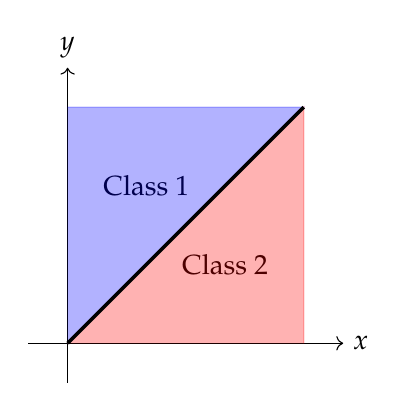
\begin{tikzpicture}
  \draw[->] (-0.5, 0) -- (3.5, 0) node[right] {$x$};
  \draw[->] (0, -0.5) -- (0, 3.5) node[above] {$y$};
  \node at (1, 2) (c1) {Class 1};
  \node at (2, 1) (c2) {Class 2};
  \draw[-, fill, blue, opacity=.3] (0, 3) -- (3, 3) -- (0, 0);
  \draw[-, fill, red, opacity=.3] (3, 0) -- (3, 3) -- (0, 0);
  \draw[scale=1, domain=0:3, smooth, variable=\x, black, line width=0.45mm] plot ({\x}, {\x});
  %\draw[scale=0.5, domain=-3:3, smooth, variable=\y, red]  plot ({\y*\y}, {\y});
\end{tikzpicture}

Furthermore, if the output of $F$ are \emph{probabilities} which add to one, then all points of $x$ will map to the orange line:

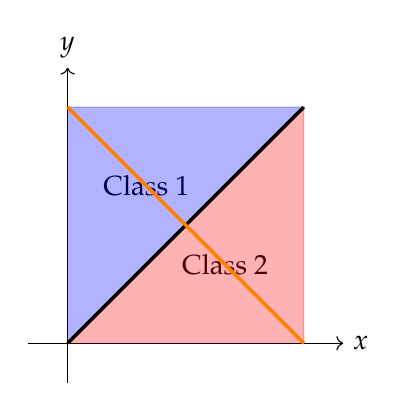
\begin{tikzpicture}
  \draw[->] (-0.5, 0) -- (3.5, 0) node[right] {$x$};
  \draw[->] (0, -0.5) -- (0, 3.5) node[above] {$y$};
  \node at (1, 2) (c1) {Class 1};
  \node at (2, 1) (c2) {Class 2};
  \draw[-, fill, blue, opacity=.3] (0, 3) -- (3, 3) -- (0, 0);
  \draw[-, fill, red, opacity=.3] (3, 0) -- (3, 3) -- (0, 0);
  \draw[scale=1, domain=0:3, smooth, variable=\x, black, line width=0.45mm] plot ({\x}, {\x});
  \draw[-, orange, line width=0.45mm] (0,3) -- (3, 0);
  %\draw[scale=0.5, domain=-3:3, smooth, variable=\y, red]  plot ({\y*\y}, {\y});
\end{tikzpicture}

We note that the point $(0.5, 0.5)$ is therefore the only point on the decision boundary for probability valued $F$. We may generalize to higher dimensions where all probability valued models $F$ will map into the the plane $x + y + z + \cdots = 1$ in $Y$ and the decision boundary will be partitioned into $K-1$ components, where the $K$-decision boundary is the intersection of this plane with the \emph{centroid} line $x = y = z = \cdots$ and the $2$-decision boundaries become planes intersecting at the same line. 

\section{Properties of Decision Boundaries}

In practice, decision boundaries have a variety of properties. The
decision boundary is a pre-image under an onto function that is not
1-1, which allows decision boundaries to vary in upto as many
dimensions as the data space. In practice, this will likely be many
fewer. In particular, decision boundaries should correspond with the
structure of the data. If the data is embedded within a k-manifold
within the input space, the decision boundary can be though of on the
dual space of that manifold.

The dual space of a $k$-manifold embedded in an $n$-dimensional Euclidean space is the space of differential $k$-forms on the manifold. More precisely, for a $k$-manifold $M$ embedded in an $n$-dimensional Euclidean space, the dual space is defined as the space of covariant $k$-tensors on $M$, denoted by $\Lambda^k(M)$, which consists of all linear maps from the tangent space of $M$ at each point to the real numbers.

In particular, when $M$ is a smooth $k$-dimensional manifold, $\Lambda^k(M)$ is the space of smooth $k$-forms on $M$, which can be locally expressed as linear combinations of differential forms of the form $dx_I = dx_{i_1} \wedge dx_{i_2} \wedge \cdots \wedge dx_{i_k}$, where the indices $i_1 < i_2 < \cdots < i_k$ denote the coordinates of a $k$-dimensional chart on $M$ and $dx_i$ denotes the differential of the $i$-th coordinate function.

Intuitively, a $k$-form on $M$ assigns to each $k$-dimensional oriented subspace of the tangent space at a point a signed volume, and the space of all such $k$-forms forms the dual space of $M$. This dual space is important in various areas of mathematics and physics, including differential geometry, topology, and gauge theory.

\subsection{Delaunay Decision Boundaries}

The simplest special case within this dual space is a classifier which
is defined using the Voronoi diagram for the dataset. We can use the
voronoi diagram to define a classifier for an arbitrary query point by
simply assigning it the class of the training point whose voronoi cell
contains it. This has several useful properties, though one in
particular stands out.

Given two points $x$ and $y$ in the training set $X$ which define a delaunay
triangulation and its corresponding voronoi diagram (which is the dual
of the delaunay triangulation) we can see that a line connecting $x$ to
$y$ must orthogonally cross the decision boundary -- which is exactly the voronoi
diagram of this dataset.

Proof:
\begin{proof}
Let $x$ and $y$ be two points in a dataset $X$ that share an edge in the Delaunay triangulation for $X$, and let $e$ be the edge they share in the Delaunay graph. Suppose that $e$ is not orthogonal to the face of the Voronoi diagram that $x$ and $y$ share. Then there exists a point $z$ in the interior of the Voronoi cell for $x$ and $y$ such that the line through $z$ and the midpoint of $e$ intersects the face of the Voronoi diagram at a point $p$.

Since $z$ is in the Voronoi cell for $x$ and $y$, it follows that $d(z, x) < d(z, y)$ (where $d$ is the Euclidean distance). But this contradicts the fact that $x$ and $y$ share an edge in the Delaunay triangulation, which implies that the circumcircle of the triangle formed by $x$, $y$, and $z$ does not contain any other points in $X$. In particular, this means that the circumcenter of this triangle lies on the perpendicular bisector of $e$, which implies that $e$ is orthogonal to the face of the Voronoi diagram that $x$ and $y$ share.

Therefore, we have shown that if $x$ and $y$ share an edge in the Delaunay triangulation for $X$, then the edge they share in the Delaunay graph must be orthogonal to the face of the Voronoi diagram that they share.
\end{proof}
It is immediately clear that for points not in the training set,
the line connecting them with eachother or with a point in the
training set need not cross orthogonal to the voronoi cell
boundaries. In order to talk clearly about such non-orthogonal
crossings, we will define
\begin{definition}
In arbitrary dimensional space, the \emph{angle of incidence} between a line and a plane is defined as the angle between the line and its projection onto the plane, measured in the plane.

More precisely, let $\mathbb{R}^n$ be an $n$-dimensional Euclidean space, let $\ell$ be a line in $\mathbb{R}^n$ with direction vector $\vec{v}$, and let $P$ be a plane in $\mathbb{R}^n$ with normal vector $\vec{n}$. Suppose that $\ell$ intersects $P$ at a point $Q$. Let $H$ be the orthogonal projection of $\ell$ onto $P$, and let $\theta$ be the angle between $\ell$ and $H$.

Then, the angle of incidence between $\ell$ and $P$ is defined as $\alpha = \frac{\pi}{2} - \theta$, where $\pi$ is the constant representing the ratio of the circumference of a circle to its diameter.

Note that when $n=3$, this definition reduces to the familiar definition of the angle of incidence between a line and a plane in three-dimensional space. However, the definition is valid for arbitrary dimensional space.
\end{definition}

and
\begin{definition}
The 
\end{definition}

\subsection{Level Set Definition}
\begin{definition}
The \emph{decision boundary} $D$ of a probability valued function $F$
is a union of all level sets $L_{c_1, c_2, a}$ defined by two classes
$c_1$ and $c_2$ and a constant $a$ which satisfy two properties:
First, given $x \in L_{c_1, c_2, a}$, $F(x)_{c_1} = F(x)_{c_2} = a$
where $a$ is a constant also defining the level set. Second, for all
$c \notin \{c_1, c_2\}$, we have $a > F(x)_c$. This is the
\emph{decision level set} for level $a$. For a given point $x$ on the
decision boundary of a function, the \emph{decision level} is the
value $a$ defining the level set of the decision boundary of which $x$
is a member.

\textbf{Note: } Any point $x$ can be in at most one level set of the
decision boundary. 

\end{definition}

\begin{definition}
  The \emph{dimension} of the decision boundary at a point $x$ is the
  number of dimensions needed to span $\{z : (x + z)$ is in the decision
    level $a$ of the level set containing $x\}$
\end{definition}

A primary property of interest in adversariall attacks is
``sharpness'' i.e. the property that a partition of a set which is
attributed to one class might stab needle-like into a partition of
another set. We will investigate this ``sharpness'' concept by
examining both the incident angle (the acuteness of angles in the
decision boundary) and the dimension of the decision boundary, since
both properties behave like one another. 

There is one conditional bound which is specifically for
voronoi cells which are not exterior to the voronoi diagram. Such
cells are bounded. The line connecting a point within a bounded cell
to the point defining any adjacent voronoi cell.

\subsection{Weighted Delaunay Decision Boundaries}
This simple voronoi classifier has the limitation that it only cares
about which individual training datapoint is closest to the query
point, but is not sensitive to the distribution of this data. If we
suppose that this data is distributed on a manifold with significant
co-dimension with respect to the ambient data space, then it would be
best to use a metric based on this manifold, so that distance among
the data, and hence the delaunay triangulation and the comensurate
voronoi cells would be determined by this metric and thus properly
sensitive to the underlying geometry of this distribution. Alas, this
is akin to having the generating function for nature. It cannot be
computed. So instead, we can take advantage of the Delaunay
triangulation with the usual euclidean metric as an approximation of
the lower dimensional manifold in this case.

This method is limited by the quality of the training dataset as a
sampling of the distribution in question. The Delaunay triangulation
is very sensitive to outliers from a distribution, meaning that our
samples must have relatively little noise in order to be treated as
appropriate samples from the low-dimensional manifold. Second,
Delaunay triangulations are unstable in high-dimensions where very
small triangles are more likely. Both of these problems are lessened
by using data which are sufficiently plentiful relative to the
dimension of the lower dimensional manifold and by requiring that they
do not have more than a small amount of noise to perturb them from the
low dimensional manifold. 

Suppose the lower dimensional manifold $M$ could be defined, and the
training dataset $X$ could be projected onto $M$. The decision
boundary partitioning $M$ would be a set of slices orthogonal to $M$
which would partition any training dataset $X$ into its appropriate
parts. In particular, for a sufficiently dense sampling $x$, we could
define this decision boundary by examining the data points immediately
on either side the decision boundary wherever they meet. We can define
an approximation of the decision boundary as the orthogonal partition
that we expect to be equidistant between adjacent points of different
classes for all samplings of training points. % todo refine this language
In fact, we can define this boundary in the limit using delaunay
triangulation:
\begin{definition}
  Let $M$ be a low dimensional manifold and let $X_{\varepsilon}$ be a
  sampling of points on $M$ for which the maximal edge length along
  its Delaunay triangulation $D_{\varepsilon}$ is
  $\varepsilon$. Given a query point $z$, the $\varepsilon-$Delaunay
  weight for class $i$, $w(z)_i$, is the sum of the barycentric coordinates of $z$
  relative to the vertices with label $i$ of the simplex of $D_{\varepsilon}$ which
  contains $z$. The weight vector $\varepsilon$ boundary level set for
  factor $a$, $B_{\varepsilon,a}$ is the level set $\{z \in M :$ for
  all $i$, we have $w(z)_i \leq a$ and for some $i,j$, $w(z)_i =
  w(z)_j = a\}$. The union of all such level sets over $a$ is the
  \emph{$\varepsilon-$Delaunay-Boundary} $B_{\varepsilon}$. 
  \end{definition}

  Remark, we can extend the decision boundary outside of $M$ by simply
  extending the Delaunay-Boundary using the usual euclidean metric. 

  \begin{theorem}
    Given a low dimensional manifold $M$, 
    \begin{align}
      \lim_{\varepsilon \to 0} B_{\varepsilon}(M) = B(M)
    \end{align}
    $B(M)$ is the decision boundary restricted to $M$. 
  \end{theorem}
  
In this way, a particular training set $X$ defines an approximation of
the general Delaunay Decision Boundary which is well defined outside
of $M$. If the decision boundary is smooth, then for a sufficiently
dense training set $X$ which is sufficiently close to $M$, this
approximation can be bounded by $\varepsilon$ and a lipshitz constant
coming from the mean value theorem on the decision boundary.

It is this approximate form of the decision boundary which we may in
practice evaluate. 

\subsection{Orthant and Wedge}

In order to study decision boundaries, we must talk about properties
related to how decision boundaries interact. We desire a test-object
whose dimensionality and acuteness of angle we can control. To this
end we will use the $k-$dimensional orthant:

\begin{definition}
  Given an integer $k$, the \emph{$k$-orthant} in $n$ dimensions is the set $\{x \in \mathbb{R}^{n}$
  such that for every natural number $i \leq k$, $x_i > 0\}$
  \end{definition}

This concept for an orthant can be extended to be acute in arbitrarily
many angles by tipping toward $x$ to form a wedge.

\begin{definition}
  Given integer $k$ and a set of $k-1$ angles $\Theta$, the \emph{$k-\Theta-$wedge} in $n$ dimensions is the set $\{x \in \mathbb{R}^{n}$
  such that $x_1 > 0$ and for every natural number $1 < i \leq k$,
  $x_i > x_1 \tan(\theta_{i-1})\}$. 
  \end{definition}

These objects allow us to control the dimensionality and acuteness of
a decision boundary to test decision boundary metrics. Another recipe
for analysis is standardizing the paths along which we will cross
decision boundaries. We will use two general paths relative to the
wedge for comparison: centerline and $x-$parallel:

\begin{definition}
  The \emph{centerline} $k-\Theta-$wedge crossing is defined along
  the line $x_1 = t$, for $1 < i \leq k$ $x_i = t
  \tan(\theta_{i-1}/2)$, and for $i > k$ $x_i = 0$.\\

  The \emph{$x-\varepsilon-$parallel} $k-\Theta-$wedge crossing is defined along
  the line $x_1 = t$, for $i > 1$ $x_i = \varepsilon$
\end{definition}

Although we can easily determine whether a point is inside or outside
the wedge simply by checking whether it satisfies the conditions
defining the wedge, we also wish to compute the projection or nearest
point on the wedge for an arbitrary query point. This involves solving
for the closest point to a convex object, which can be accomplished by
projection onto convex sets. 

Computing this projection requires we determine which inequalities
have been violated. Each inequality corresponds with a hyper-plane.
\begin{definition}
  Given a finite set of half-planes $Y_i$ in $\mathbb{R}^n$ and a point $x$,
  let $I$ contain all $i$ such that $x \notin Y_i$. Then since the
  intersection of any number of convex sets is convex, $Y_x = \cap_{i \in
    I} Y_i$ is a convex set. Furthermore, there is exactly one point
  $z$ with $|x - z| \leq |x - y|$ for every $y$ in $Y_x$. This is the
  \emph{projection} of $x$ onto $Y_x$.
\end{definition}

In order to compute this point in practice, we must first determine
all half-planes that do not contain $x$ and then perform orthogonal
projection in sequence along these half-planes using Projection onto
Convex Sets ~/cite{vonneuman-pocs}.

\begin{lemma}
  If all half-planes $Y_i$ with corresponding normal vector $v_i$ have
  boundaries $B(Y_i)$ which are mutually orthogonal, i.e. if $\langle
  v_i, v_j\rangle = 0$ for every combination of $i$ and $j$, then
  the nearest point can be solved by iterative projection 
  \begin{align}
    \vectorproj[v_{i_1}]{(\vectorproj[v_{i_2}]{(\vectorproj[v_{i_3}]{...(x)})})}
  \end{align}
\end{lemma}
(~\cite{vonneuman-pocs})

In the case of the upper wedge, the boundaries are not mutually orthogonal, so
simple orthogonal projection is not sufficient. We must explore this
projection in more detail. Really, what we wish to do is project the
query point $x$ onto the intersection of all of its violated
boundaries. Iteratively, we can orthogonaly project onto the first
hyperplane. We will conduct our projection by subtracting a projection
onto a normal vector for each hyperplane. Given a point $x$, a
hyperplane $p_i$ and its normal vector $v_i$, we define 
\begin{align}
\vectorproj[p_i]{(x)} &= x - x \cdot v_i
\end{align}
The normal vectors for our wedge come in two forms. For the orthant,
all of the normals are of the form $v_i = e_i$. For the angled wedge planes,
they are all of the form $w_i = e_i \cos(\theta_i) - e_1
\sin(\theta_i)$ where $i > 1$. We immediately note that $v_i \cdot v_j
= 0$ for every natural number $i$ and $j$ less than the number of
planes $k$. However,
\begin{align}
  w_i \cdot w_j &= \langle e_i \cos(\theta_i) - e_1 \sin(\theta_i), e_j
                  \cos(\theta_j) - e_1 \sin(\theta_j)\rangle\\
                &= e_ie_j\cos(\theta_i)\cos(\theta_j) -
                  e_1e_j\cos(\theta_j)\sin(\theta_j) - e_1e_i
                  \cos(\theta_i)\sin(\theta_j) +
                  e_1^2\sin(\theta_j)\sin(\theta_i)\\
                &= e_1 \sin(\theta_j)\sin(\theta_i)\\
\end{align}
This means that none of the $w_j$ are orthogonal to each-other and
furthermore 
\begin{align}
  v_1 \cdot w_i &= \langle e_1, -e_1 \sin(\theta_i) + e_i
                  \cos(\theta_i) \rangle \\
                  &= -\sin(\theta_i)
\end{align}
We will leave this latter lack or orthogonality for last, and start by
determining how to sequentially orthogonally project onto the
$w_j$. Critically, we need only project onto the intersection of each
$w_i$ with all previously projected $w_j$. We begin by projecting
from within the plane defined by $w_i$ onto the plane defined by
$w_j$. These vectors are not orthogonal, so we must derive a new
plane and its normal vector $w_{ij}$ which is still orthogonal to $w_i$ but
shares the same intersection with the plane defined by $w_j$ along the
same edge. The conditions that must be satisfied are: 
\begin{align}
  w_{ij} \cdot w_j &= 0 \\
  w_{ij} \perp \cap(w_i, w_j)\\
  w_{ij} \cdot (e_1 + e_i \tan \theta_i + e_j \tan \theta_j) &= 0
\end{align}
This third condition is the requirement that $w_{ij}$ is orthogonal to all
vectors in the intersection of planes $i$ and $j$.

We'll attempt to solve these equations by using a variable $a$ to
account for the discrepency needed to solve these equations. 
\begin{align}
  w_{ij} &= w_j + a = e_j \cos \theta_j - e_1 \sin \theta_j + a\\
  a &= a_1e_1 + a_2e_2 + \cdots a_n e_n \\
  w_{ij} \cdot w_i &= \sin \theta_j\sin\theta_i - a_1 \sin\theta_j +
                     a_i \cos \theta_i = 0\\
  w_{ij} \cdot (e_1 + e_i \tan \theta_i + e_j \tan \theta_j) &= a_1 -
                                                               a_i
                                                               \tan
                                                               \theta_i
                                                               + a_j
                                                               \tan \theta_j
\end{align}
Letting $a_1 \neq 0$ requires that $a = e_1 \sin \theta_j - e_j \cos
\theta_j$ which is a degenerate case, so let $a_1 = 0$. For every
$a_k$ not involved in the intersection of planes, they will have zero
dot product, so we can let them all be 0. Then
\begin{align}
  -a_i \cos \theta_i &= \sin \theta_j \sin \theta_i\\
  a_i &= -\sin \theta_j \tan \theta_i\\
  a_j \tan \theta_j &= \sin \theta_j \tan^2 \theta_i\\
  a_j &= \cos \theta_j \tan^2 \theta_i\\
  w_{ij} &= w_j - e_i \sin \theta_j \tan \theta_i + e_j \cos \theta_j
           \tan^2 \theta_i
\end{align}
Projecting once more onto $w_{k}$ which also shares an intersection
with $w_i$ and $w_j$, we gain one parameter and one degree of
freedom.
\begin{align}
  w_{ijk} &= w_k + a = e_k \cos \theta_k - e_1 \sin \theta_k + a\\
  a &= a_1e_1 + a_2e_2 + \cdots a_n e_n \\
  w_{ijk} \cdot w_i &= \sin \theta_k\sin\theta_i - a_1 \sin\theta_k +
                     a_i \cos \theta_i = 0\\
  w_{ijk} \cdot w_j &= \sin \theta_k\sin\theta_j - a_1 \sin\theta_j +
                     a_j \cos \theta_j = 0\\
  w_{ijk} \cdot (e_1 + e_i \tan \theta_i + e_j \tan \theta_j) &= a_1 +
                                                               a_i
                                                               \tan
                                                               \theta_i
                                                               + a_j
                                                               \tan
                                                                \theta_j
                                                                + a_k
                                                                \tan \theta_k
\end{align}
Now, again letting $a_1 = 0$ to avoid a degenerate case and letting
all other components of $a$ be zero, we have:
\begin{align}
  -a_i \cos \theta_i &= \sin \theta_k \sin \theta_i\\
  a_i &= -\sin \theta_k \tan \theta_i\\
  -a_j \cos \theta_j &= \sin \theta_k \sin \theta_j\\
  a_j &= -\sin \theta_k \tan \theta_j\\
  a_k \tan \theta_k &= \sin \theta_k \tan^2 \theta_i + \sin \theta_k \tan^2 \theta_j\\
  a_k &= \cos \theta_k (\tan^2 \theta_i + \tan^2 \theta_j)\\
  w_{ij} = w_j &- e_i \sin \theta_k \tan \theta_i\\
              &- e_j \sin \theta_k \tan \theta_j\\
              &+ e_k \cos \theta_k (\tan^2 \theta_i + \tan^2 \theta_j)
\end{align}
We see now that we can project an arbitrary sequence of such
intersecting surfaces with each $w_{i...k}$ with $a_i = -\sin \theta_k
\tan \theta_i$ for $i$ less than $k$ and $a_k = \cos \theta_k (\sum_{i
  = 1}^k\tan^2 \theta_i)$. 
Now for our projection algorithm, we first determine if all planes are
satisfied ($x \cdot v_i \geq 0$ and $x \cdot w_i \leq 0$ for every
$i$.) If they are, then we will project onto each plane and pick the
nearest point. If they are not all satisfied, now we'll check each
pair of planes $w_i$ and $v_i$. If both are satisfied, we will skip
them, if both are violated, we will set the coordinate in their native
direction $e_i$ to 0. When only one of the two planes for all compute all planes that are
violated by the position of each query point. For each pair of related
planes $w_i$ and $v_i$, there are three cases. Both satisfied, Both
violated, or either or. In the case that both are violated, i.e. $x
\cdot v_i < 0$, then $x_1 < 0$, which is to say the nearest point
within the wedge in these coordinates will be on the origin. When both
conditions are satisfied, we will ignore this plane except 


%%%%%%%%%%%%%%%%

Now, performing orthogonal projection,
we can orthogonally project in sequence for all half-planes not
containing $x$ except for $v_1$ since $e_1$ is not orthogonal to any
of the wedge planes. Once we have projected onto all other violated
planes, if the projection onto $e_1$ is negative, this will mean that
the nearest point to $x$ is the origin. For $i \neq 1$, all these
projections are of the first form. $x - \sum_{i} x \cdot e_i$. The
first projection of the second form can be done by simple orthogonal
projection, however in order to perform the next projection, we must
project onto the intersection of the two half-planes without leaving
the first plane. We'll need a new plane which is orthogonal to the
first plane, but has the same intersection with the second plane. We
can compute what is missing to make this projection orthogonal. We
have
\begin{align}
  w_i \cdot w_j &= \langle e_i \sin(\theta_i) - e_1 \cos(\theta_i), e_j
                  \sin(\theta_j) - e_1 \cos(\theta_j)\rangle\\
                &= e_ie_j\sin(\theta_i)\sin(\theta_j) -
                  e_1e_j\sin(\theta_j)\cos(\theta_j) - e_1e_i
                  \sin(\theta_i)\cos(\theta_j) +
                  e_1^2\cos(\theta_j)\cos(\theta_i)\\
                &= e_1 \cos(\theta_j)\cos(\theta_i)\\
\end{align}

We can solve for a perturbation in the $e_1$ direction which will make
these two normal vectors orthogonal but due to preserving 




\section{exploring boundary curvature with Random Walks}

To analyze decision boundary curvature, we will project samples of points onto the decision boundary and then use Singular Value Decomposition to analyze the \emph{projected points}. In general, this process will involve first selecting two images $x_1$ and $x_2$ for which $C(x_1) \neq C(x_2)$. A point $x_b$ for which $C(x_b)$ is ambiguous between $C(x_1)$ and $C(x_2)$. The resulting sample $X$ will be projected to the decision boundary by either computing a loss function that is minimized when each of the classes $C(X)$ flip from $C(x_1)$ to $C(x_2)$ or vice versa respectively and performing gradient descent, or by interpolating to the parent point of opposite class (so for $x \in X$, if $C(x) = C(x_1)$, we will interpolate from $x$ to $x_2$). 

Once a projection has been found, we will take the singular value decomposition (SVD) of this sample and examine it for degeneracy. 


Initial comparison of SVDs of decision boundary points yields a single dominant singular value which corresponds with the content of the original image on the boundary. All random noise appears to be mostly orthogonal to this. 

Once this vector is removed, the remaining signal is simply the adversarial attack information. 

To get a set of singular vectors which to not emphasize the image content, we take random differences among the sampled images and take the SVD of those random differences. 

In these first 10 images, this procedure is carried out on the orthant, where samples are generated with mean 0 and are projected onto orthants with increasing numbers of dimensions. We can see a very clear dropped set of singular values smaller than the rest, which indicate the number of degenerate dimensions. In each of these cases, the dropped singular values match the dimension of the orthant. 

Experiment : A valid experiment here is to measure the difference between the images and the projection to get -- in this case -- normal vectors to the orthant for each image sampled. The SVD of these normals can be computed to determine the number of dimensions in the projecetion operation. This same procedure can be caried out later in the real practical image projections, although in that case orthogonality is not guaranteed. 

\includegraphics[width=8cm]{img/e03-SVD-Orthant_origin-dim-cropped1.png}
\includegraphics[width=9cm]{img/e03-SVD-Orthant_origin-dim-cropped2.png}
\includegraphics[width=9cm]{img/e03-SVD-Orthant_origin-dim-cropped3.png}
\includegraphics[width=9cm]{img/e03-SVD-Orthant_origin-dim-cropped4.png}
\includegraphics[width=9cm]{img/e03-SVD-Orthant_origin-dim-cropped5.png}
\includegraphics[width=9cm]{img/e03-SVD-Orthant_origin-dim-cropped6.png}
\includegraphics[width=9cm]{img/e03-SVD-Orthant_origin-dim-cropped7.png}
\includegraphics[width=9cm]{img/e03-SVD-Orthant_origin-dim-cropped8.png}
\includegraphics[width=9cm]{img/e03-SVD-Orthant_origin-dim-cropped9.png}
\includegraphics[width=9cm]{img/e03-SVD-Orthant_origin-dim-cropped10.png}

There is a question of how best to measure "normal" vectors for each projection. The most direct computation is to take a sample with small variance around each point on the decision boundary and solve least squares of each of these samples. We have previously observed that \emph{most} of the decision boundary is locally planar. 

It remains to compare these computed normals with other known quantities, e.g. the gradient computed with respect to adversarial loss functions and the difference between each sampled image and its resultant projection. In addition, it remains to compare the normals of multiple nearby images to determine at what radius of sample the decision boundary begins to show curvature.\\

The following image shows singular values in order for a sample around a decision boundary image in MNIST generated by interpolating from a test image to an adversarial image generated from it. This plot is dominated by the natural distribution of singular values for a gaussian and also by the original image information which can be seen as a huge singular value on the far left. We will address both of these factors in following plots. \\

\includegraphics[width=14cm]{img/SVD-rand_diff-decision_boundary_uvar-1.0-index-0-image-999.png}

The following plots are generated with a new distribution to replace the gaussian. This "Flat SVD" distribution is generated by first taking a gaussian sample representable by a matrix $X$, then taking the SVD of this gaussian sample $U \Sigma V = X$, replacing $\Sigma$ by $|\Sigma|_2 I$. This distribution has the property that its SVD is flat, while maintaining the Frobenius norm of $X$. This helps to highlight degeneracy in singular values. \\

These first two plots are generated by sampling around a decision boundary image found by interpolating between two test images (rather than a test image and an adversarial example generated from it). We note that the SVD contains two degernate values. These seem to correpond with the two original images of the interpolation. 

\includegraphics[width=14cm]{img/e05-SVD-uniform-rand_diff-decision_boundary_uvar-0.001-index-0-image-999.png}

\includegraphics[width=14cm]{img/e05-SVD-uniform-rand_diff-decision_boundary_uvar-0.001-index-0-image-999-cropped.png}


These last two images are generated with the flattened distribution 

\includegraphics[width=14cm]{img/e06-SVD-uniform-rand_diff-decision_boundary_uvar-0.0001-index-0-image-999-cropped.png}

\includegraphics[width=14cm]{img/e06-SVD-uniform-rand_diff-decision_boundary_uvar-0.0001-index-0-image-999.png}

What these experiments tell us is that most of the time when we cross a decision oundary in the MNIST Dataset, we are crossing at a plane, however if we examine a slightly larger ball around a given point, it will intersect the decision boundary at many other places. 

\section{Re-Examining Persistence}

A movivating picture in this research is an image generated while interpolating persistence in the beginning of this research. 

\includegraphics[width=15cm]{img/persistence_interpolation-IMNET-class-11-vgg16-BIM-48-attack_data-001 (2).png}

The next objective is to examine this particular case with our random walk and projection Tools. 

We also wish to augment these tools to include 

%%%%%%%%%%%%%%%%%

\subsection{in probability space}
\subsection{in image space}
\section{define orthants}
\section{skewness}

\section{sampling decision boundaries and analyzing dimensionality
with PCA}

\section{neural network attack gradients versus decision boundaries}

\section{skewed orthant recreates persistence picture (?). }
\section{measuring skewness of ANNs}
\section{Relate skewness with dimpled manifold and features not bugs papers}


turn observations into are they a definition, a theorem, or a discussion

decision\_boundary crossing

\bibliographystyle{abbrvnat}
%\bibliography{'../../0-research/bibfile'}
\bibliography{bibfile}


\end{document}
